\chapter[Appendix: Candidate Braids for Track 8]{Appendix: Candidate Braids for Track 8}
\label{app:candidate_braids_track_8}

\section{Summary of Candidate Braid Families}
\label{sec:summary_track8_braids}

Through the exhaustive train track case analysis of Track 8 in the stratum $(2;1^6;3^2)$ (the full details of which are presented in Appendix \ref{app:case_analysis_track8}), we isolate exactly 9 candidate families of train track maps. If the pseudo-Anosov representative $\phi_\Phi$ has no interior fixed points, then its mapping class $\Phi$ must be conjugate to the lift of one of the following 9 braid families (enumerated below with their twist parameters).

\vspace{0.3cm}
\begingroup
\raggedbottom
\begin{enumerate}
    \item $\displaystyle \Delta^{2i} \big( \allowbreak\sigma_{5}^{-1}\allowbreak\sigma_{2}\allowbreak\sigma_{4}^{-1}\allowbreak\sigma_{1}^{-1}\allowbreak\sigma_{2}^{-1}\allowbreak\sigma_{3}^{-1}\allowbreak\sigma_{4}^{-1}\allowbreak\sigma_{5}^{-1}\allowbreak\sigma_{3}^{-1}\allowbreak\sigma_{4}^{-1}\allowbreak\sigma_{2}\allowbreak\sigma_{1}\allowbreak\sigma_{2}\allowbreak\sigma_{3}^{-1}\allowbreak\sigma_{4}^{-1}\allowbreak\sigma_{2}^{-1}\allowbreak\sigma_{1}^{-1} \big)^{-1}$
    \item $\displaystyle \Delta^{2i} \big( \allowbreak\sigma_{5}^{-1}\allowbreak\sigma_{2}\allowbreak\sigma_{4}^{-1}\allowbreak\sigma_{1}^{-1}\allowbreak\sigma_{2}^{-1}\allowbreak\sigma_{3}^{-1}\allowbreak\sigma_{4}^{-1}\allowbreak\sigma_{2}\allowbreak\sigma_{1}\allowbreak\sigma_{2}\allowbreak\sigma_{3}^{-1}\allowbreak\sigma_{5}^{-1}\allowbreak\sigma_{3}^{-1}\allowbreak\sigma_{4}^{-1}\allowbreak\sigma_{3}^{-1}\allowbreak\sigma_{2}^{-1}\allowbreak\sigma_{1}^{-1} \big)^{-1}$
    \item $\displaystyle \Delta^{2i} \big( \allowbreak\sigma_{5}^{-1}\allowbreak\sigma_{2}\allowbreak\sigma_{4}^{-1}\allowbreak\sigma_{1}^{-1}\allowbreak\sigma_{2}^{-1}\allowbreak\sigma_{3}^{-1}\allowbreak\sigma_{4}^{-1}\allowbreak\sigma_{5}^{-1}\allowbreak\sigma_{2}\allowbreak\sigma_{1}\allowbreak\sigma_{3}^{-1}\allowbreak\sigma_{4}^{-1}\allowbreak\sigma_{2}\allowbreak\sigma_{3}^{-1}\allowbreak\sigma_{4}^{-1}\allowbreak\sigma_{2}^{-1}\allowbreak\sigma_{1}^{-1} \big)^{-1}$
    \item $\displaystyle \Delta^{2i} \big( \allowbreak\sigma_{5}^{-1}\allowbreak\sigma_{2}^{-1}\allowbreak\sigma_{1}^{-1}\allowbreak\sigma_{1}^{-1}\allowbreak\sigma_{2}^{-1}\allowbreak\sigma_{3}^{-1}\allowbreak\sigma_{4}^{-1}\allowbreak\sigma_{3}^{-1}\allowbreak\sigma_{3}^{-1}\allowbreak\sigma_{3}^{-1}\allowbreak\sigma_{5}^{-1}\allowbreak\sigma_{4}^{-1}\allowbreak\sigma_{3}^{-1}\allowbreak\sigma_{1}^{-1}\allowbreak\sigma_{2}^{-1}\allowbreak\sigma_{1}^{-1}\allowbreak\sigma_{1}^{-1} \big)^{-1}$
    \item $\displaystyle \Delta^{2i} \big( \allowbreak\sigma_{5}^{-1}\allowbreak\sigma_{4}^{-1}\allowbreak\sigma_{1}^{-1}\allowbreak\sigma_{2}^{-1}\allowbreak\sigma_{1}^{-1}\allowbreak\sigma_{1}^{-1}\allowbreak\sigma_{1}^{-1}\allowbreak\sigma_{2}^{-1}\allowbreak\sigma_{3}^{-1}\allowbreak\sigma_{4}^{-1}\allowbreak\sigma_{3}^{-1}\allowbreak\sigma_{3}^{-1}\allowbreak\sigma_{5}^{-1}\allowbreak\sigma_{4}^{-1}\allowbreak\sigma_{3}^{-1}\allowbreak\sigma_{2}^{-1}\allowbreak\sigma_{1}^{-1} \big)^{-1}$
    \item $\displaystyle \Delta^{2i} \big( \allowbreak\sigma_{5}^{-1}\allowbreak\sigma_{1}^{-1}\allowbreak\sigma_{2}^{-1}\allowbreak\sigma_{4}^{-1}\allowbreak\sigma_{3}^{-1}\allowbreak\sigma_{4}^{-1}\allowbreak\sigma_{5}^{-1}\allowbreak\sigma_{3}^{-1}\allowbreak\sigma_{3}^{-1}\allowbreak\sigma_{4}^{-1}\allowbreak\sigma_{3}^{-1}\allowbreak\sigma_{2}^{-1}\allowbreak\sigma_{1}^{-1}\allowbreak\sigma_{1}^{-1}\allowbreak\sigma_{2}^{-1}\allowbreak\sigma_{1}^{-1}\allowbreak\sigma_{1}^{-1} \big)^{-1}$
    \item $\displaystyle \Delta^{2i} \big( \allowbreak\sigma_{5}^{-1}\allowbreak\sigma_{4}^k\allowbreak\sigma_{3}\allowbreak\sigma_{1}^{-1}\allowbreak\sigma_{2}^{-1}\allowbreak\sigma_{3}^{-1}\allowbreak\sigma_{4}^{-1}\allowbreak\sigma_{3}\allowbreak\sigma_{3}\allowbreak\sigma_{2}\allowbreak\sigma_{1}\allowbreak\sigma_{4}\allowbreak\sigma_{3}\allowbreak\sigma_{2}\allowbreak\sigma_{4}\allowbreak\sigma_{3} \cdot \Lambda_6 \cdot J \big)^{-1}$
    \item $\displaystyle \Delta^{2i} \big( \allowbreak\sigma_{5}^{-1}\allowbreak\sigma_{1}^{-1}\allowbreak\sigma_{2}^{-1}\allowbreak\sigma_{3}^{-1}\allowbreak\sigma_{4}^{-1}\allowbreak\sigma_{3}\allowbreak\sigma_{2}\allowbreak\sigma_{1}\allowbreak\sigma_{2}^{-1}\allowbreak\sigma_{3}^{-1}\allowbreak\sigma_{2}\allowbreak\sigma_{3}\allowbreak\sigma_{3}\allowbreak\sigma_{2}\allowbreak\sigma_{1}\allowbreak\sigma_{4}\allowbreak\sigma_{3}\allowbreak\sigma_{2}\allowbreak\sigma_{4}\allowbreak\sigma_{3} \cdot \Lambda_6 \cdot J \big)^{-1}$
    \item $\displaystyle \Delta^{2i} \big( \allowbreak\sigma_{1}^{-1}\allowbreak\sigma_{2}^{-k}\allowbreak\sigma_{3}^{-1}\allowbreak\sigma_{2}^{-1}\allowbreak\sigma_{2}^{-1}\allowbreak\sigma_{3}^{-1}\allowbreak\sigma_{2}^{-1}\allowbreak\sigma_{2}^{-1}\allowbreak\sigma_{1}\allowbreak\sigma_{2}\allowbreak\sigma_{3}\allowbreak\sigma_{4}\allowbreak\sigma_{5} \cdot \Lambda_6 \cdot J \big)^{-1}$
\end{enumerate}
\endgroup

\clearpage

\section{Base Braids \texorpdfstring{$\Lambda_6$}{Lambda\_6} and \texorpdfstring{$J$}{J}}
Before we list the braids carrying candidate train track maps for Track 8, we introduce the following base braids, which we will call $\Lambda_6$ and $J$:

\begin{flushleft}
$\displaystyle \Lambda_6 = \allowbreak\sigma_{1}\allowbreak\sigma_{2}\allowbreak\sigma_{1}\allowbreak\sigma_{3}\allowbreak\sigma_{2}\allowbreak\sigma_{1}\allowbreak\sigma_{4}\allowbreak\sigma_{3}\allowbreak\sigma_{2}\allowbreak\sigma_{1}\allowbreak\sigma_{5}\allowbreak\sigma_{4}\allowbreak\sigma_{3}\allowbreak\sigma_{2}\allowbreak\sigma_{1}$
\end{flushleft}

\begin{flushleft}
$\displaystyle J = \allowbreak\sigma_{1}^{-1}\allowbreak\sigma_{2}^{-1}\allowbreak\sigma_{1}^{-1}\allowbreak\sigma_{5}\allowbreak\sigma_{4}\allowbreak\sigma_{5}$
\end{flushleft}

We shall make use of $\Lambda_6$ and $J$ occasionally in constructing candidate braids for Track 8.

\clearpage

\section{Candidate Family 1 (Anomy)}\label{sec:track8_anomy}
Train Track Map Candidate Family 1 of Track 8 is shown in Figure \ref{fig:track8_braid_b8_1_map}. See \ref{Anomy} for details.

\begin{figure*}[ht]
    \centering
    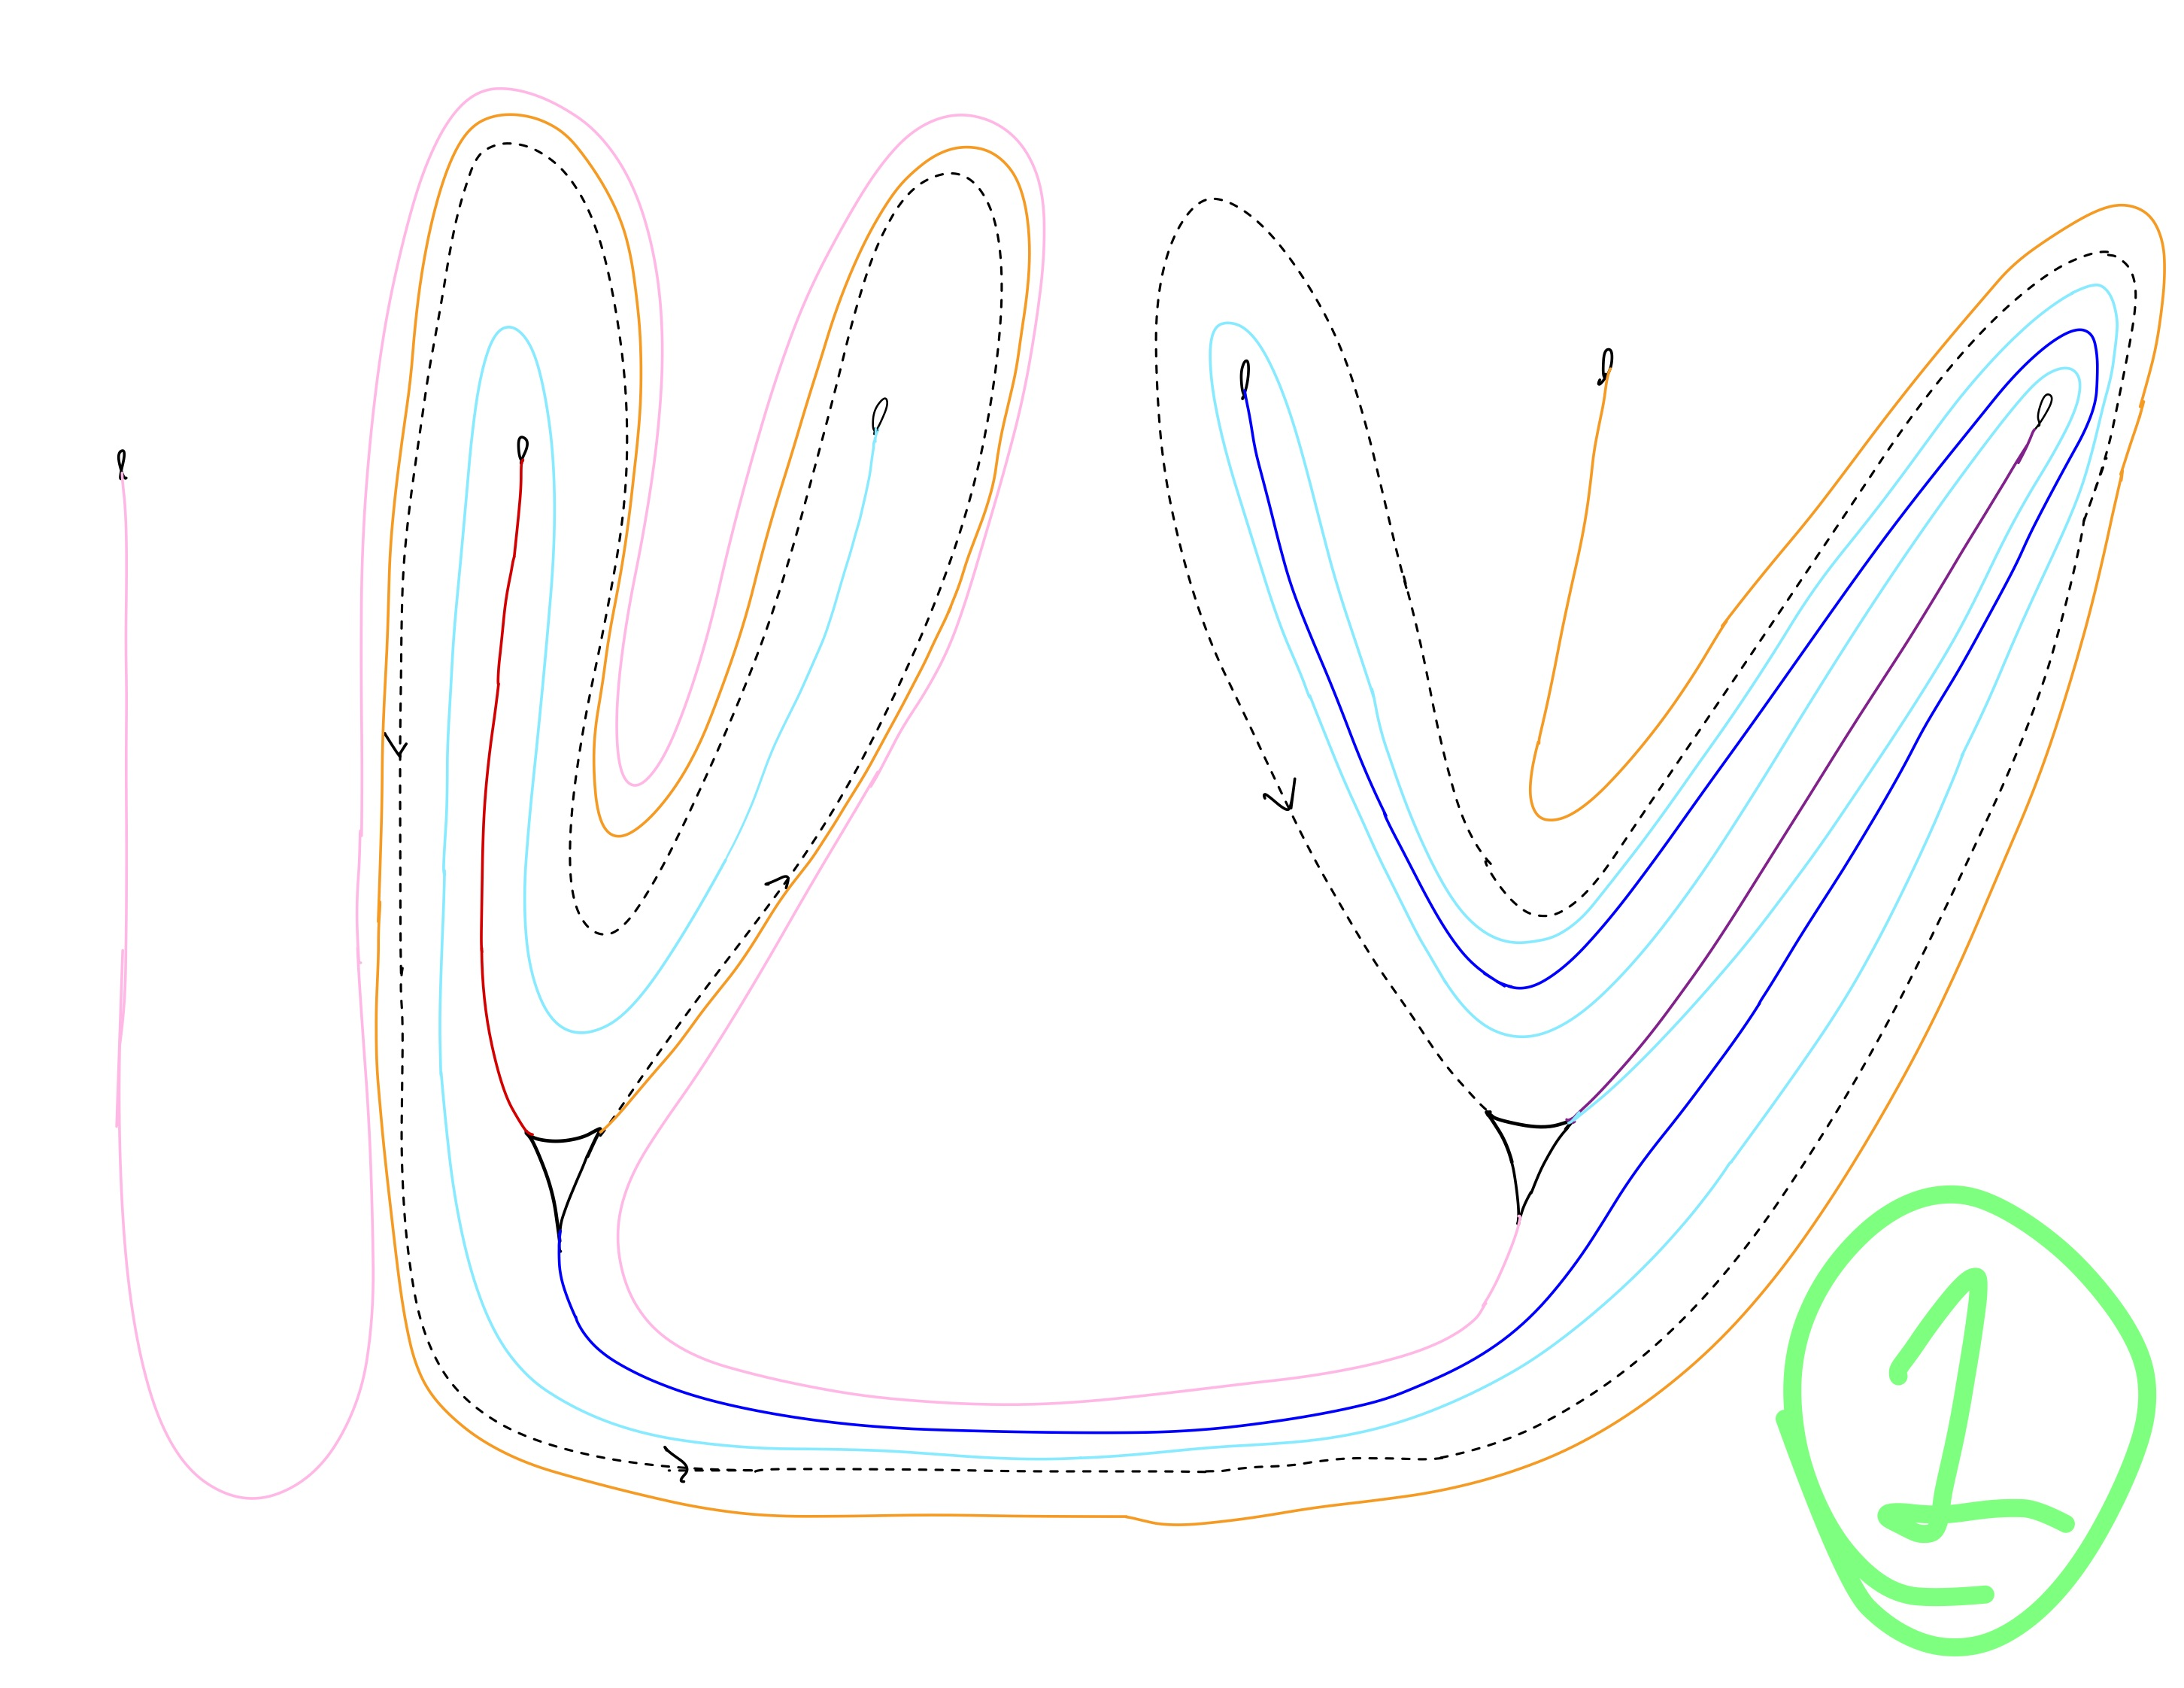
\includegraphics[width=\linewidth, height=0.45\textheight, keepaspectratio]{figures_braid/figures_track_8/Track 8 Braid 1 Anomy-1.jpg}
    \caption{Train Track Map Candidate Family 1 (Anomy) of Track 8.}
    \label{fig:track8_braid_b8_1_map}
\end{figure*}

The inverse of the following braid carries this family of train track maps:
\[
b_1^8 = \sigma_{5}^{-1} \sigma_{2} \sigma_{4}^{-1} \sigma_{1}^{-1} \sigma_{2}^{-1} \sigma_{3}^{-1} \sigma_{4}^{-1} \sigma_{5}^{-1} \sigma_{3}^{-1} \sigma_{4}^{-1} \sigma_{2} \sigma_{1} \sigma_{2} \sigma_{3}^{-1} \sigma_{4}^{-1} \sigma_{2}^{-1} \sigma_{1}^{-1}
\]

This is shown in Figure \ref{fig:track8_braid_b8_1}.

\begin{figure*}[p]
    \centering
    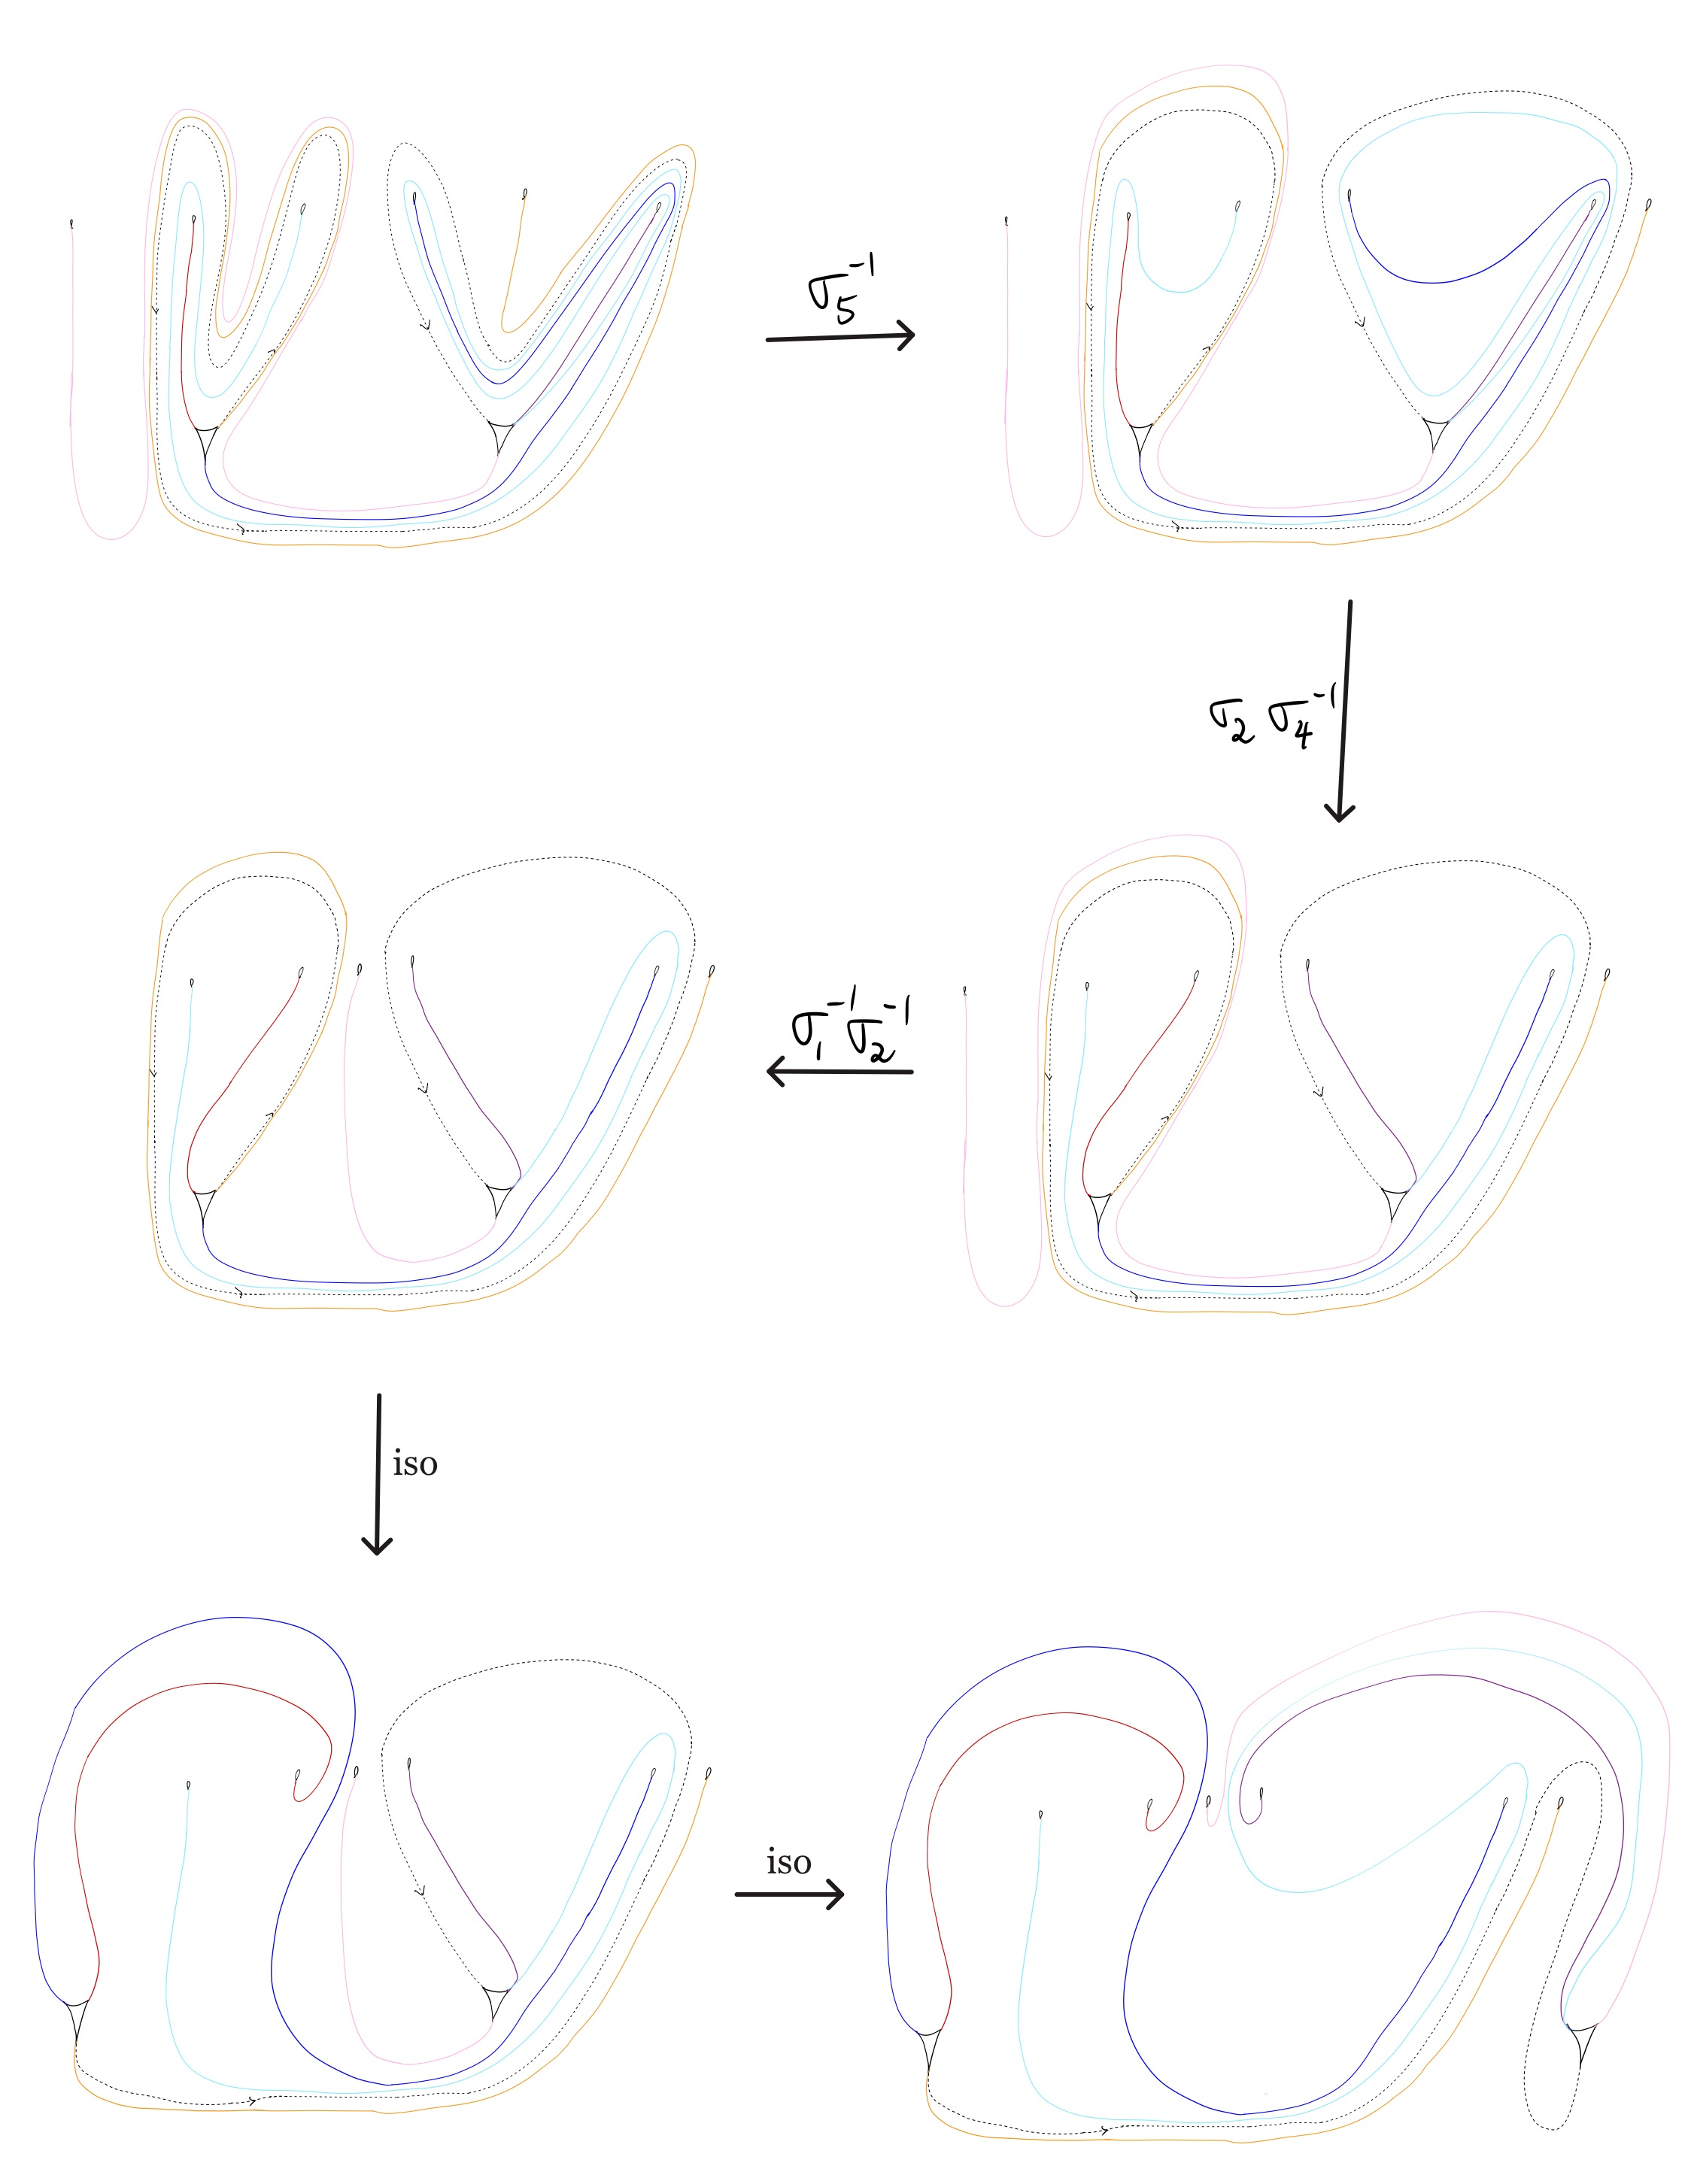
\includegraphics[width=\linewidth, height=0.45\textheight, keepaspectratio]{figures_braid/figures_track_8/Track 8 Braid 1 Anomy-2.jpg}%
    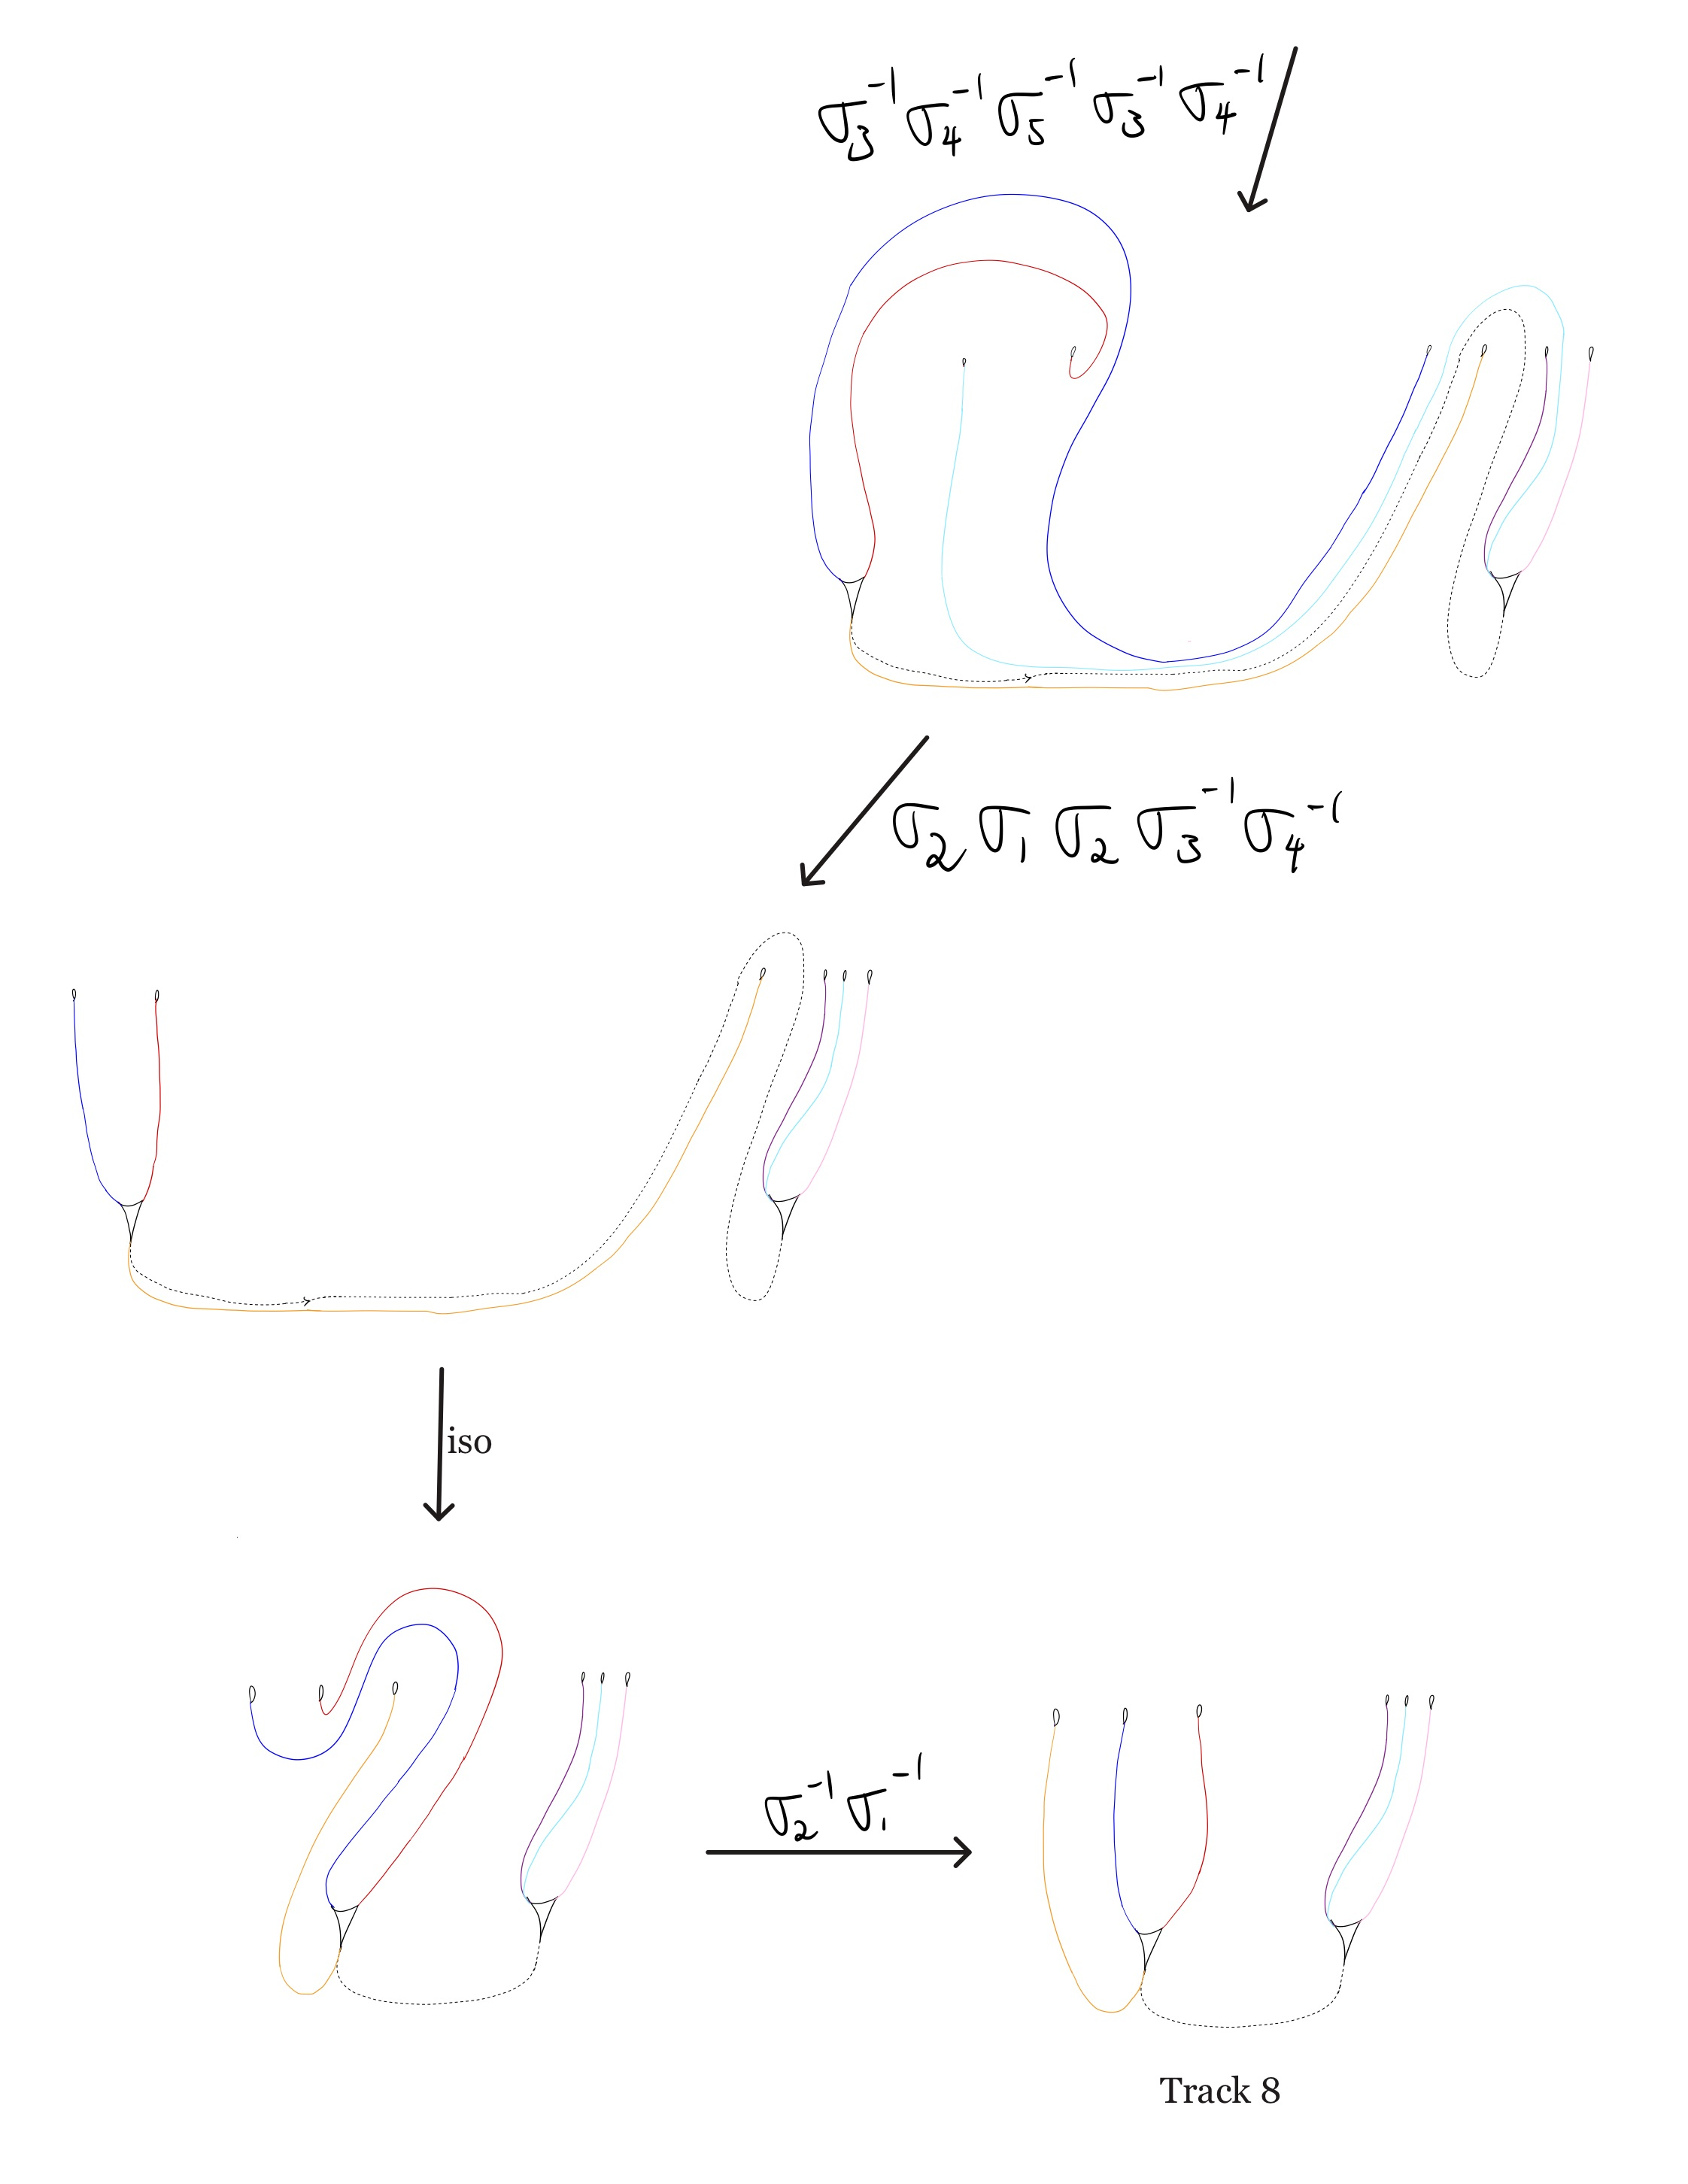
\includegraphics[width=\linewidth, height=0.45\textheight, keepaspectratio]{figures_braid/figures_track_8/Track 8 Braid 1 Anomy-3.jpg}
    \caption{This sequence shows the inverse of the braid $b_1^8$ carries Train Track Candidate Family 1.}
    \label{fig:track8_braid_b8_1}
\end{figure*}

\clearpage

\section{Candidate Family 2 (Diatree)}\label{sec:track8_diatree}
Train Track Map Candidate Family 2 of Track 8 is shown in Figure \ref{fig:track8_braid_b8_2_map}. See \ref{Diatree} for details.

\begin{figure*}[ht]
    \centering
    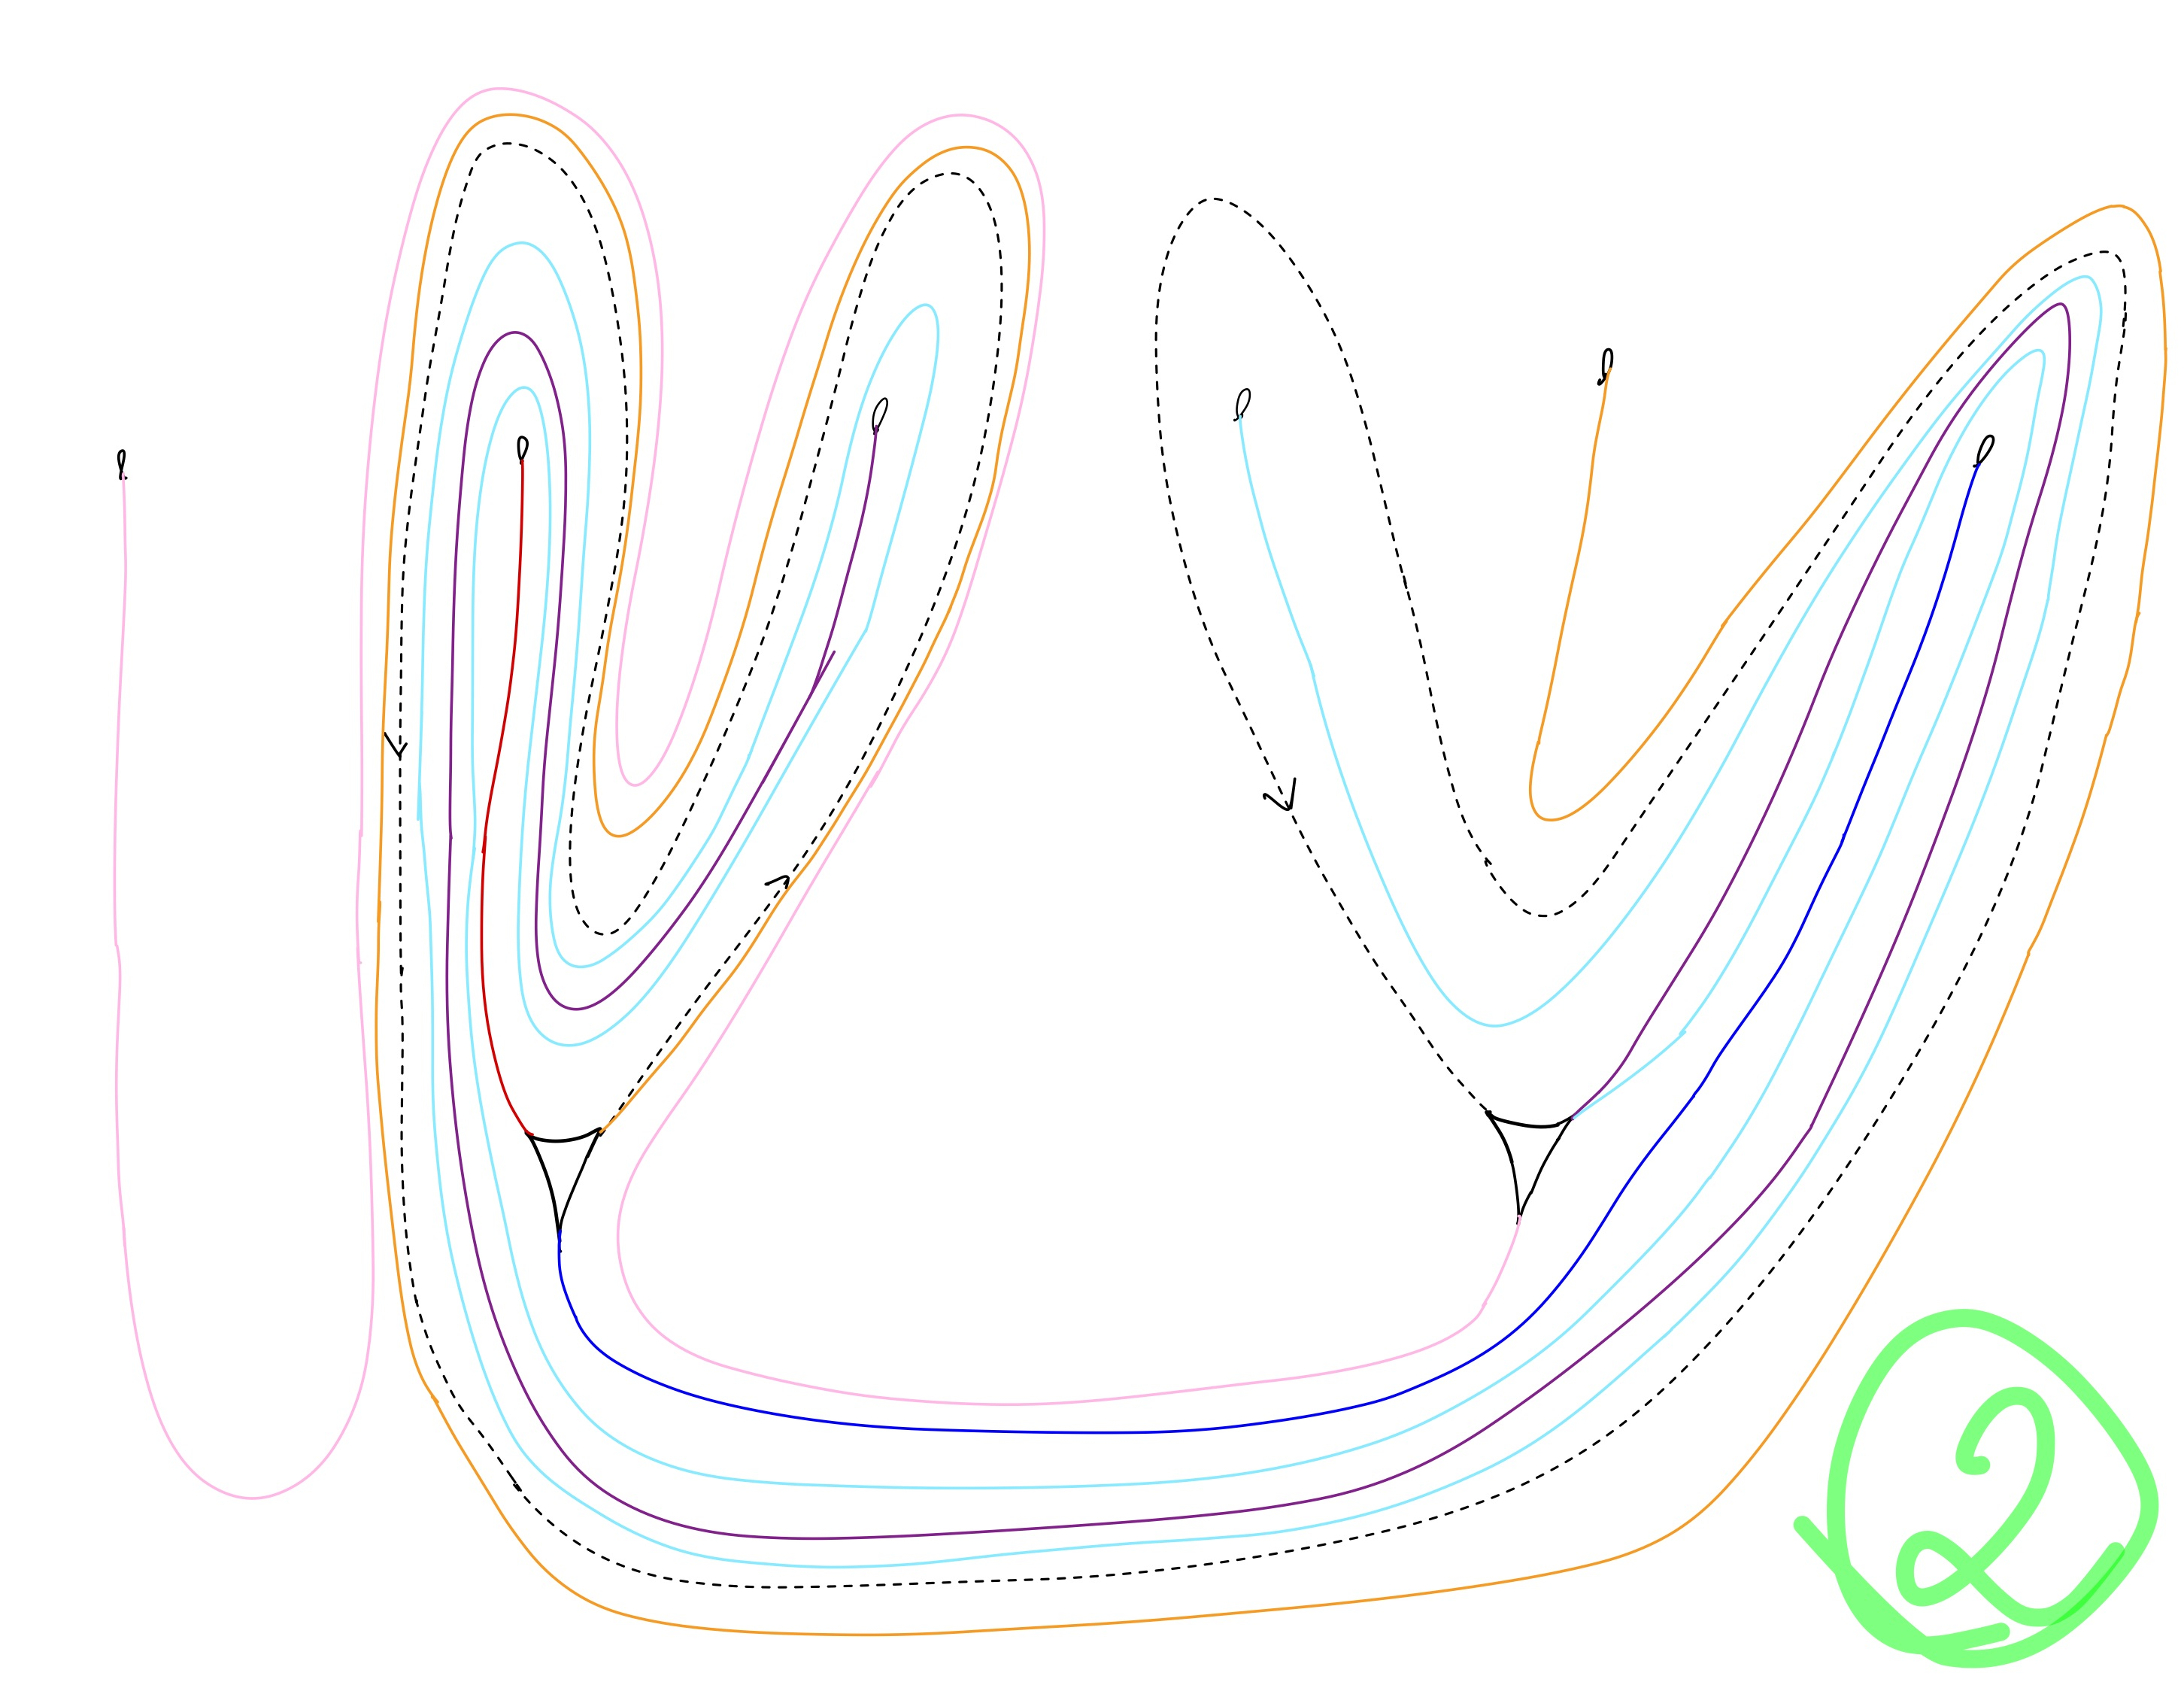
\includegraphics[width=\linewidth, height=0.45\textheight, keepaspectratio]{figures_braid/figures_track_8/Track 8 Braid 2 Diatree-1.jpg}
    \caption{Train Track Map Candidate Family 2 (Diatree) of Track 8.}
    \label{fig:track8_braid_b8_2_map}
\end{figure*}

The inverse of the following braid carries this family of train track maps:
\[
b_2^8 = \sigma_{5}^{-1} \sigma_{2} \sigma_{4}^{-1} \sigma_{1}^{-1} \sigma_{2}^{-1} \sigma_{3}^{-1} \sigma_{4}^{-1} \sigma_{2} \sigma_{1} \sigma_{2} \sigma_{3}^{-1} \sigma_{5}^{-1} \sigma_{3}^{-1} \sigma_{4}^{-1} \sigma_{3}^{-1} \sigma_{2}^{-1} \sigma_{1}^{-1}
\]

This is shown in Figure \ref{fig:track8_braid_b8_2}.

\begin{figure*}[p]
    \centering
    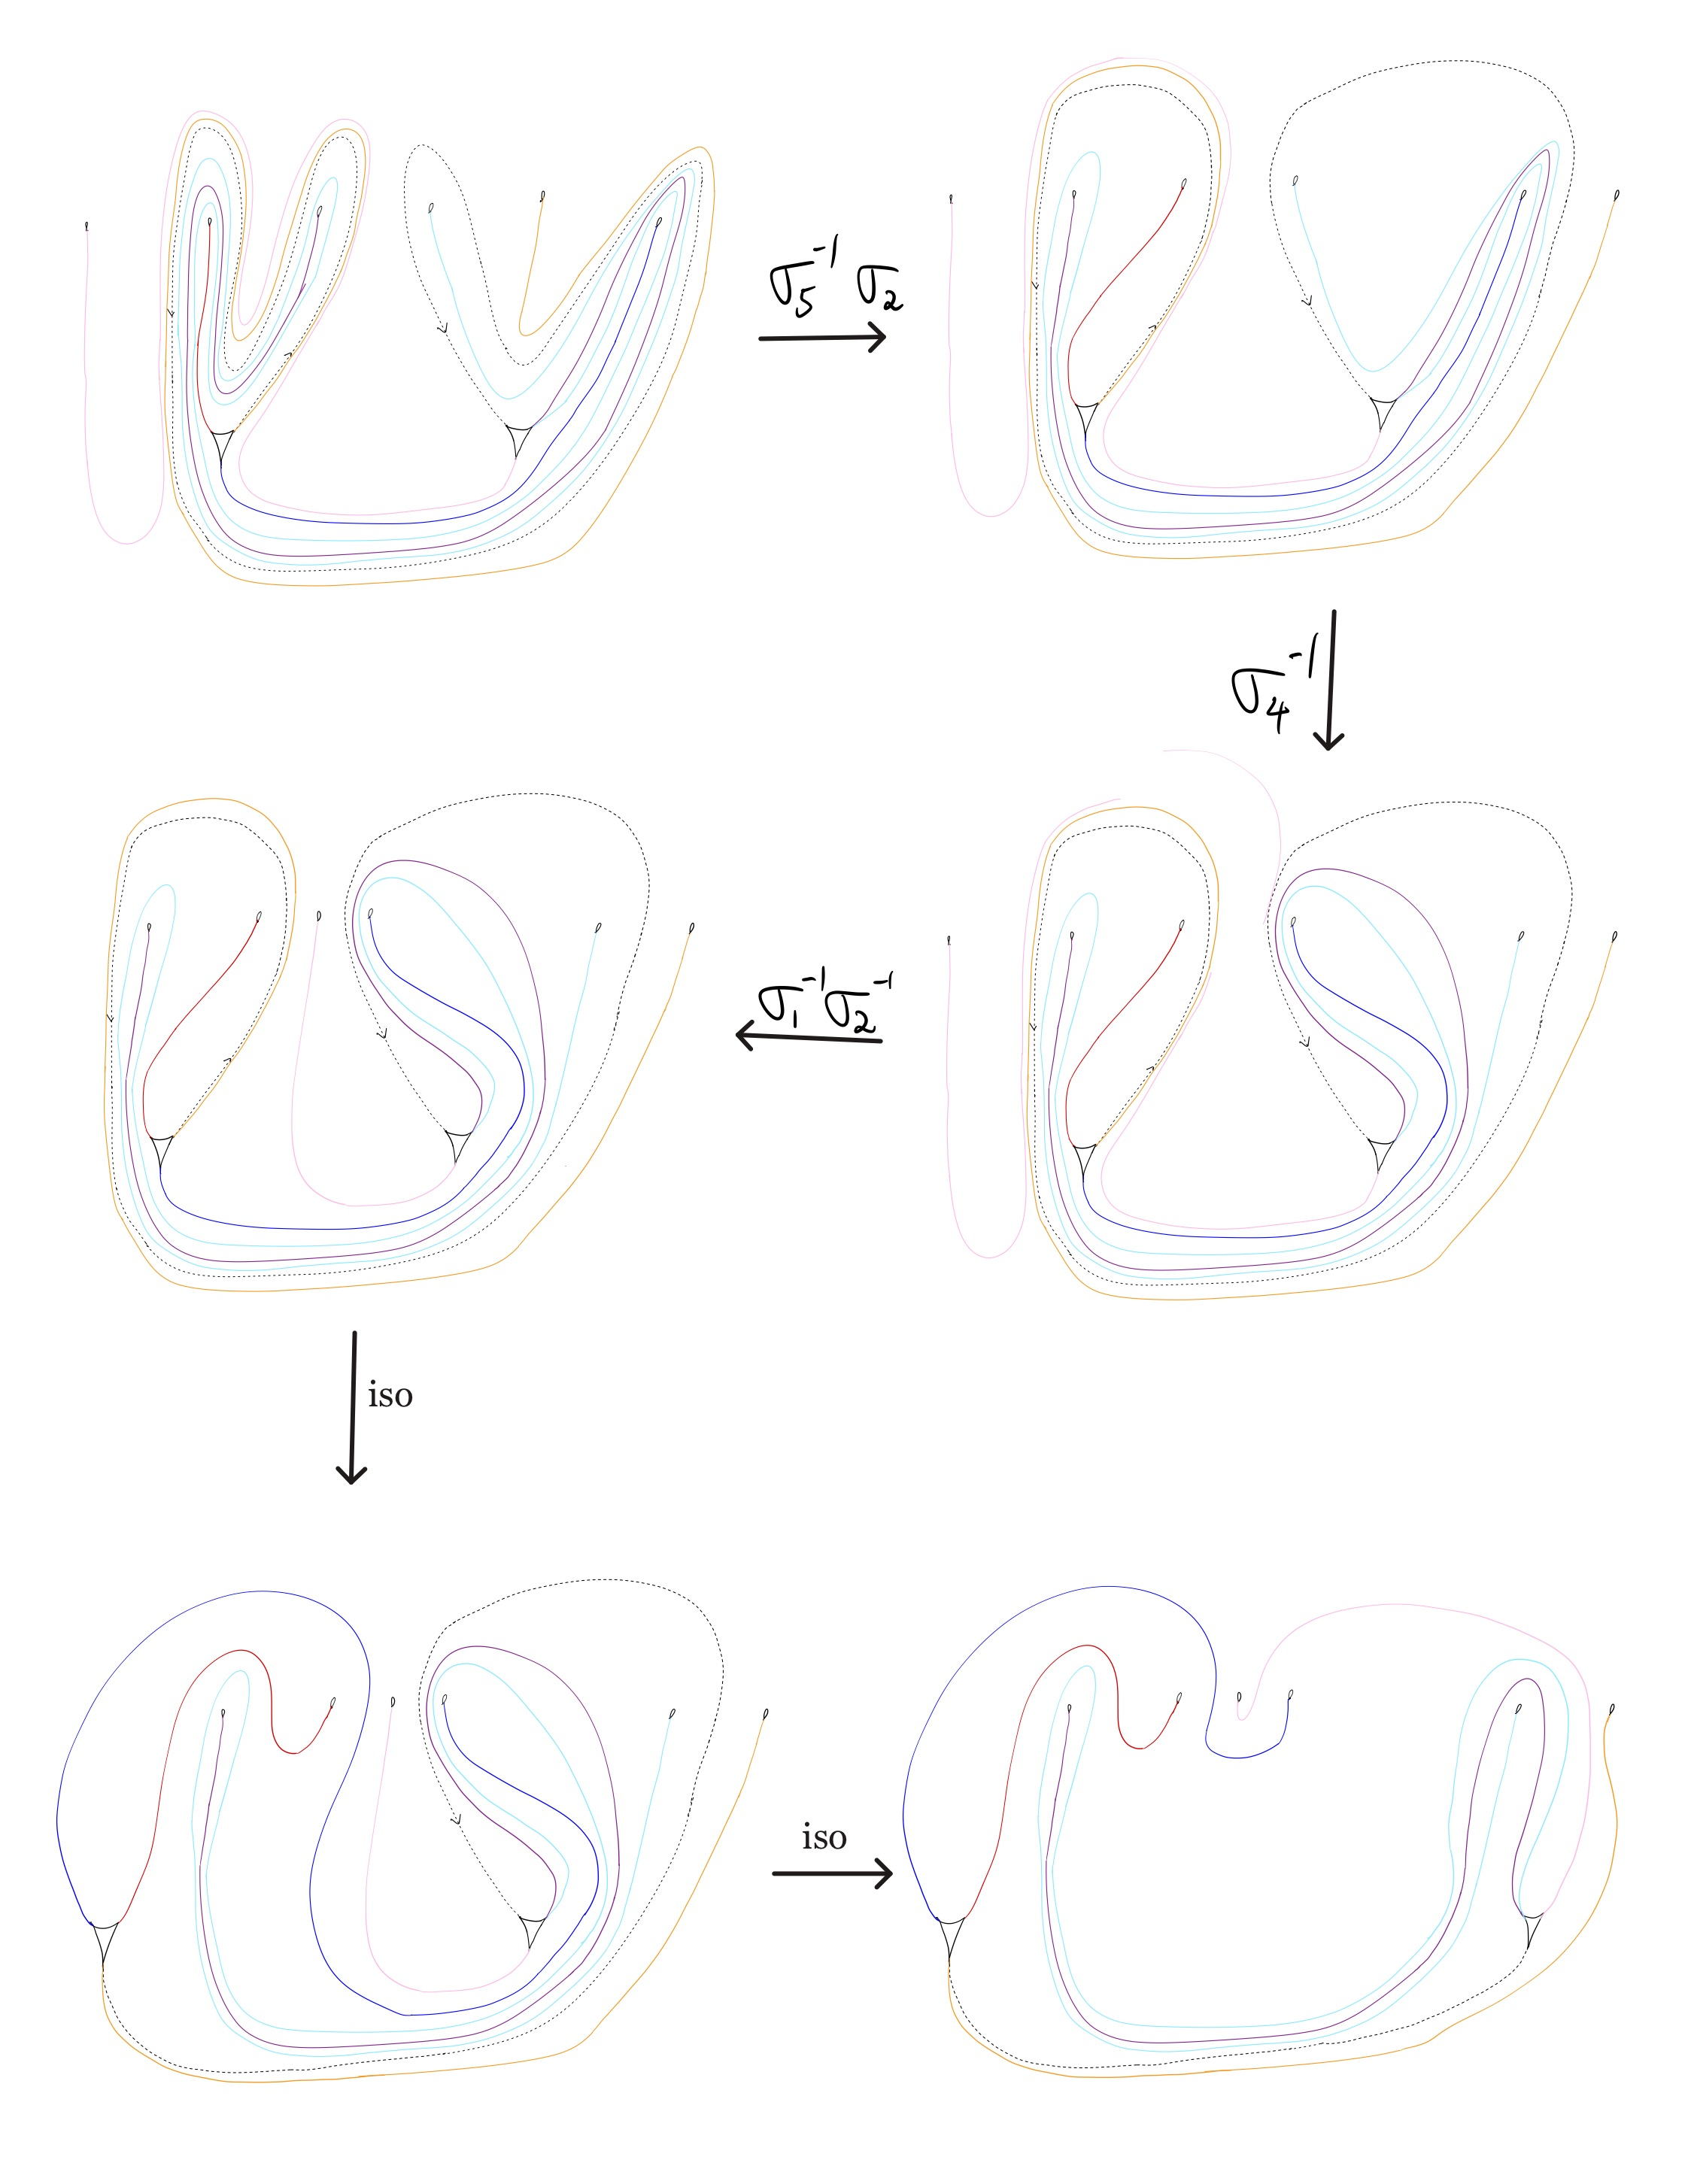
\includegraphics[width=\linewidth, height=0.45\textheight, keepaspectratio]{figures_braid/figures_track_8/Track 8 Braid 2 Diatree-2.jpg}%
    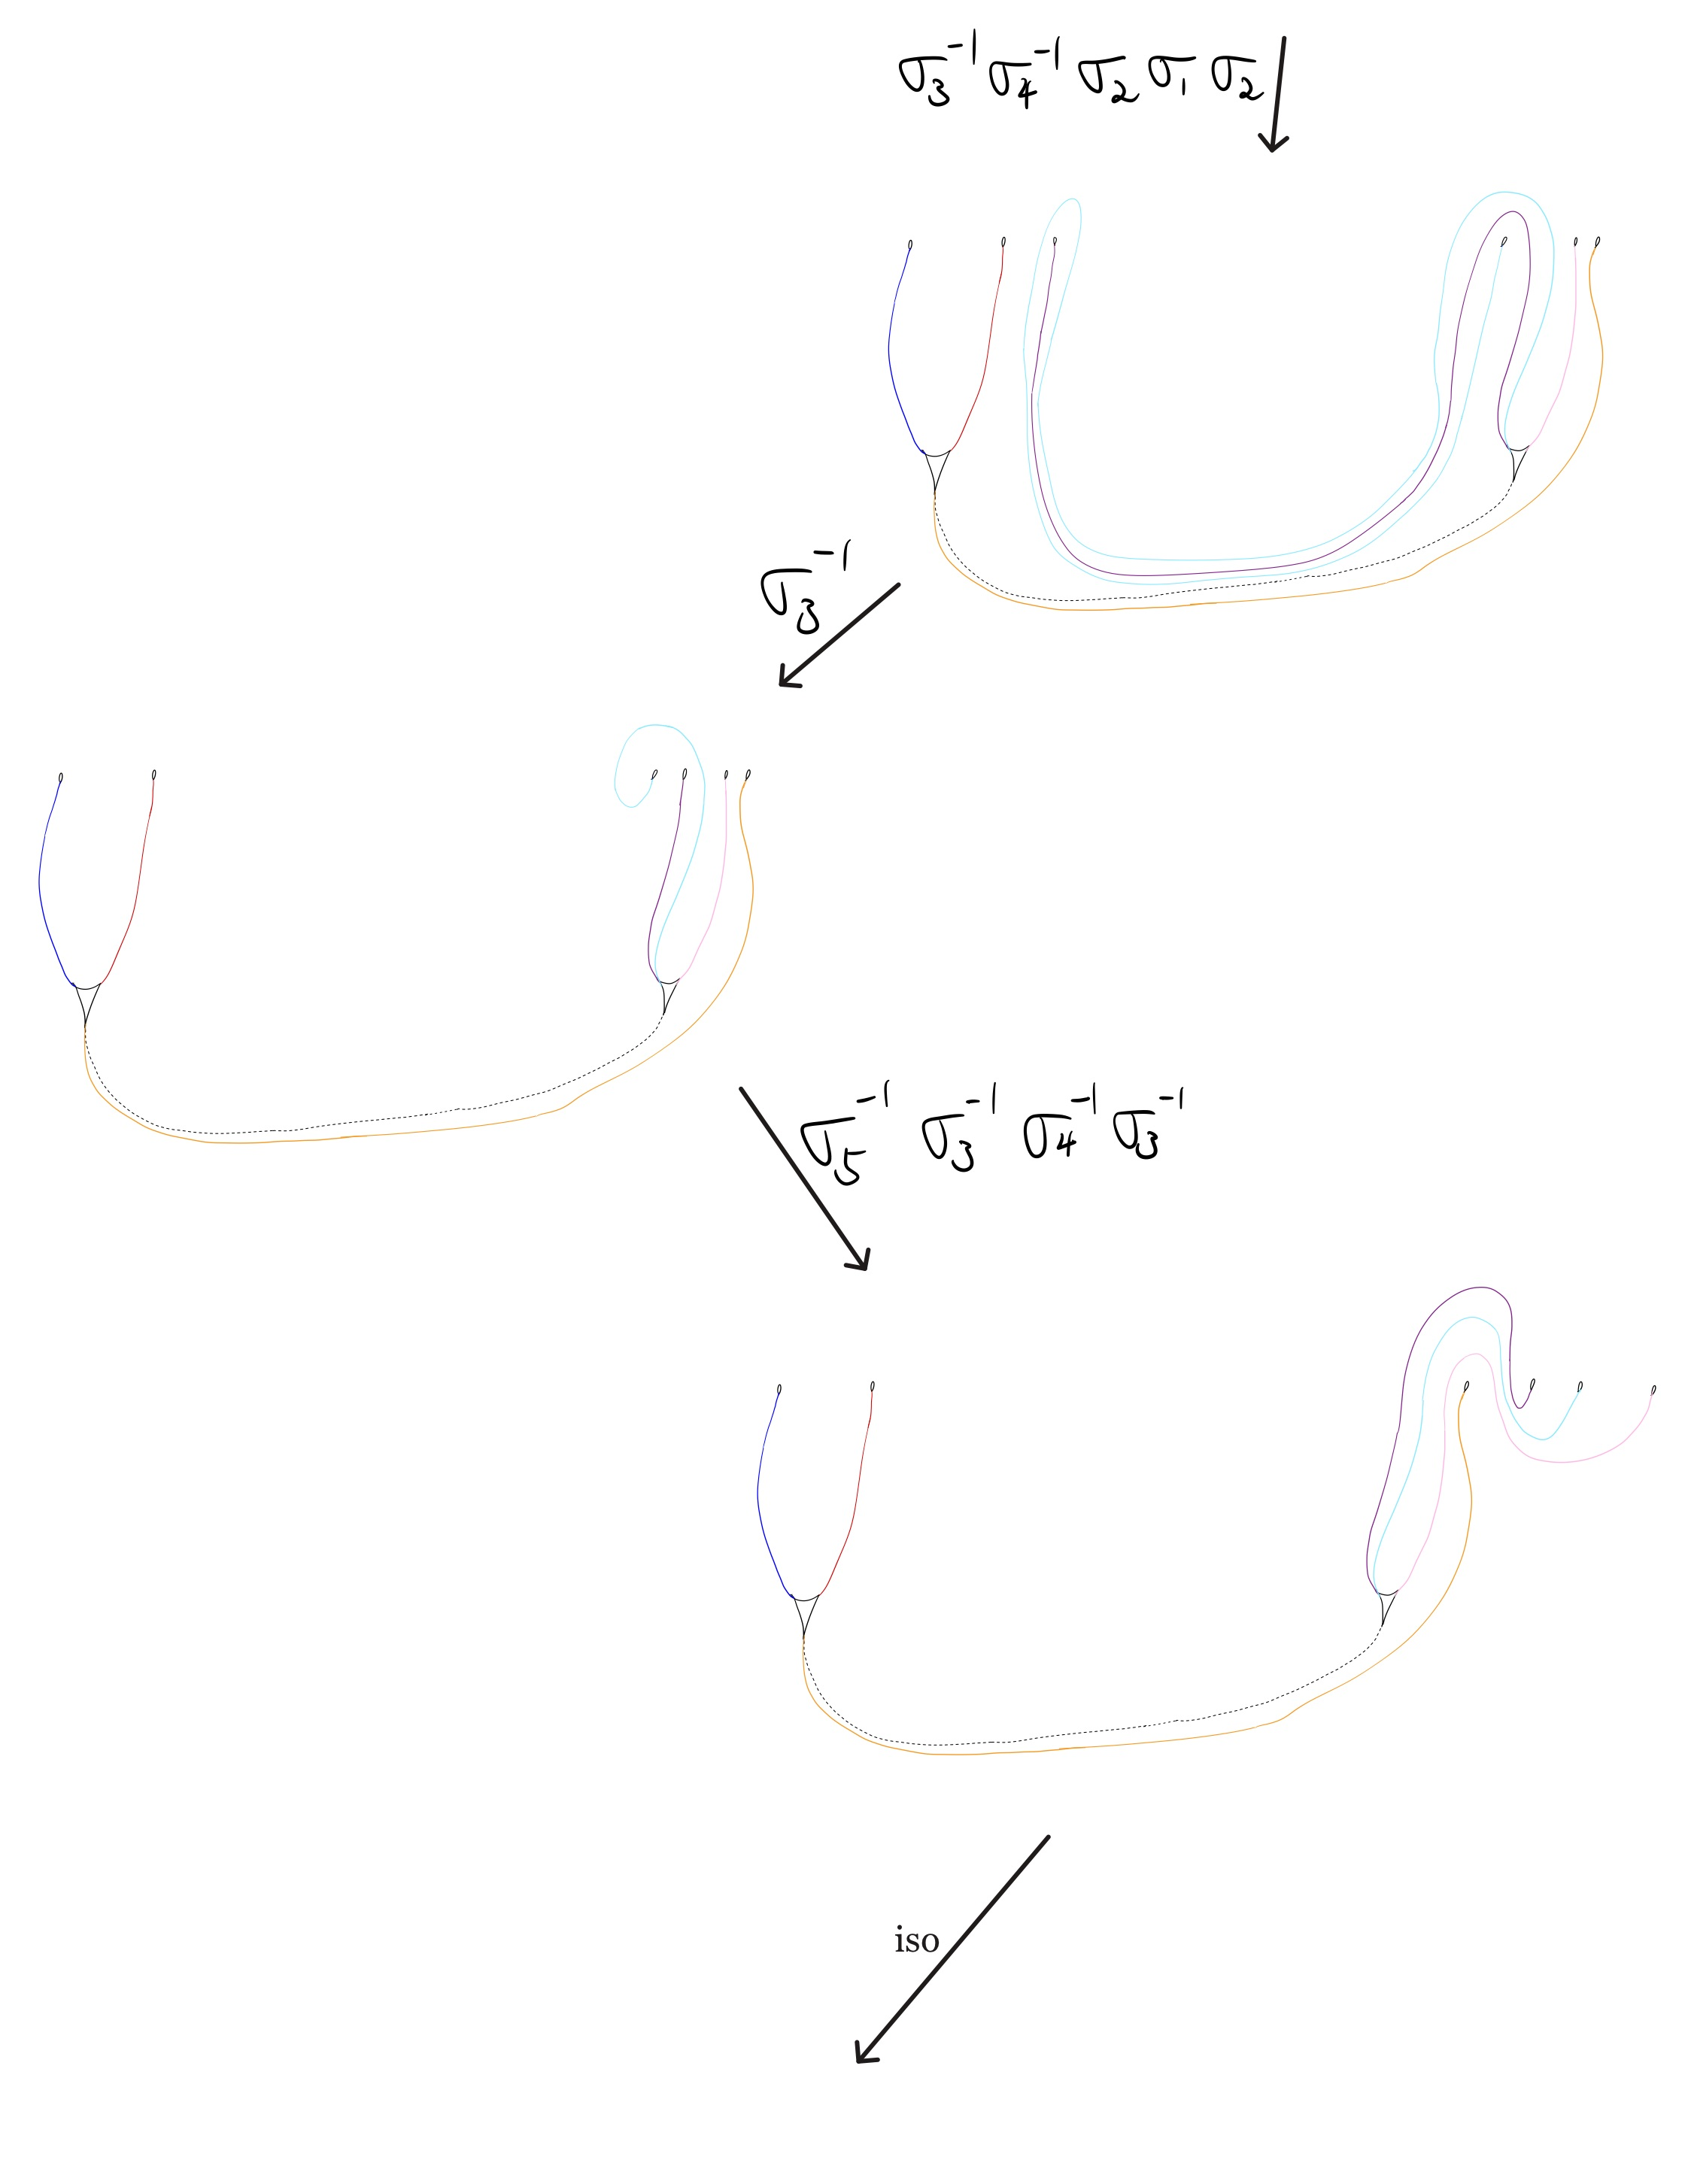
\includegraphics[width=\linewidth, height=0.45\textheight, keepaspectratio]{figures_braid/figures_track_8/Track 8 Braid 2 Diatree-3.jpg}
    \caption{This sequence shows the inverse of the braid $b_2^8$ carries Train Track Candidate Family 2.}
    \label{fig:track8_braid_b8_2}
\end{figure*}

\clearpage

\section{Candidate Family 3 (Fulmine)}\label{sec:track8_fulmine}
Train Track Map Candidate Family 3 of Track 8 is shown in Figure \ref{fig:track8_braid_b8_3_map}. See \ref{Fulmine} for details.

\begin{figure*}[ht]
    \centering
    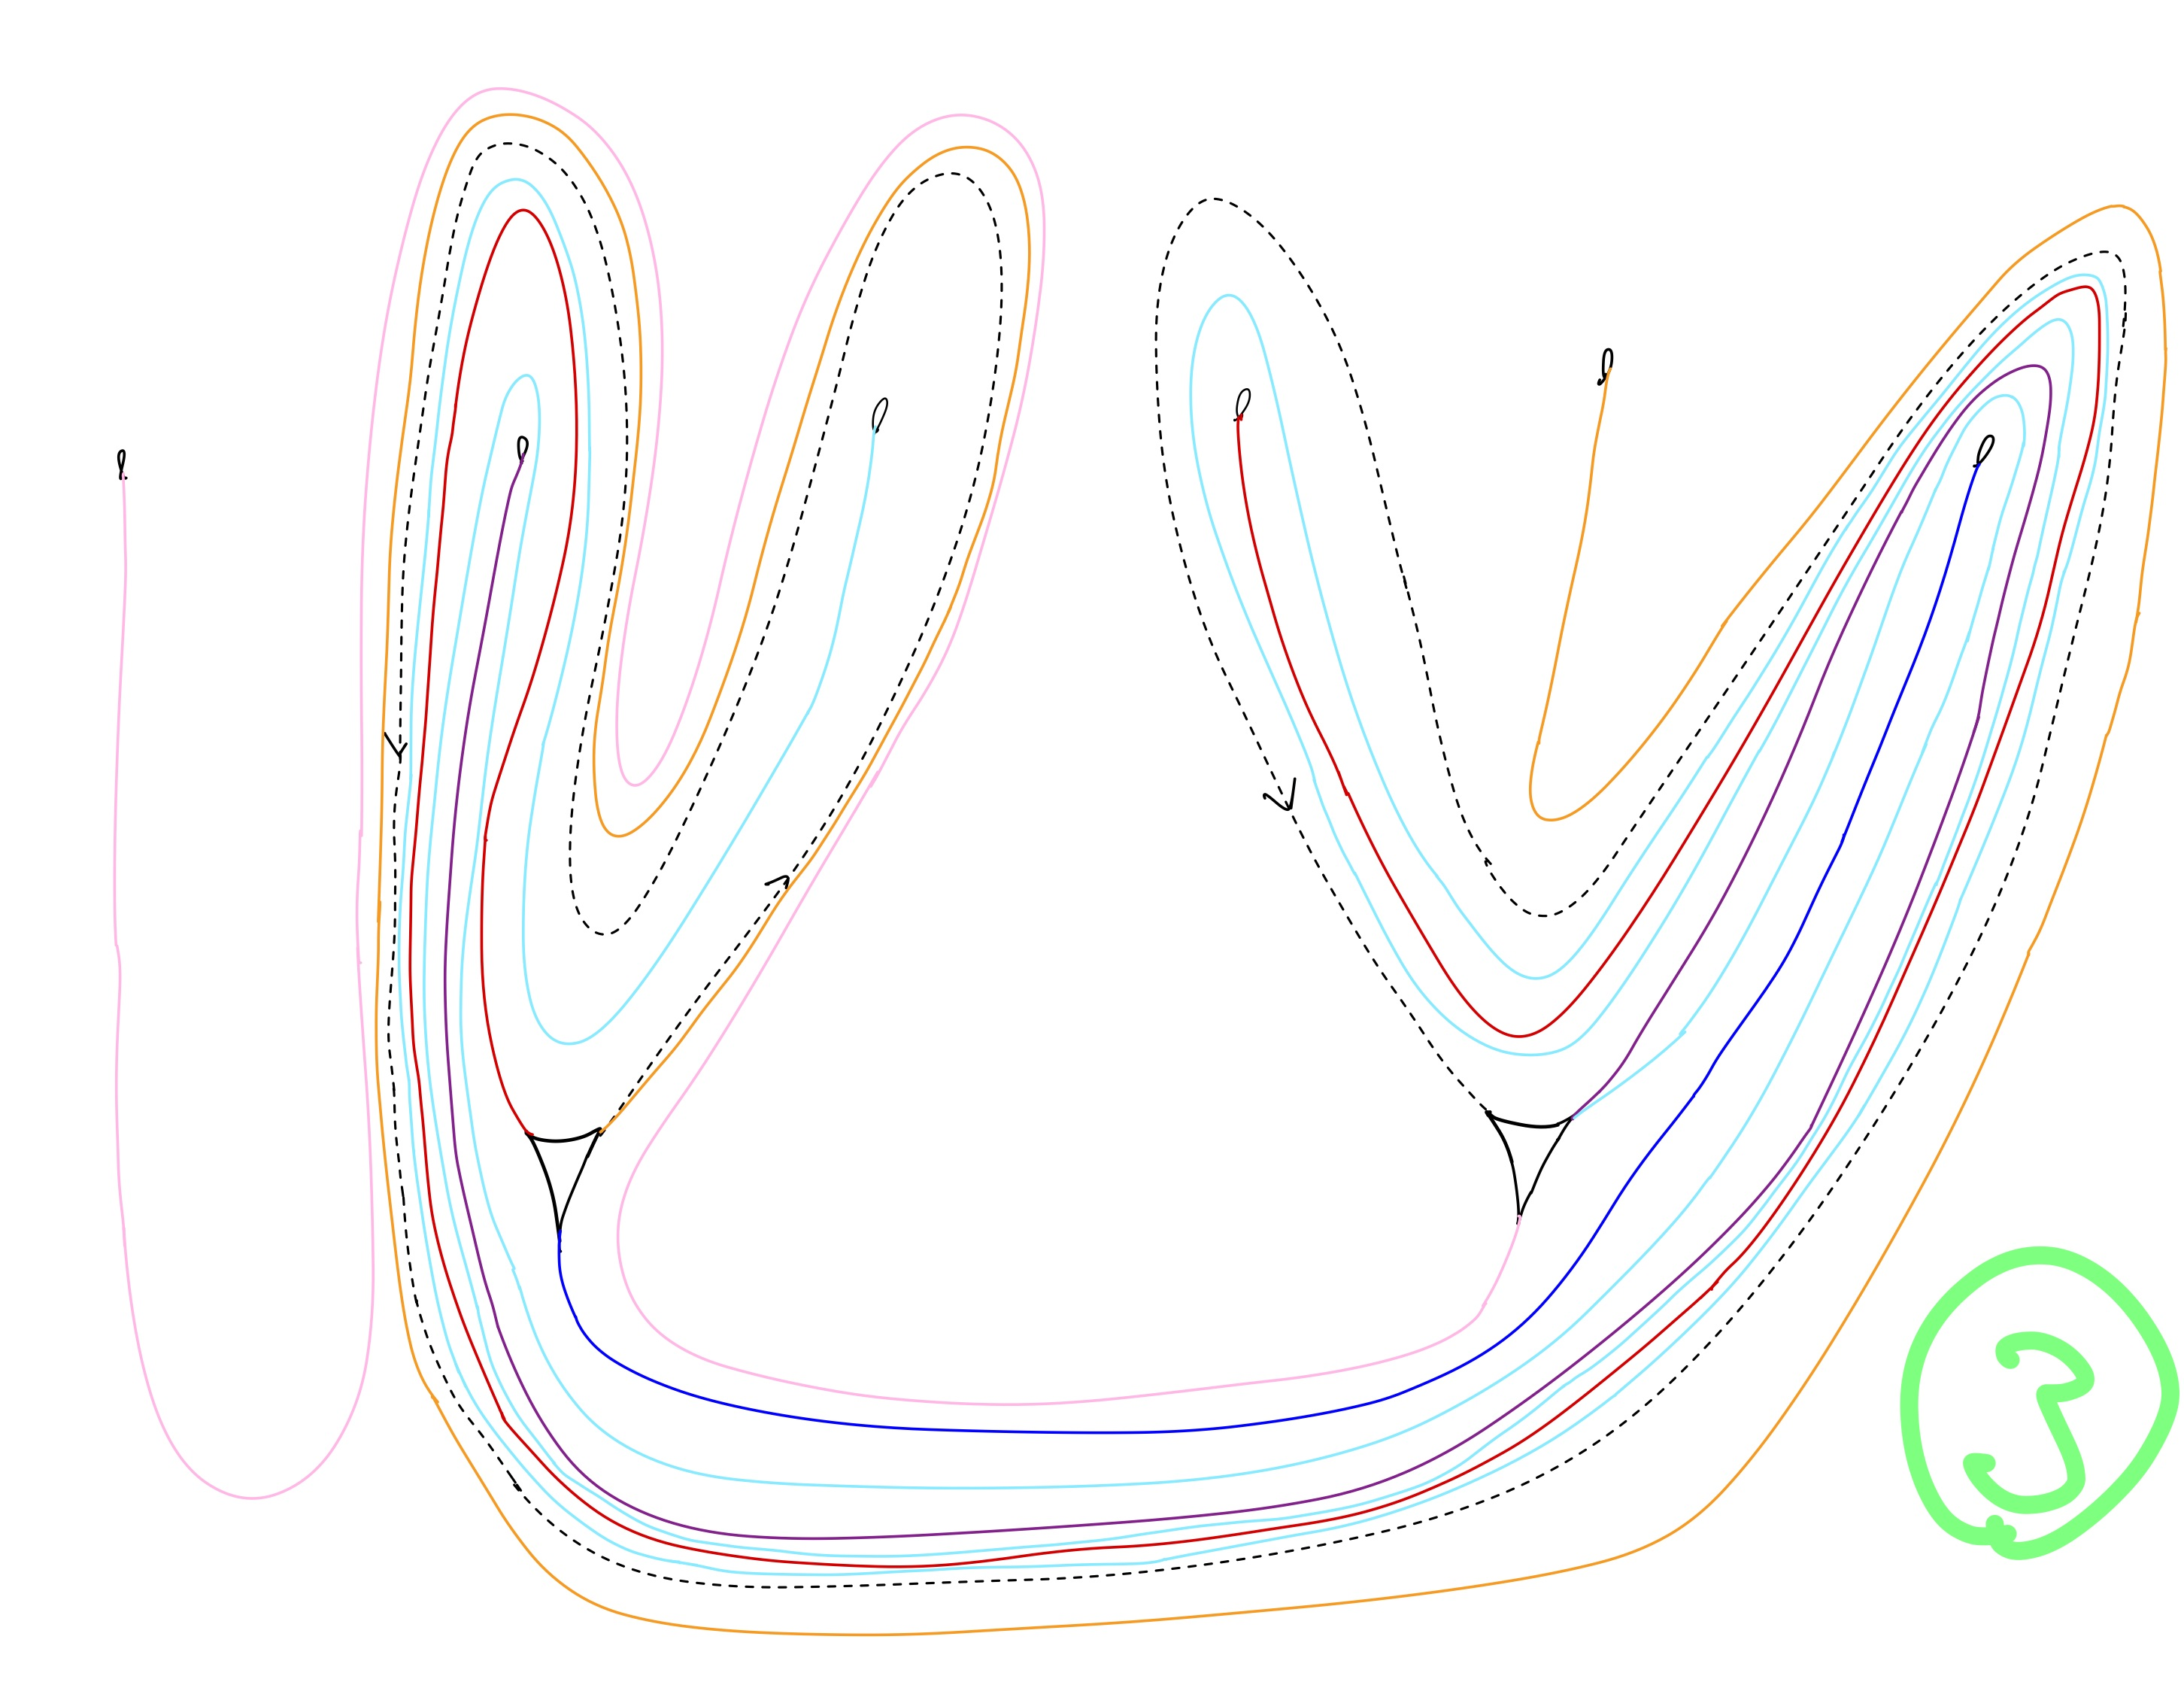
\includegraphics[width=\linewidth, height=0.45\textheight, keepaspectratio]{figures_braid/figures_track_8/Track 8 Braid 3 Fulmine-1.jpg}
    \caption{Train Track Map Candidate Family 3 (Fulmine) of Track 8.}
    \label{fig:track8_braid_b8_3_map}
\end{figure*}

The inverse of the following braid carries this family of train track maps:
\[
b_3^8 = \sigma_{5}^{-1} \sigma_{2} \sigma_{4}^{-1} \sigma_{1}^{-1} \sigma_{2}^{-1} \sigma_{3}^{-1} \sigma_{4}^{-1} \sigma_{5}^{-1} \sigma_{2} \sigma_{1} \sigma_{3}^{-1} \sigma_{4}^{-1} \sigma_{2} \sigma_{3}^{-1} \sigma_{4}^{-1} \sigma_{2}^{-1} \sigma_{1}^{-1}
\]

This is shown in Figure \ref{fig:track8_braid_b8_3}.

\begin{figure*}[p]
    \centering
    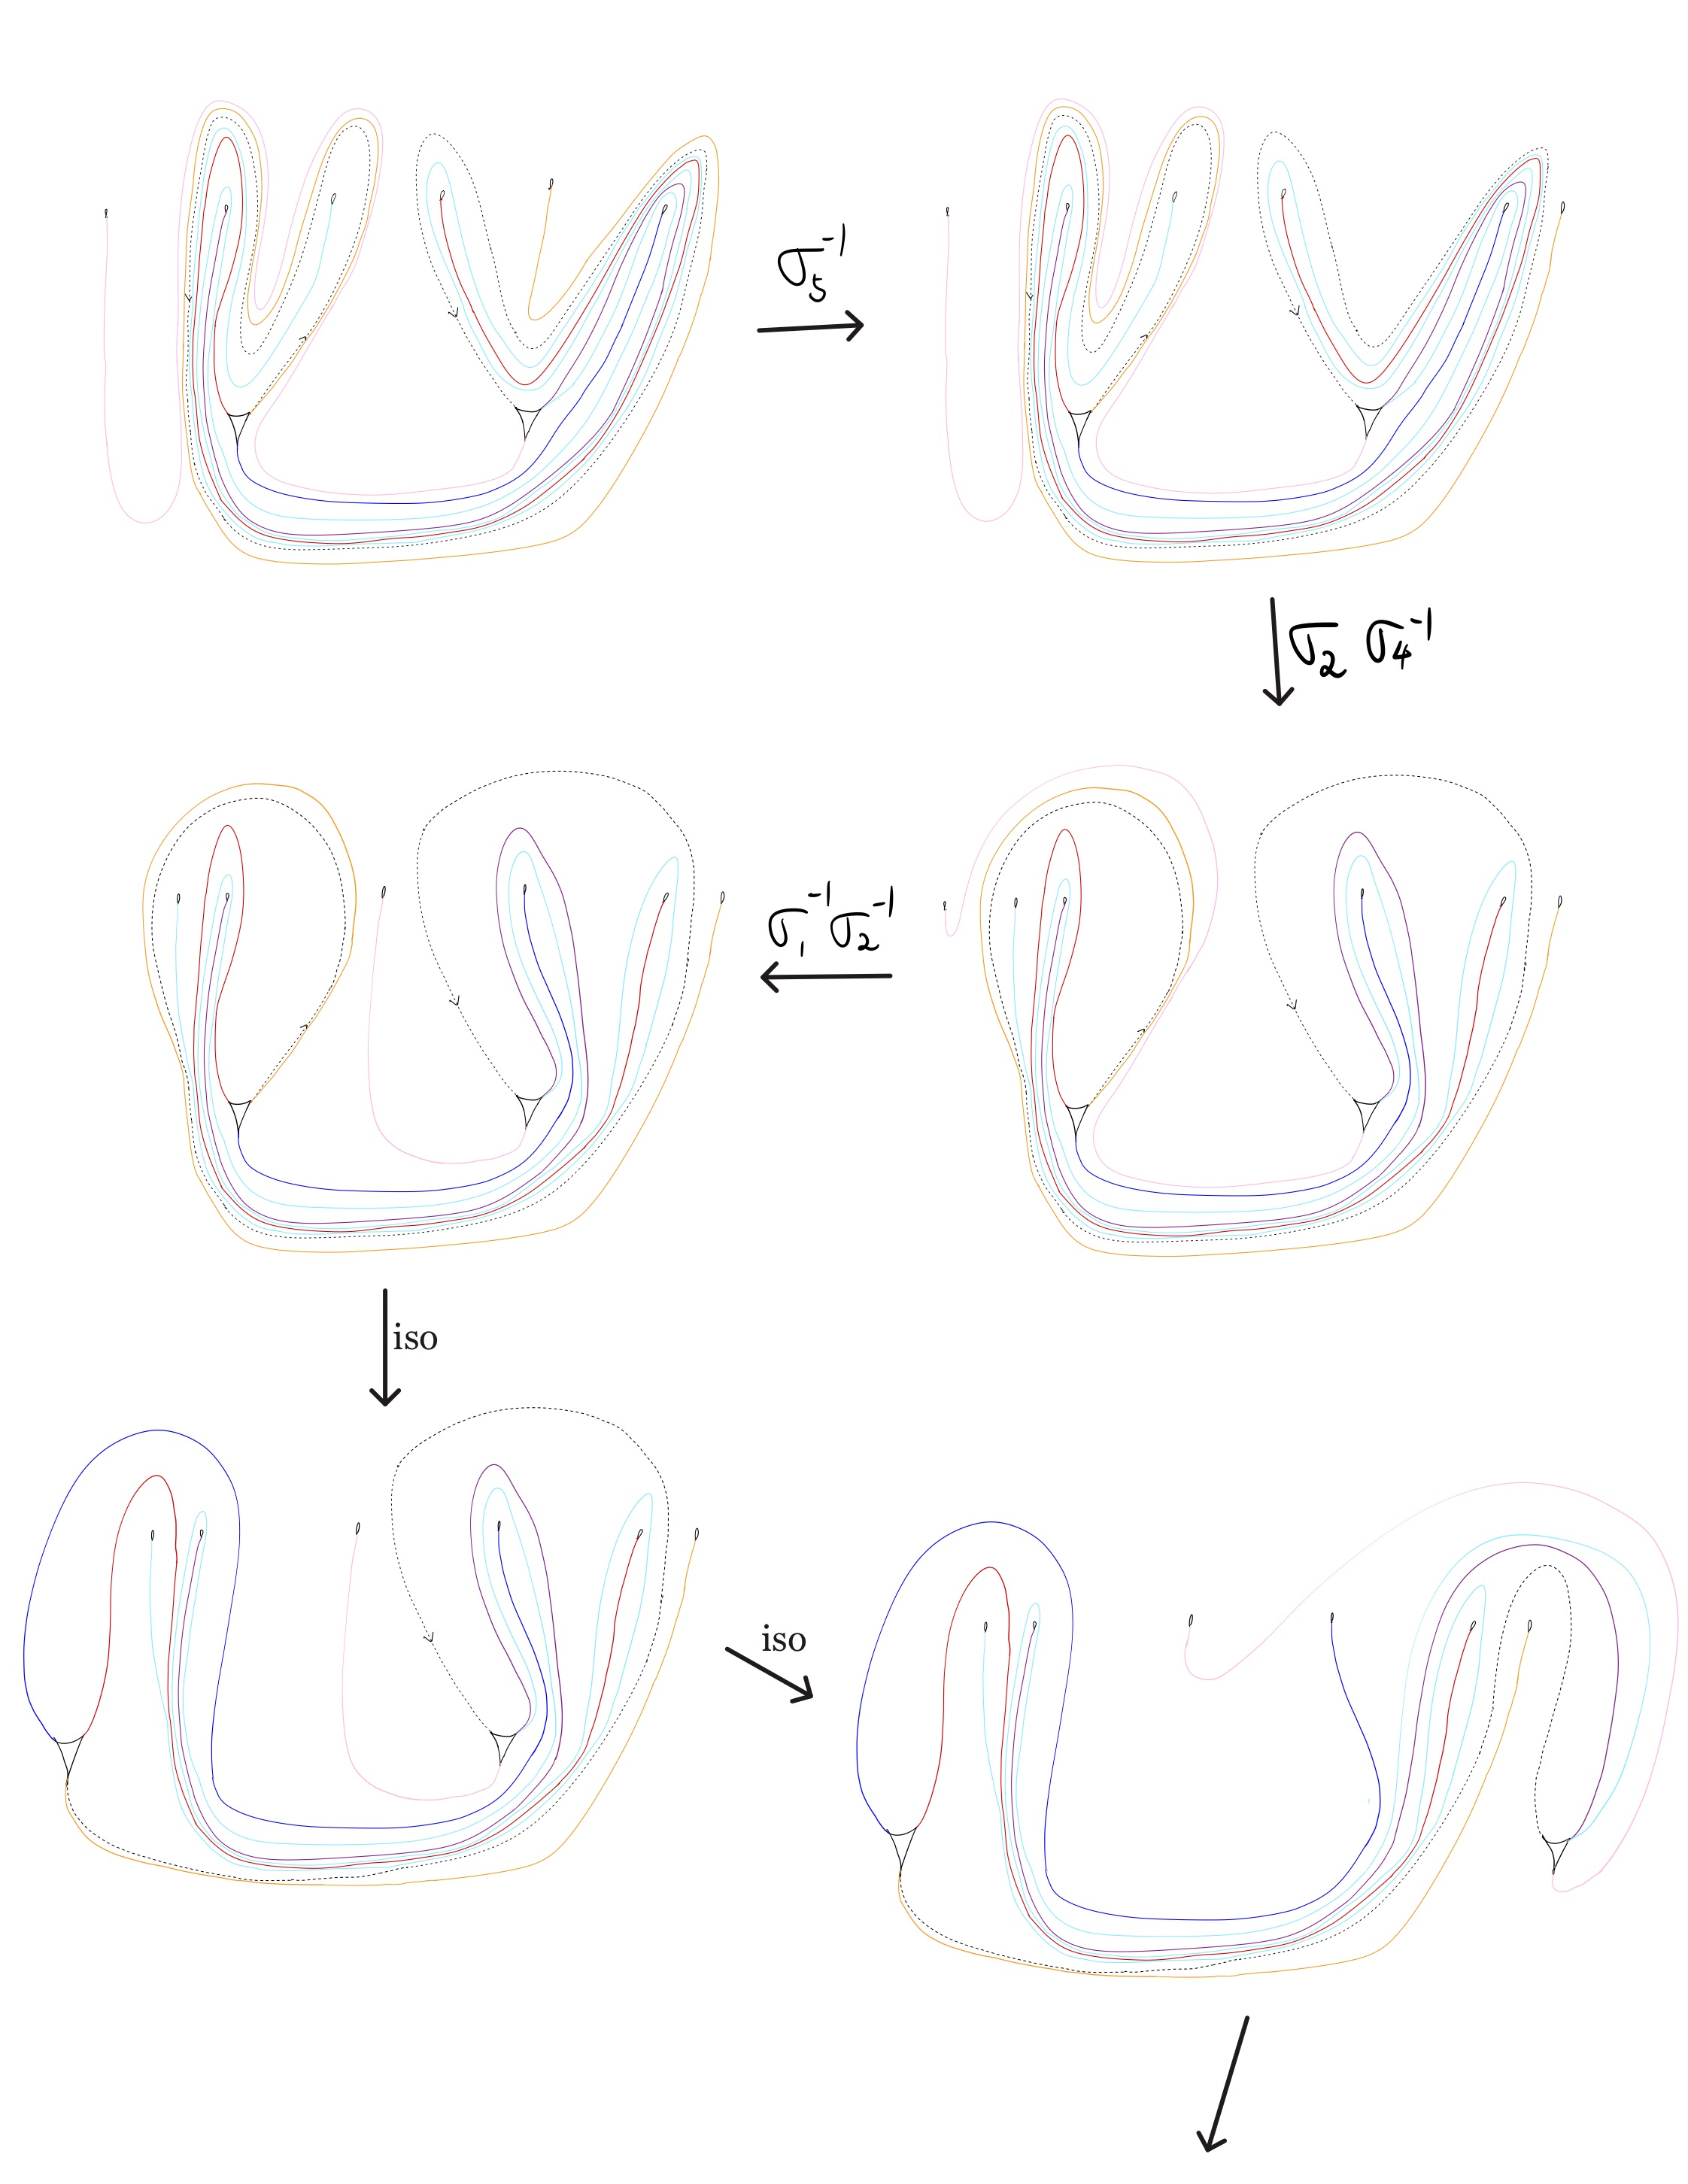
\includegraphics[width=\linewidth, height=0.45\textheight, keepaspectratio]{figures_braid/figures_track_8/Track 8 Braid 3 Fulmine-2.jpg}%
    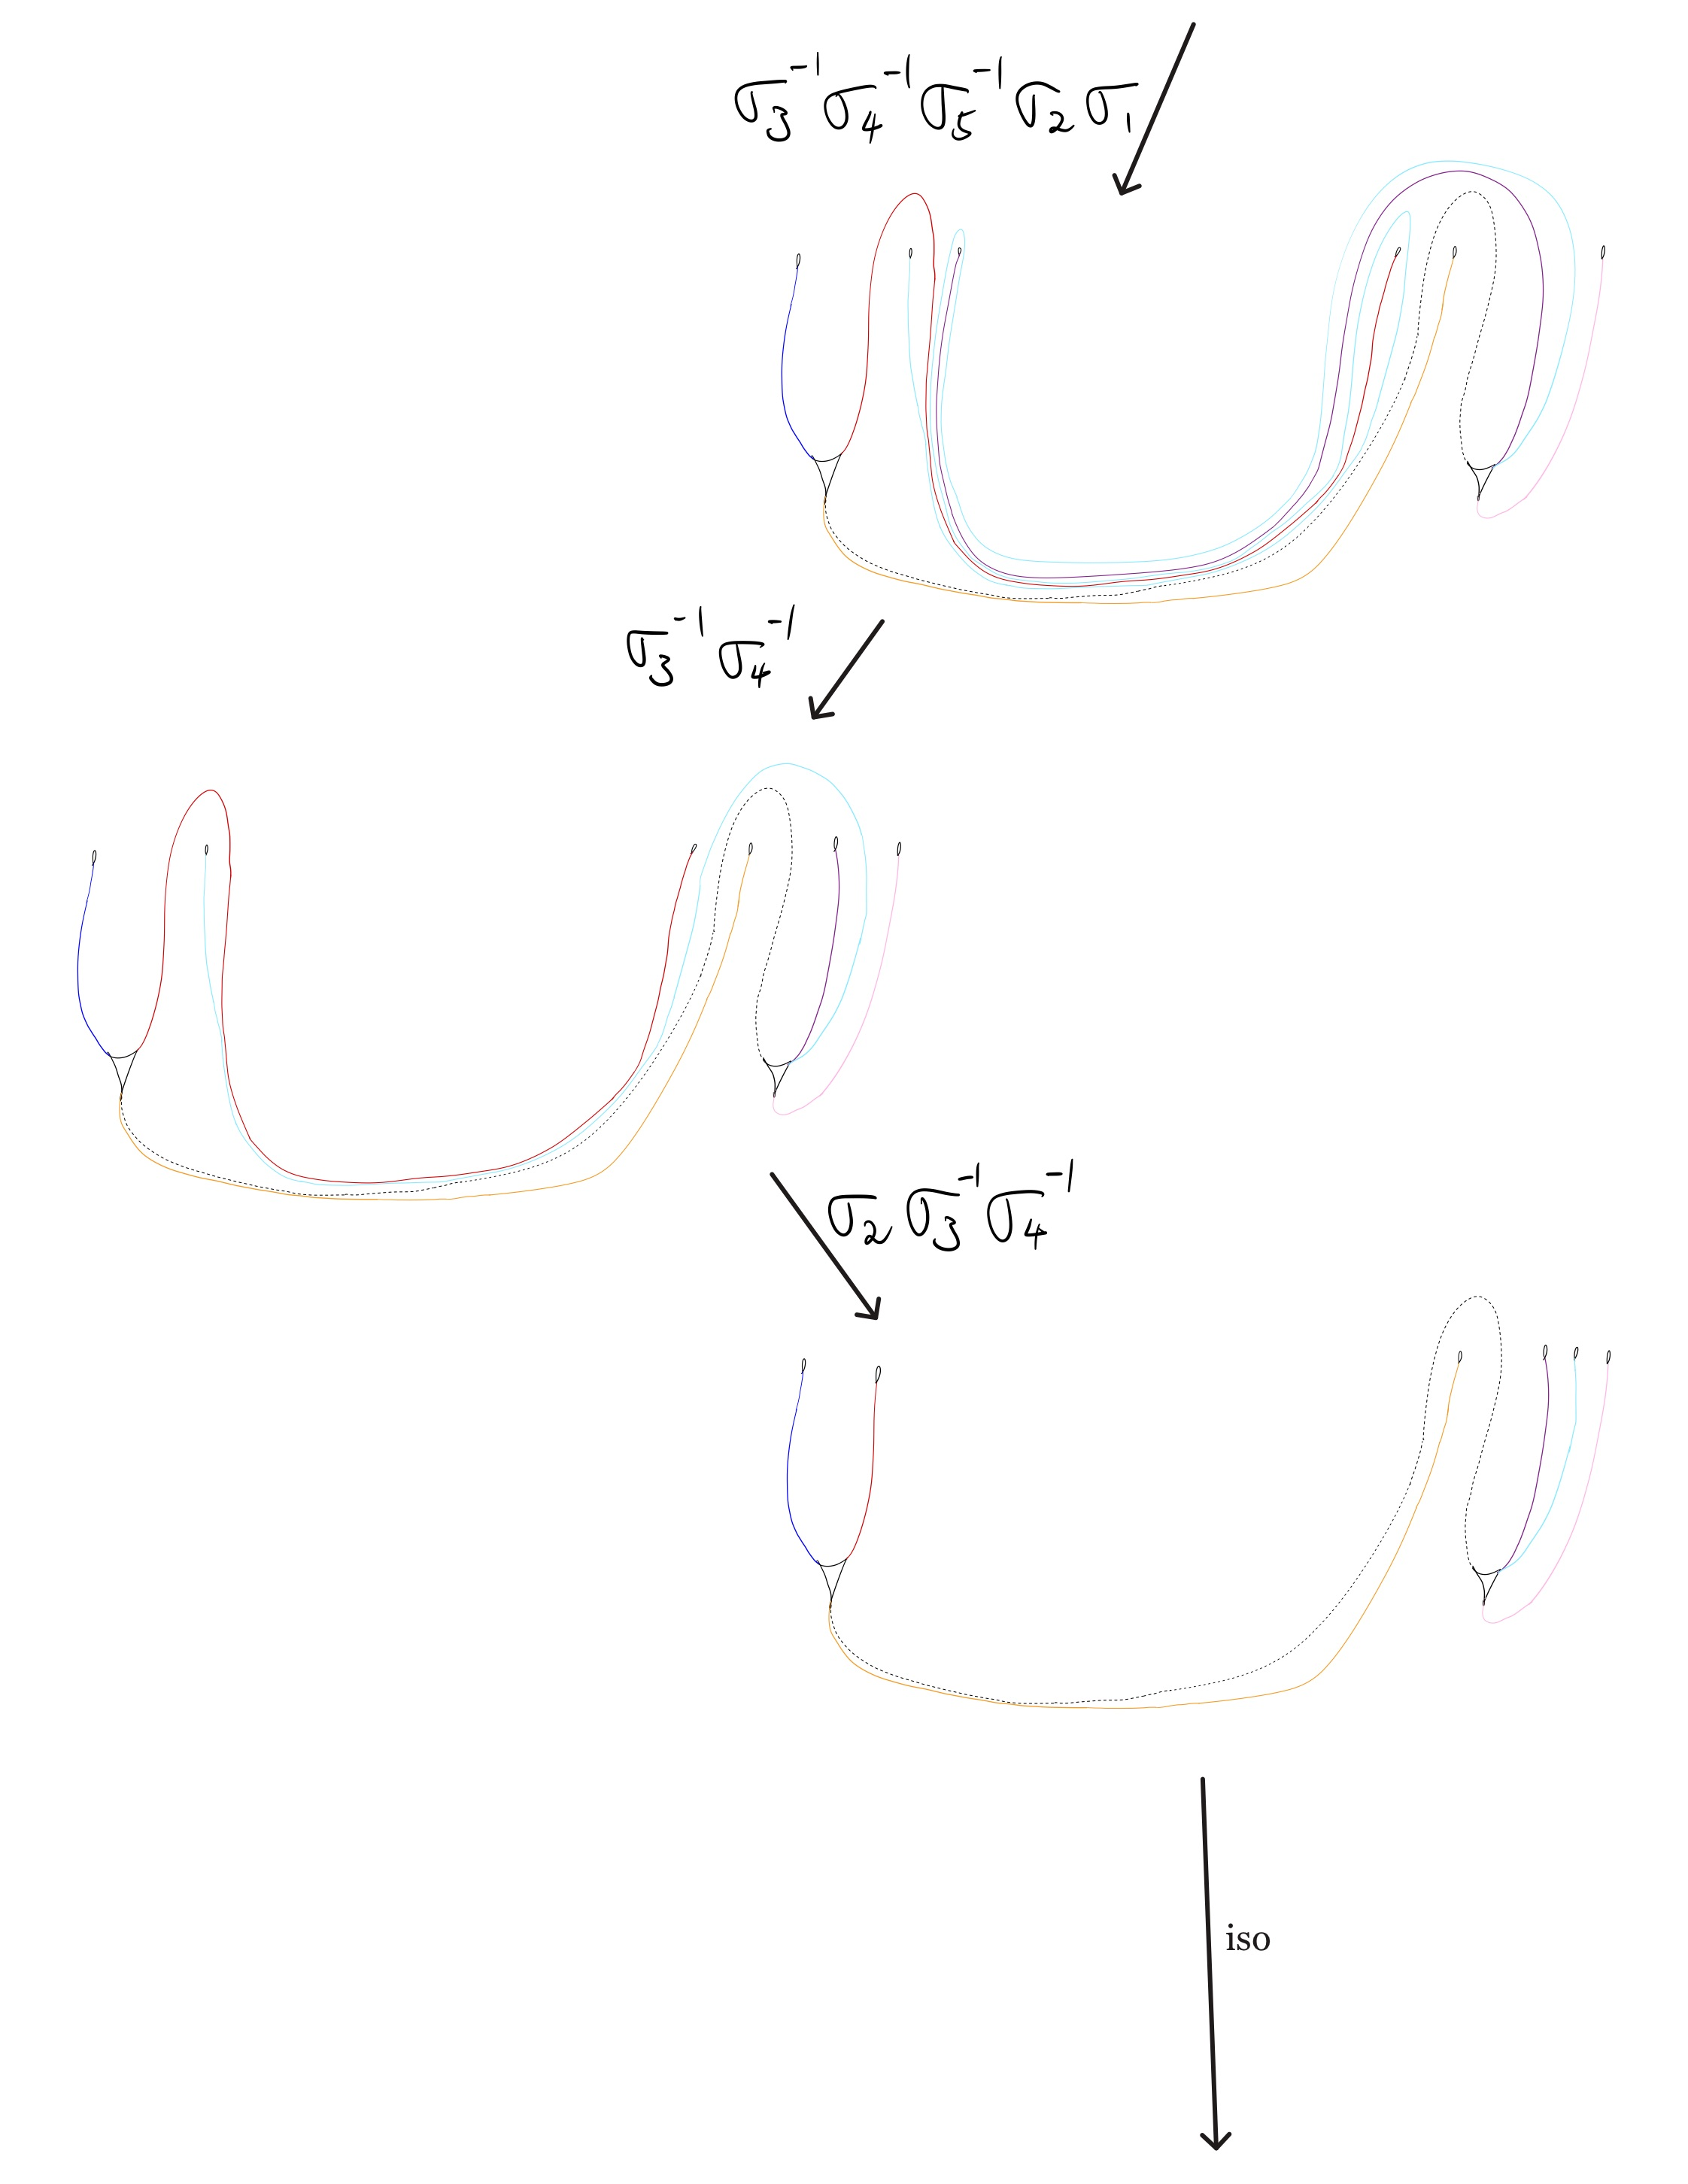
\includegraphics[width=\linewidth, height=0.45\textheight, keepaspectratio]{figures_braid/figures_track_8/Track 8 Braid 3 Fulmine-3.jpg}
    \caption{This sequence shows the inverse of the braid $b_3^8$ carries Train Track Candidate Family 3.}
    \label{fig:track8_braid_b8_3}
\end{figure*}

\clearpage

\section{Candidate Family 4 (Chine)}\label{sec:track8_chine}
Train Track Map Candidate Family 4 of Track 8 is shown in Figure \ref{fig:track8_braid_b8_4_map}. See \ref{Chine} for details.

\begin{figure*}[ht]
    \centering
    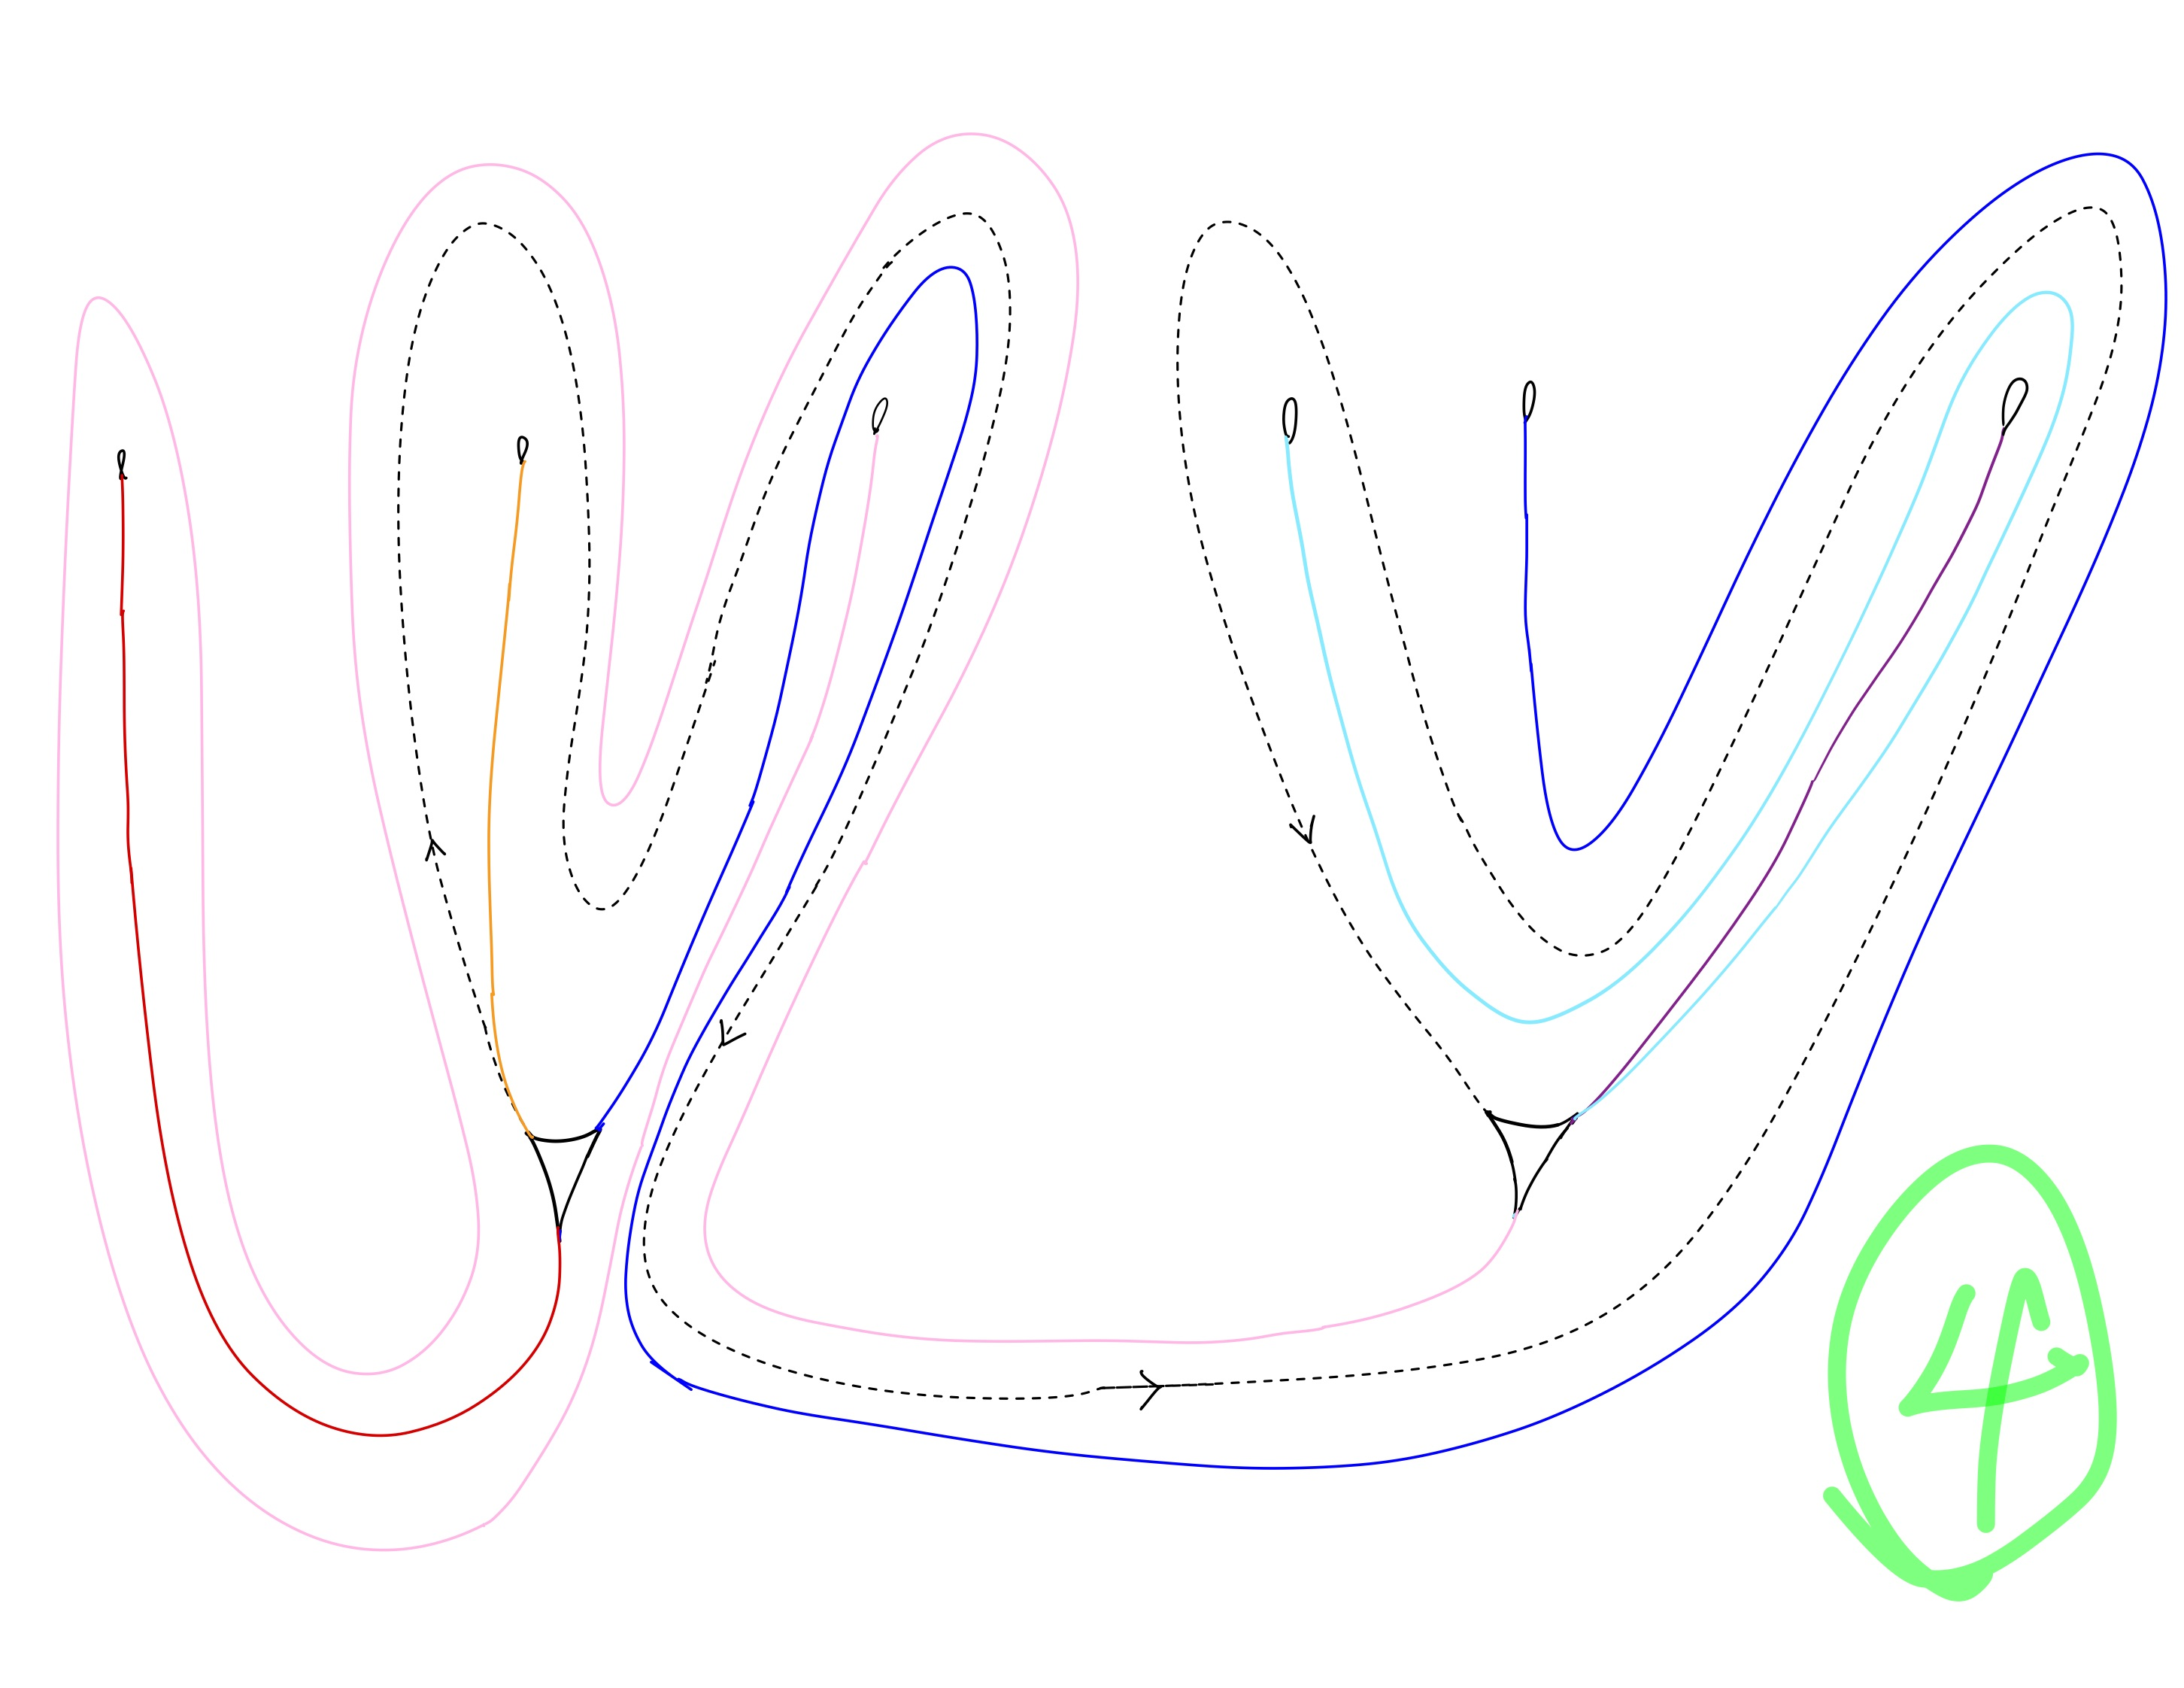
\includegraphics[width=\linewidth, height=0.45\textheight, keepaspectratio]{figures_braid/figures_track_8/Track 8 Braid 4 Chine-1.jpg}
    \caption{Train Track Map Candidate Family 4 (Chine) of Track 8.}
    \label{fig:track8_braid_b8_4_map}
\end{figure*}

The inverse of the following braid carries this family of train track maps:
\[
b_4^8 = \sigma_{5}^{-1} \sigma_{2}^{-1} \sigma_{1}^{-1} \sigma_{1}^{-1} \sigma_{2}^{-1} \sigma_{3}^{-1} \sigma_{4}^{-1} \sigma_{3}^{-1} \sigma_{3}^{-1} \sigma_{3}^{-1} \sigma_{5}^{-1} \sigma_{4}^{-1} \sigma_{3}^{-1} \sigma_{1}^{-1} \sigma_{2}^{-1} \sigma_{1}^{-1} \sigma_{1}^{-1}
\]

This is shown in Figure \ref{fig:track8_braid_b8_4}.

\begin{figure*}[p]
    \centering
    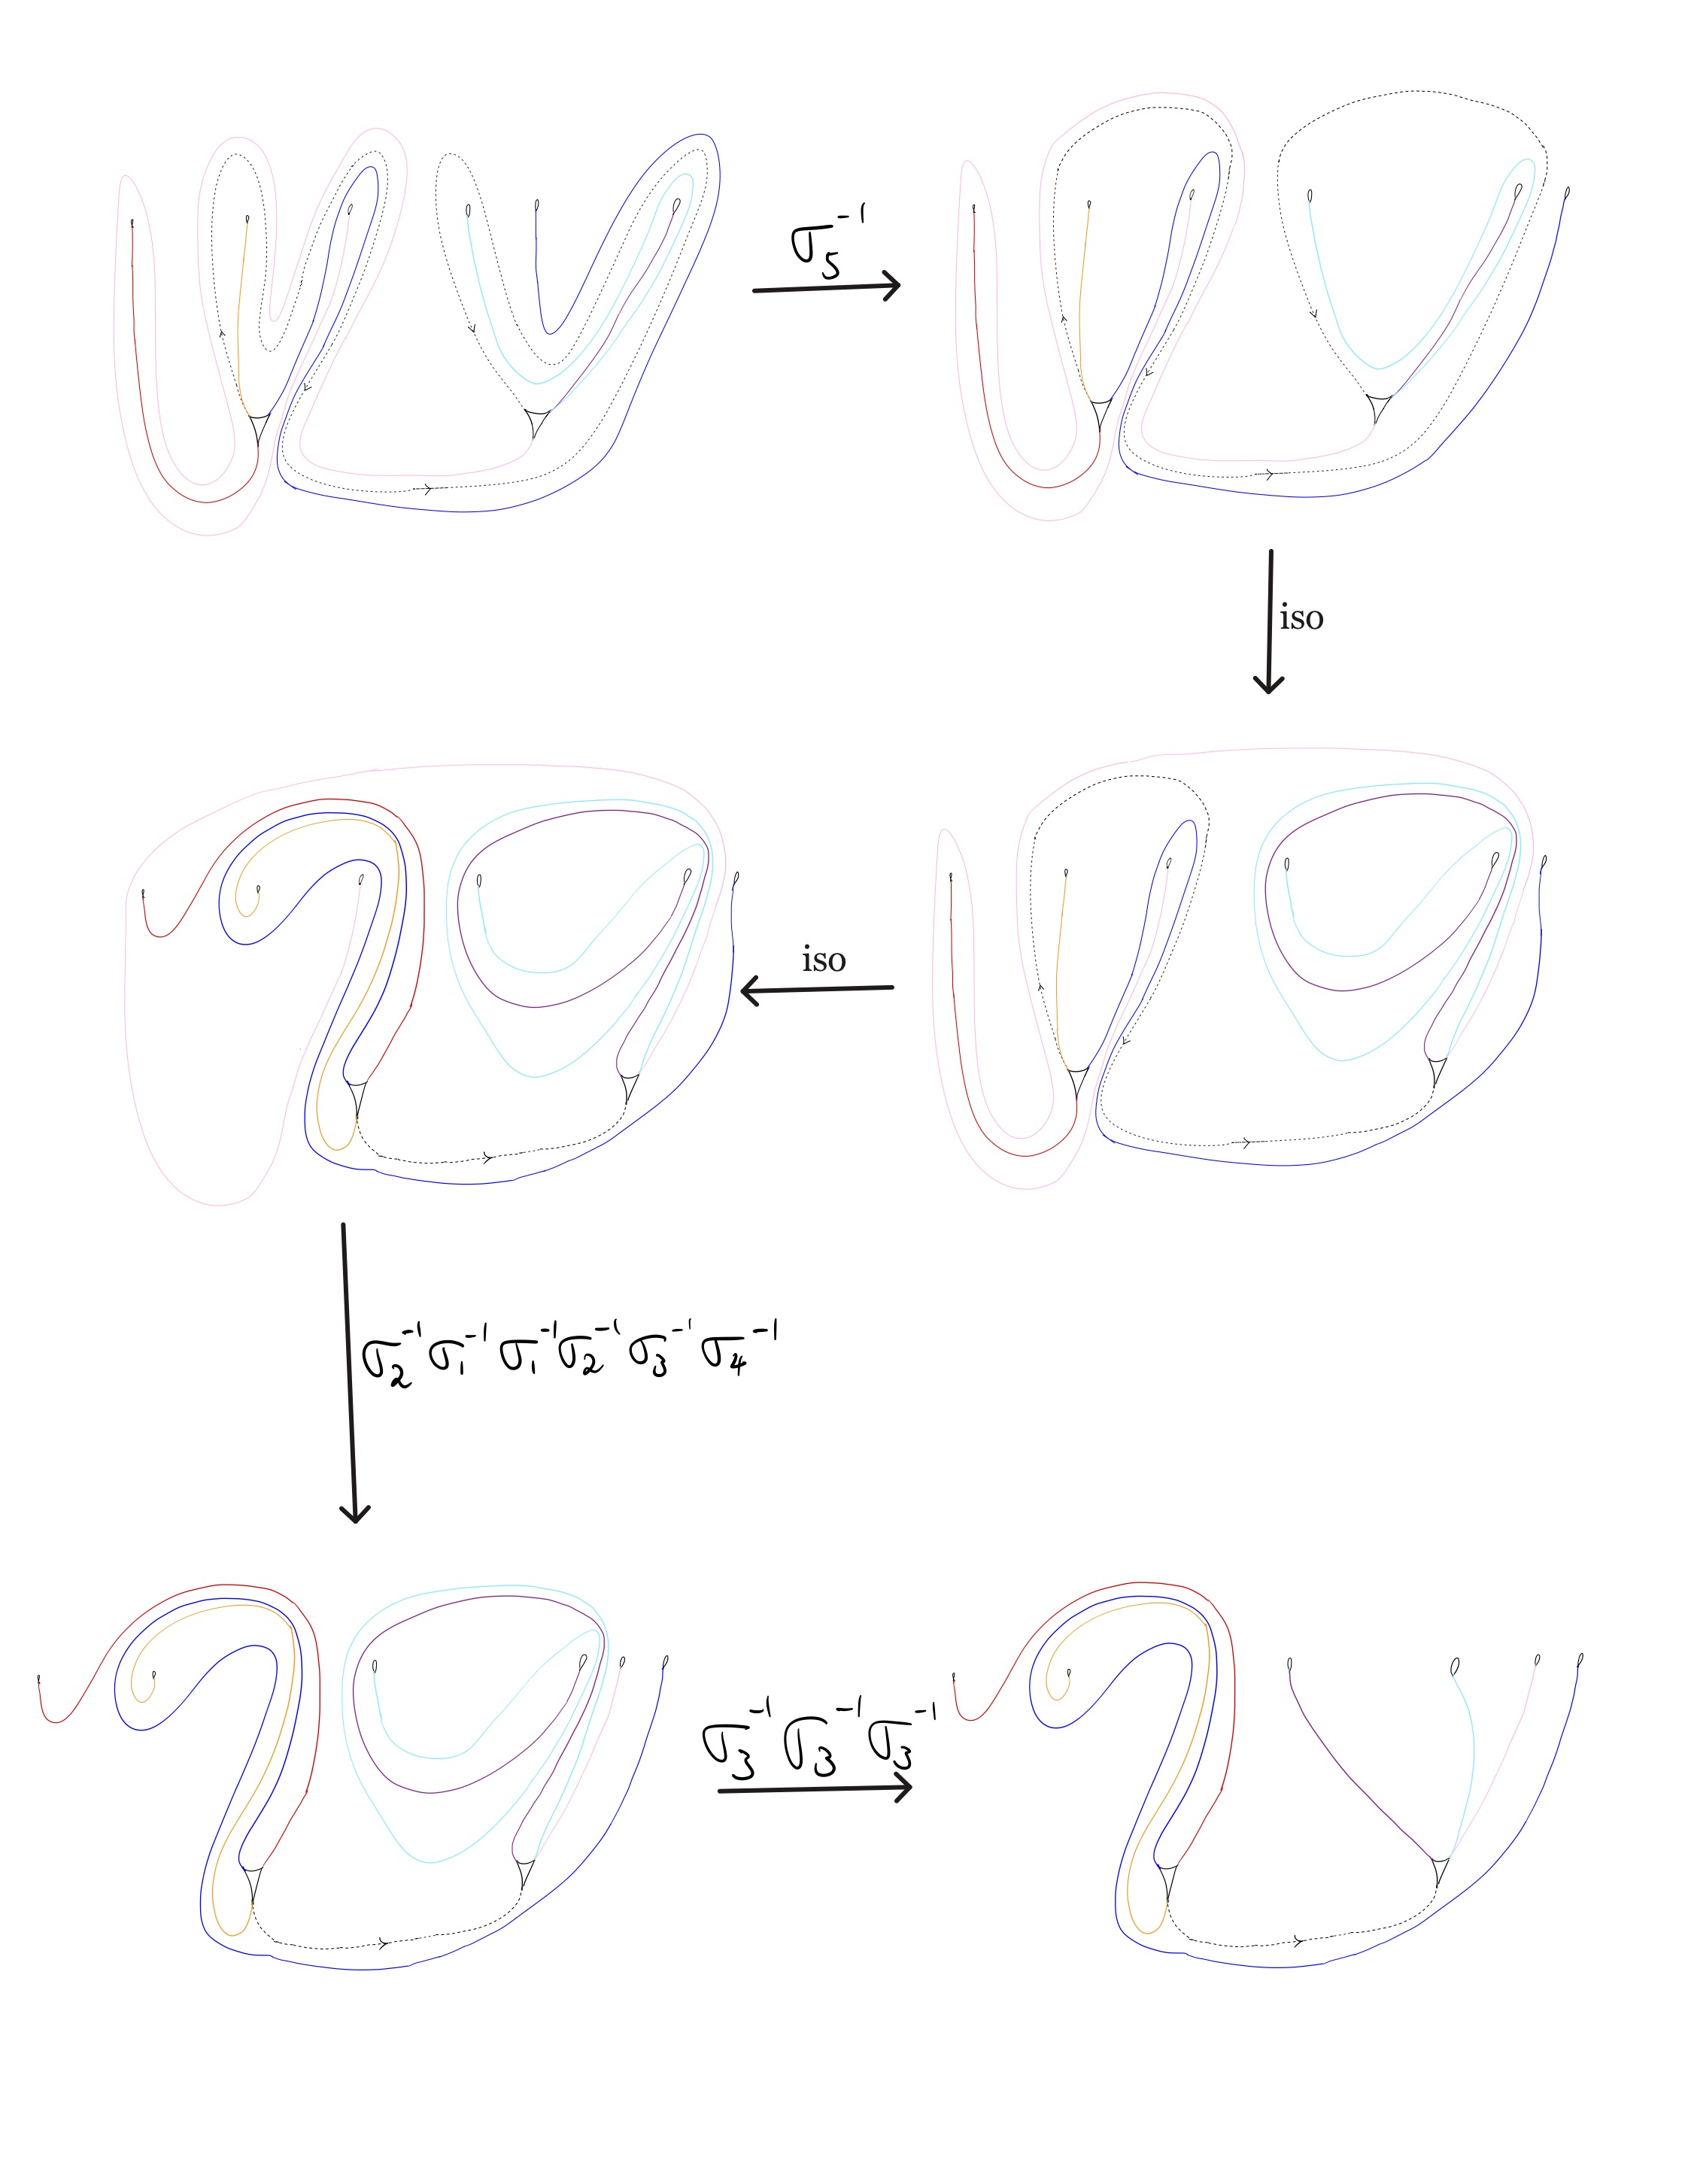
\includegraphics[width=\linewidth, height=0.45\textheight, keepaspectratio]{figures_braid/figures_track_8/Track 8 Braid 4 Chine-2.jpg}%
    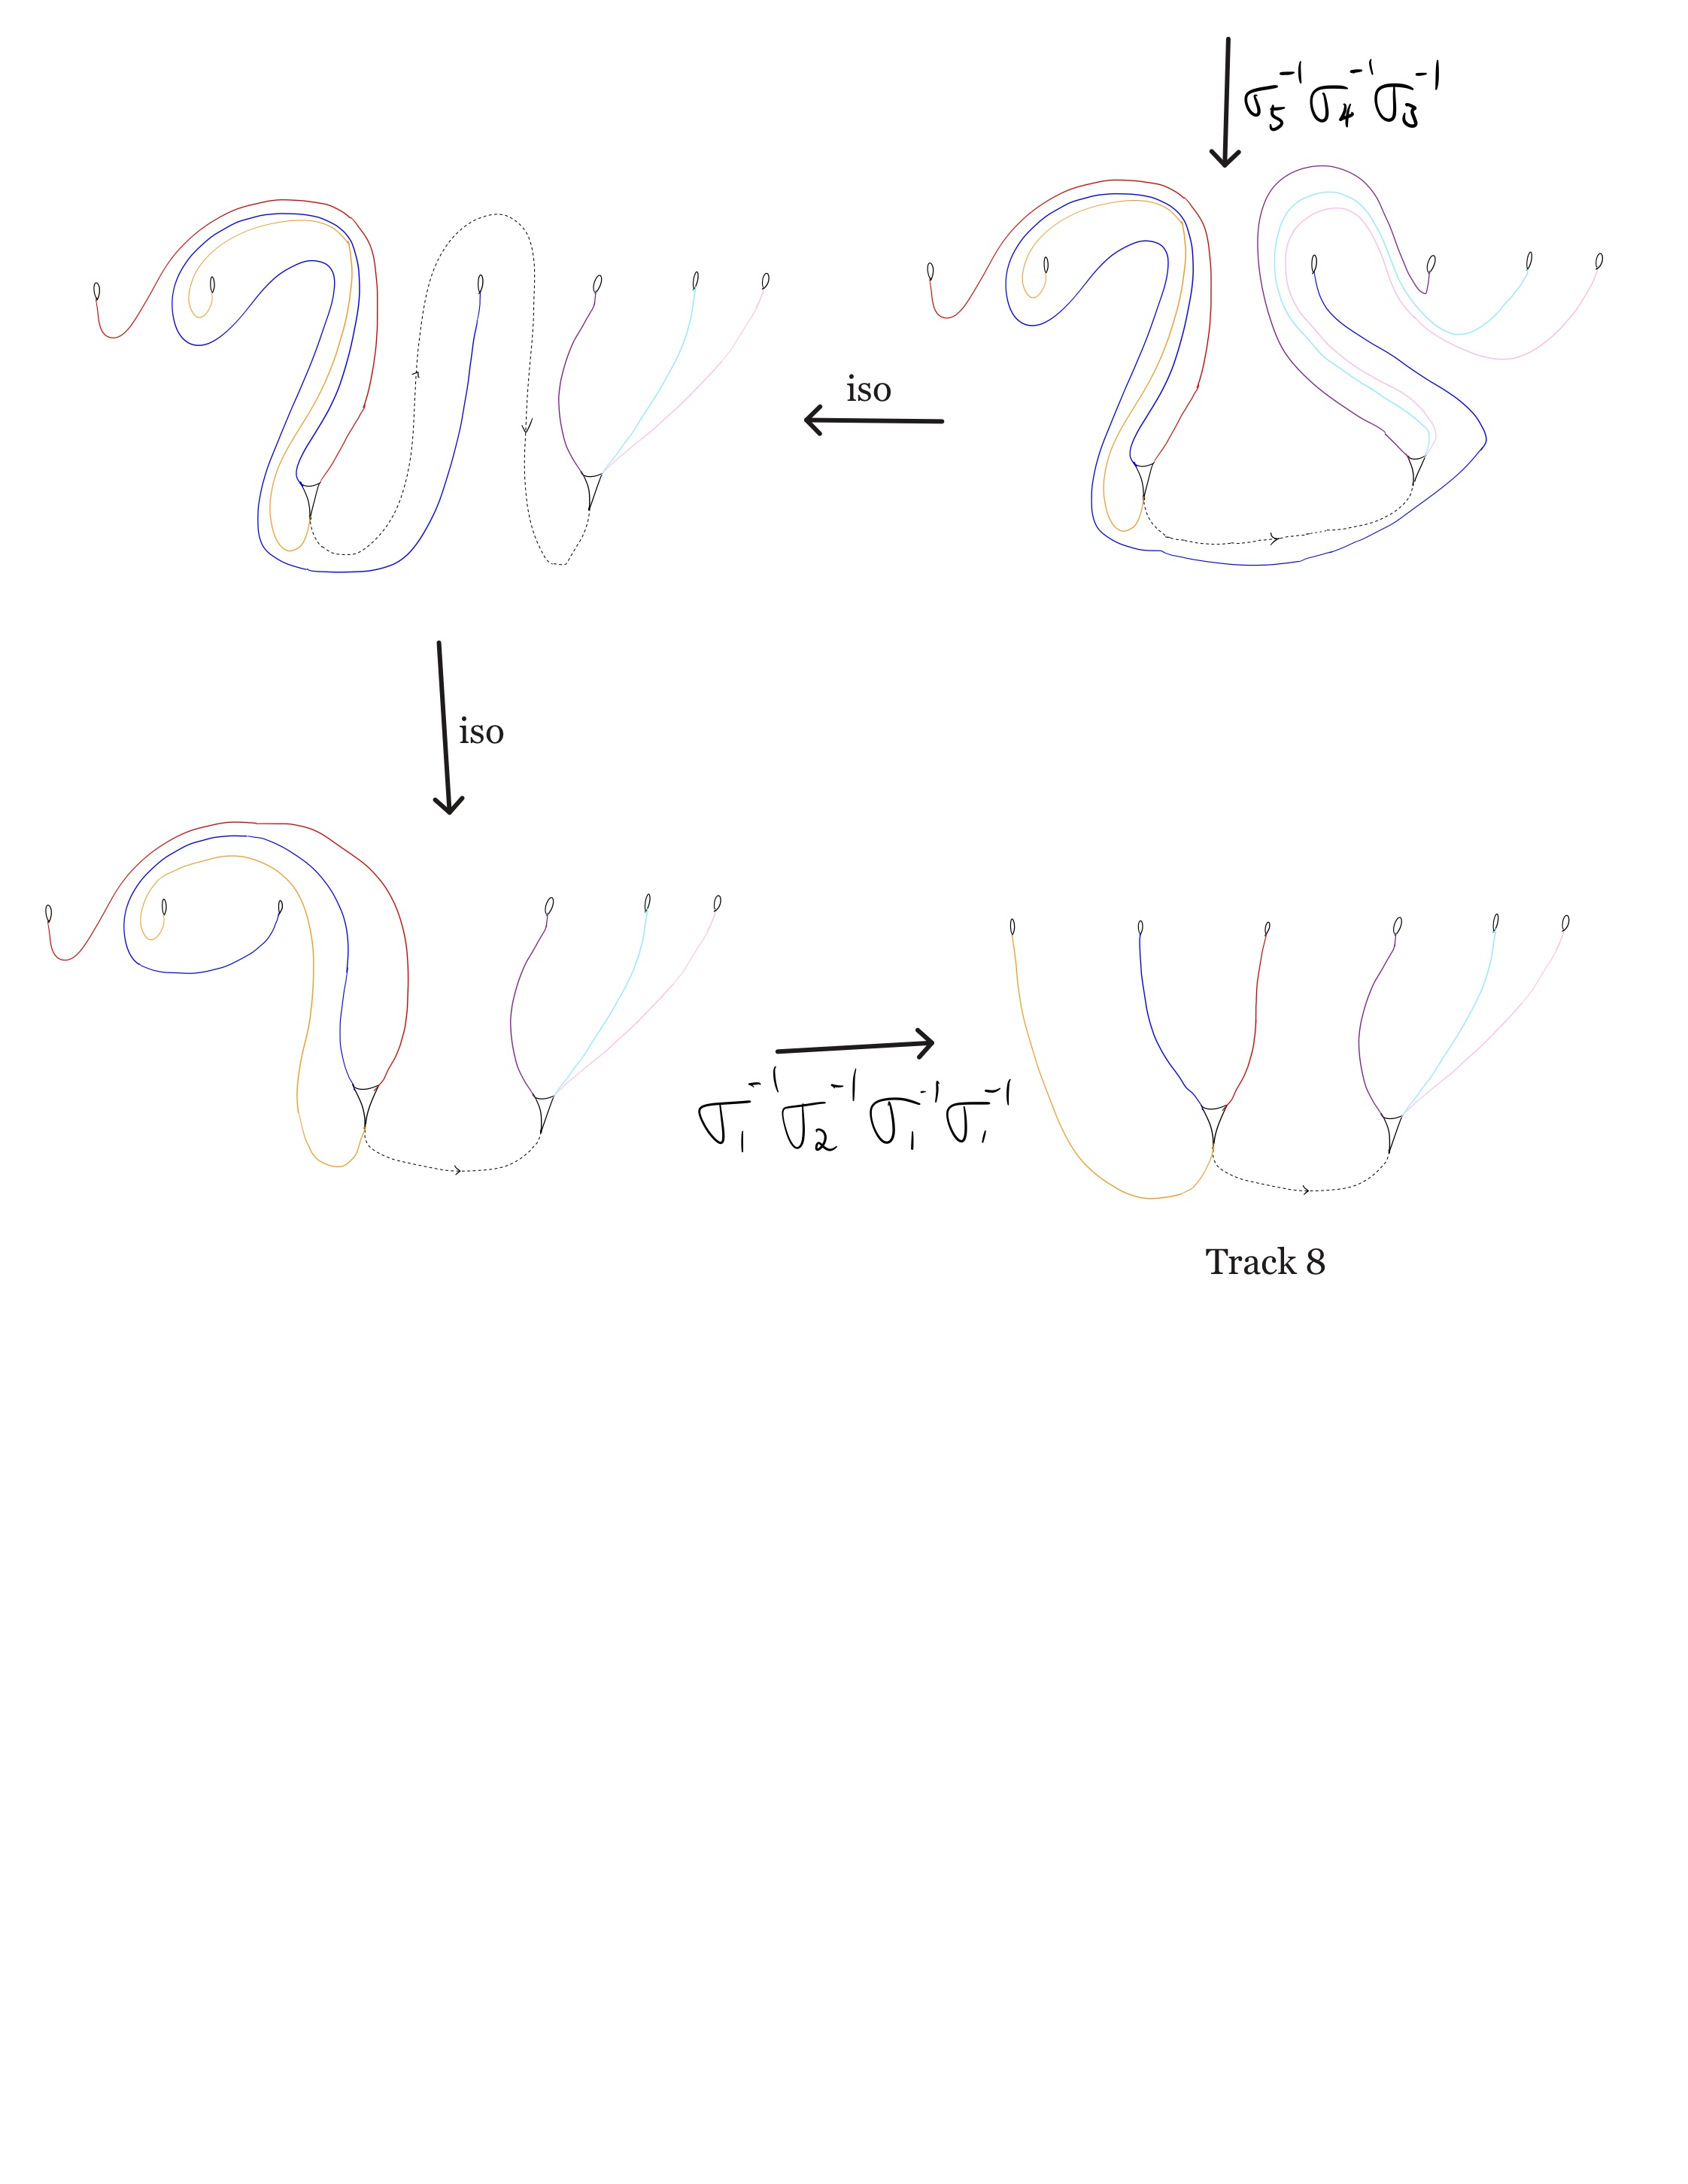
\includegraphics[width=\linewidth, height=0.45\textheight, keepaspectratio]{figures_braid/figures_track_8/Track 8 Braid 4 Chine-3.jpg}
    \caption{This sequence shows the inverse of the braid $b_4^8$ carries Train Track Candidate Family 4.}
    \label{fig:track8_braid_b8_4}
\end{figure*}

\clearpage

\section{Candidate Family 5 (Quaint)}\label{sec:track8_quaint}
Train Track Map Candidate Family 5 of Track 8 is shown in Figure \ref{fig:track8_braid_b8_5_map}. See \ref{Quaint} for details.

\begin{figure*}[ht]
    \centering
    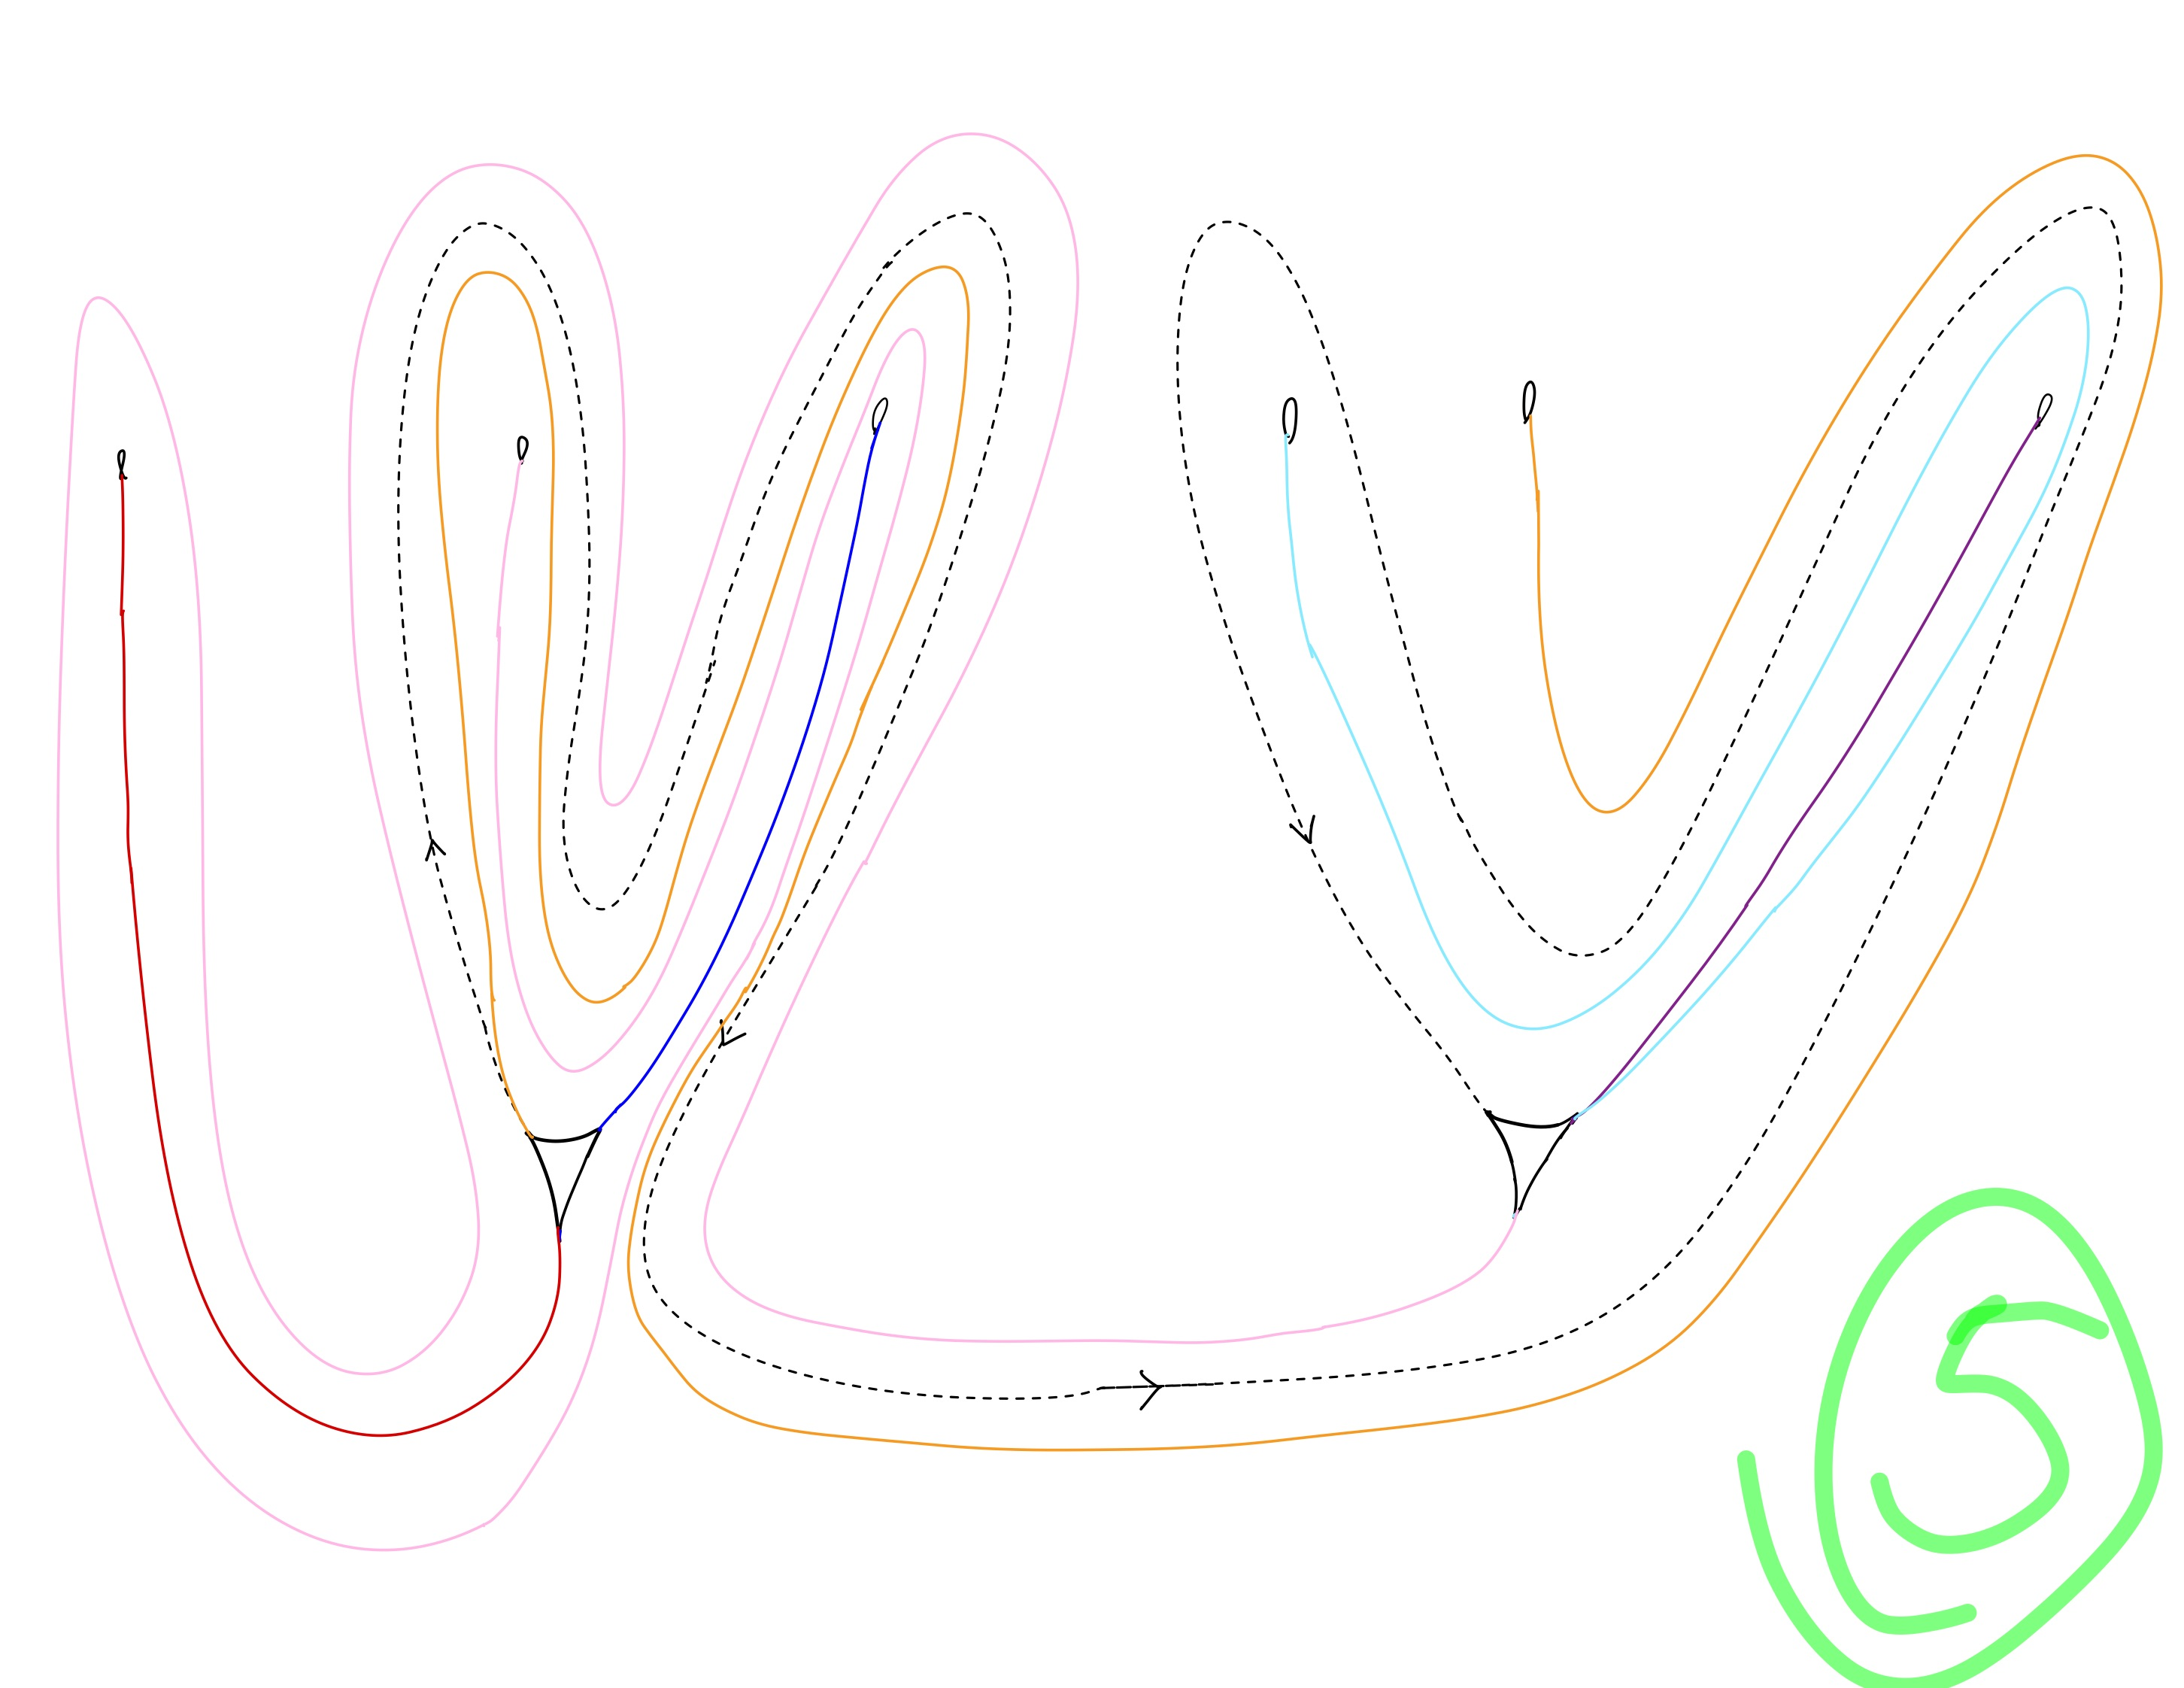
\includegraphics[width=\linewidth, height=0.45\textheight, keepaspectratio]{figures_braid/figures_track_8/Track 8 Braid 5 Quaint-1.jpg}
    \caption{Train Track Map Candidate Family 5 (Quaint) of Track 8.}
    \label{fig:track8_braid_b8_5_map}
\end{figure*}

The inverse of the following braid carries this family of train track maps:
\[
b_5^8 = \sigma_{5}^{-1} \sigma_{4}^{-1} \sigma_{1}^{-1} \sigma_{2}^{-1} \sigma_{1}^{-1} \sigma_{1}^{-1} \sigma_{1}^{-1} \sigma_{2}^{-1} \sigma_{3}^{-1} \sigma_{4}^{-1} \sigma_{3}^{-1} \sigma_{3}^{-1} \sigma_{5}^{-1} \sigma_{4}^{-1} \sigma_{3}^{-1} \sigma_{2}^{-1} \sigma_{1}^{-1}
\]

This is shown in Figure \ref{fig:track8_braid_b8_5}.

\begin{figure*}[p]
    \centering
    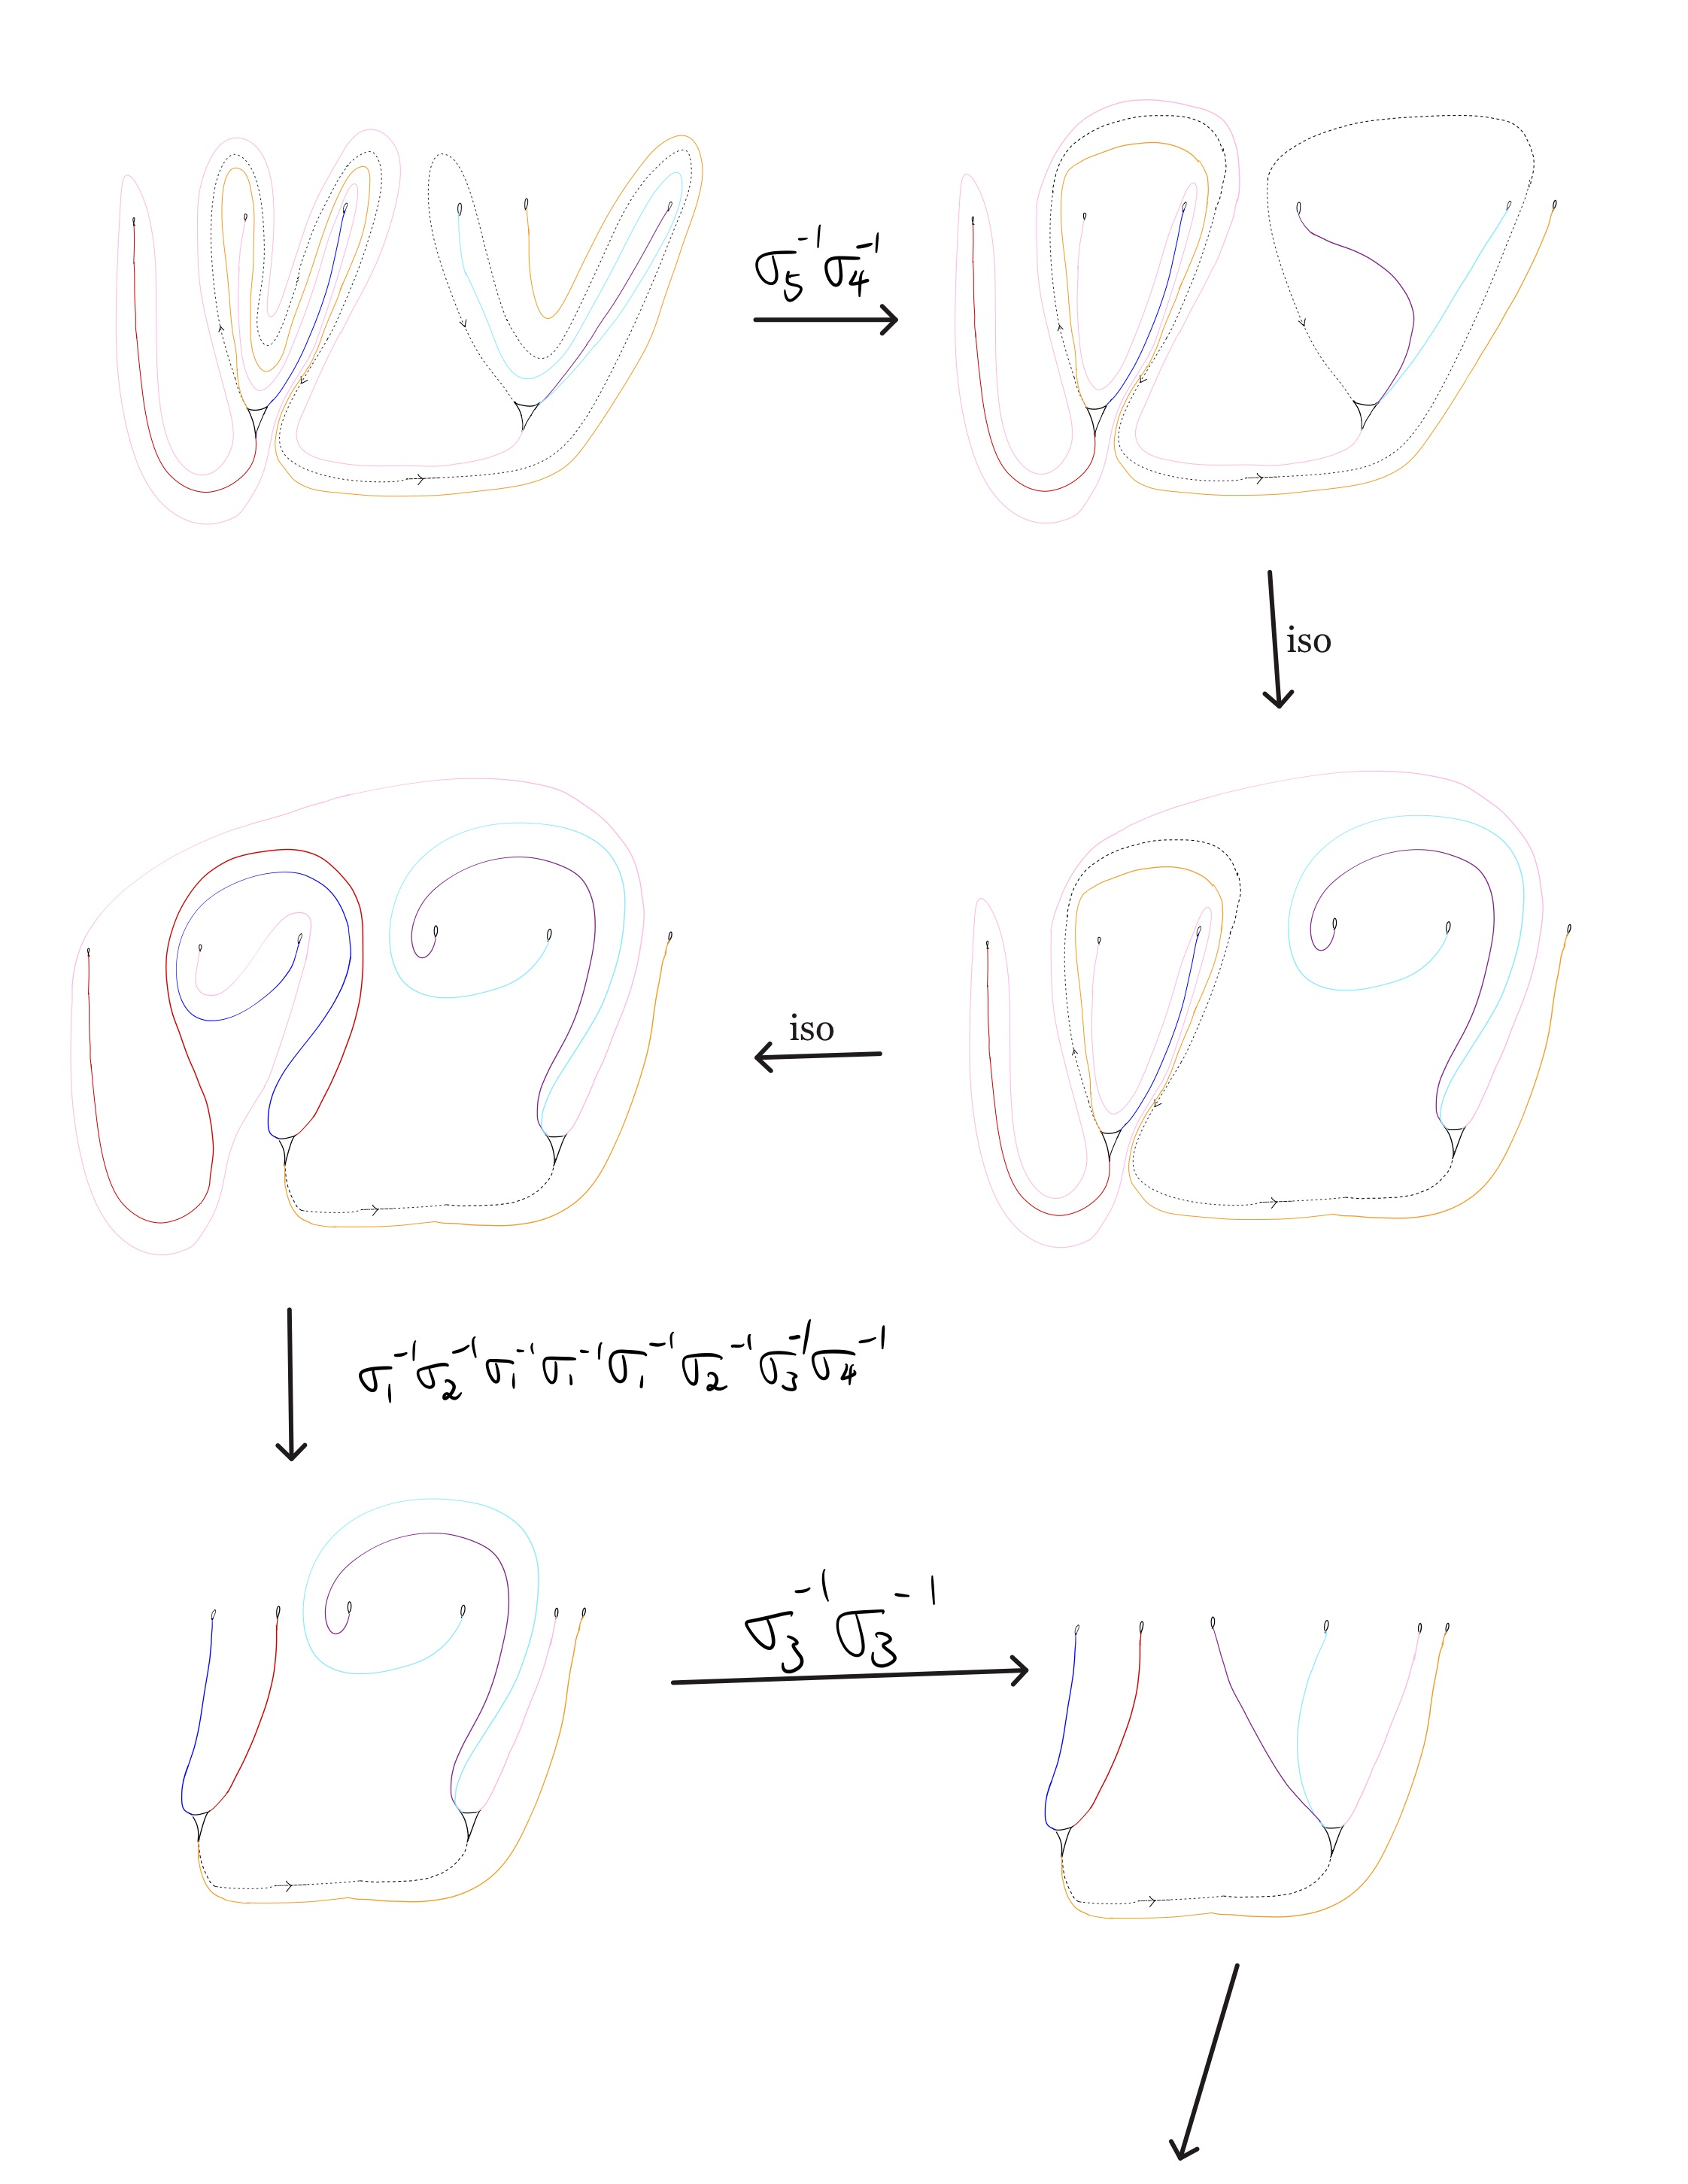
\includegraphics[width=\linewidth, height=0.45\textheight, keepaspectratio]{figures_braid/figures_track_8/Track 8 Braid 5 Quaint-2.jpg}%
    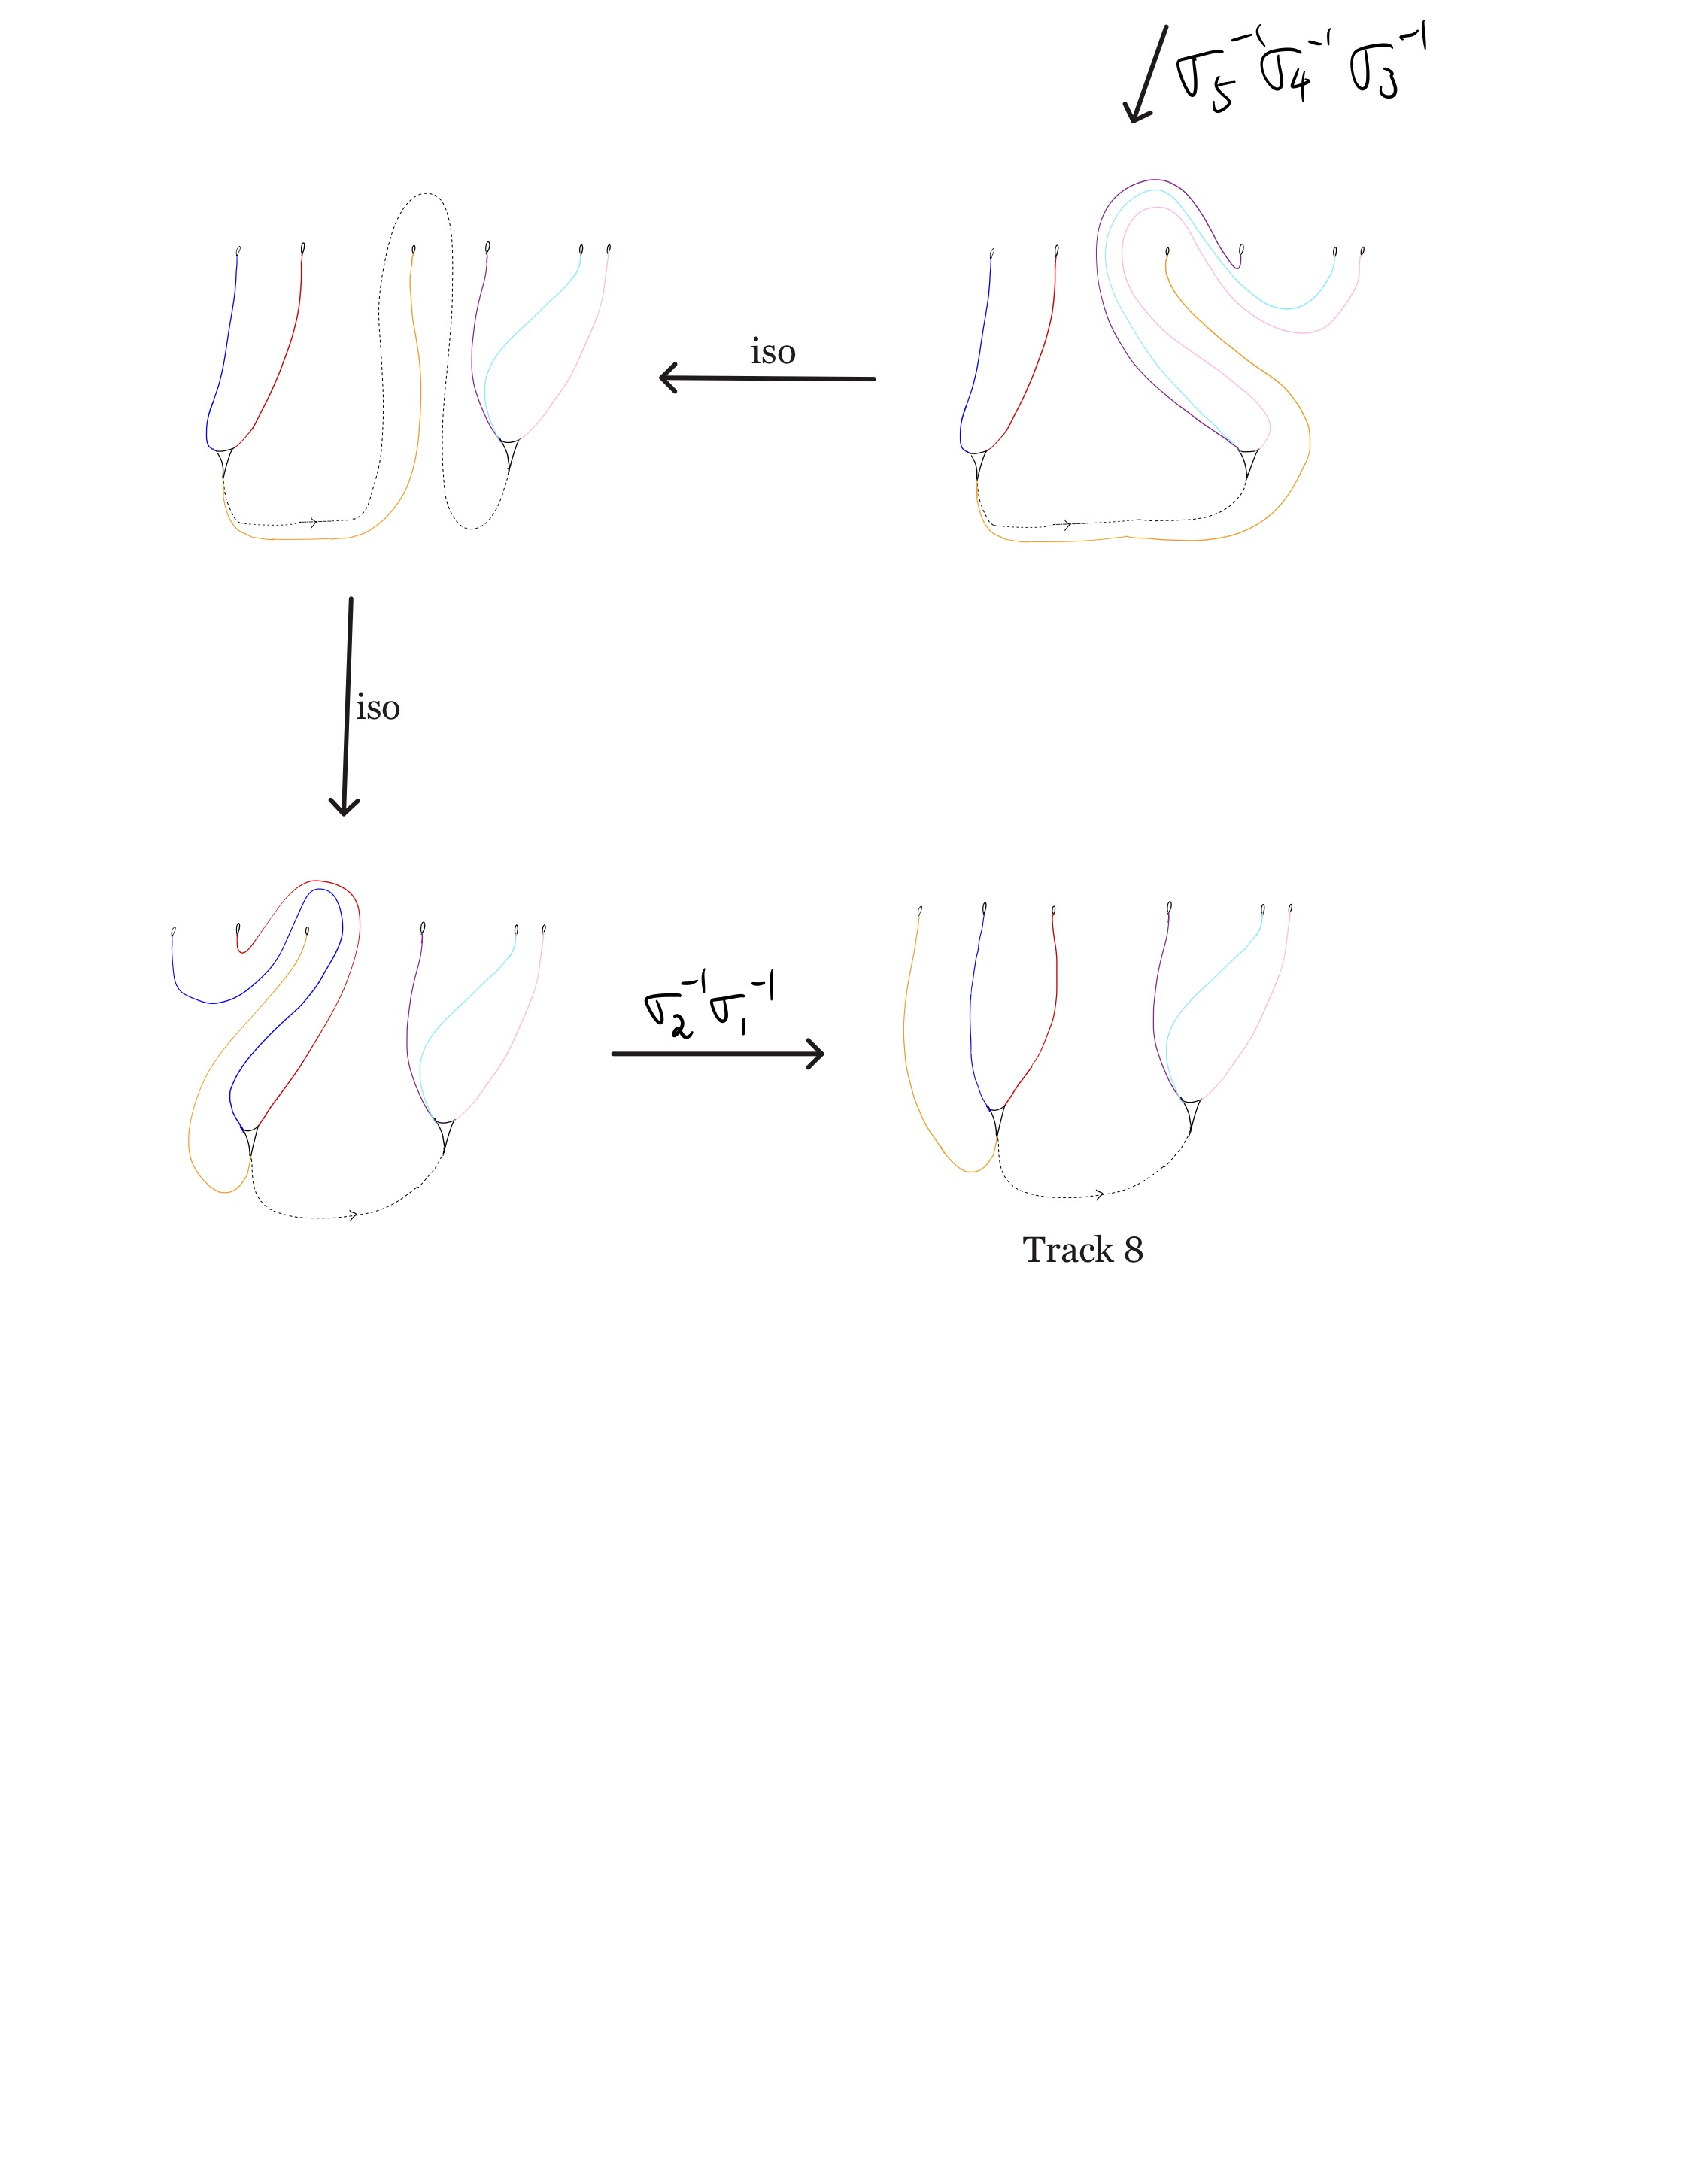
\includegraphics[width=\linewidth, height=0.45\textheight, keepaspectratio]{figures_braid/figures_track_8/Track 8 Braid 5 Quaint-3.jpg}
    \caption{This sequence shows the inverse of the braid $b_5^8$ carries Train Track Candidate Family 5.}
    \label{fig:track8_braid_b8_5}
\end{figure*}

\clearpage

\section{Candidate Family 6 (Lacuna)}\label{sec:track8_lacuna}
Train Track Map Candidate Family 6 of Track 8 is shown in Figure \ref{fig:track8_braid_b8_6_map}. See \ref{Lacuna} for details.

\begin{figure*}[ht]
    \centering
    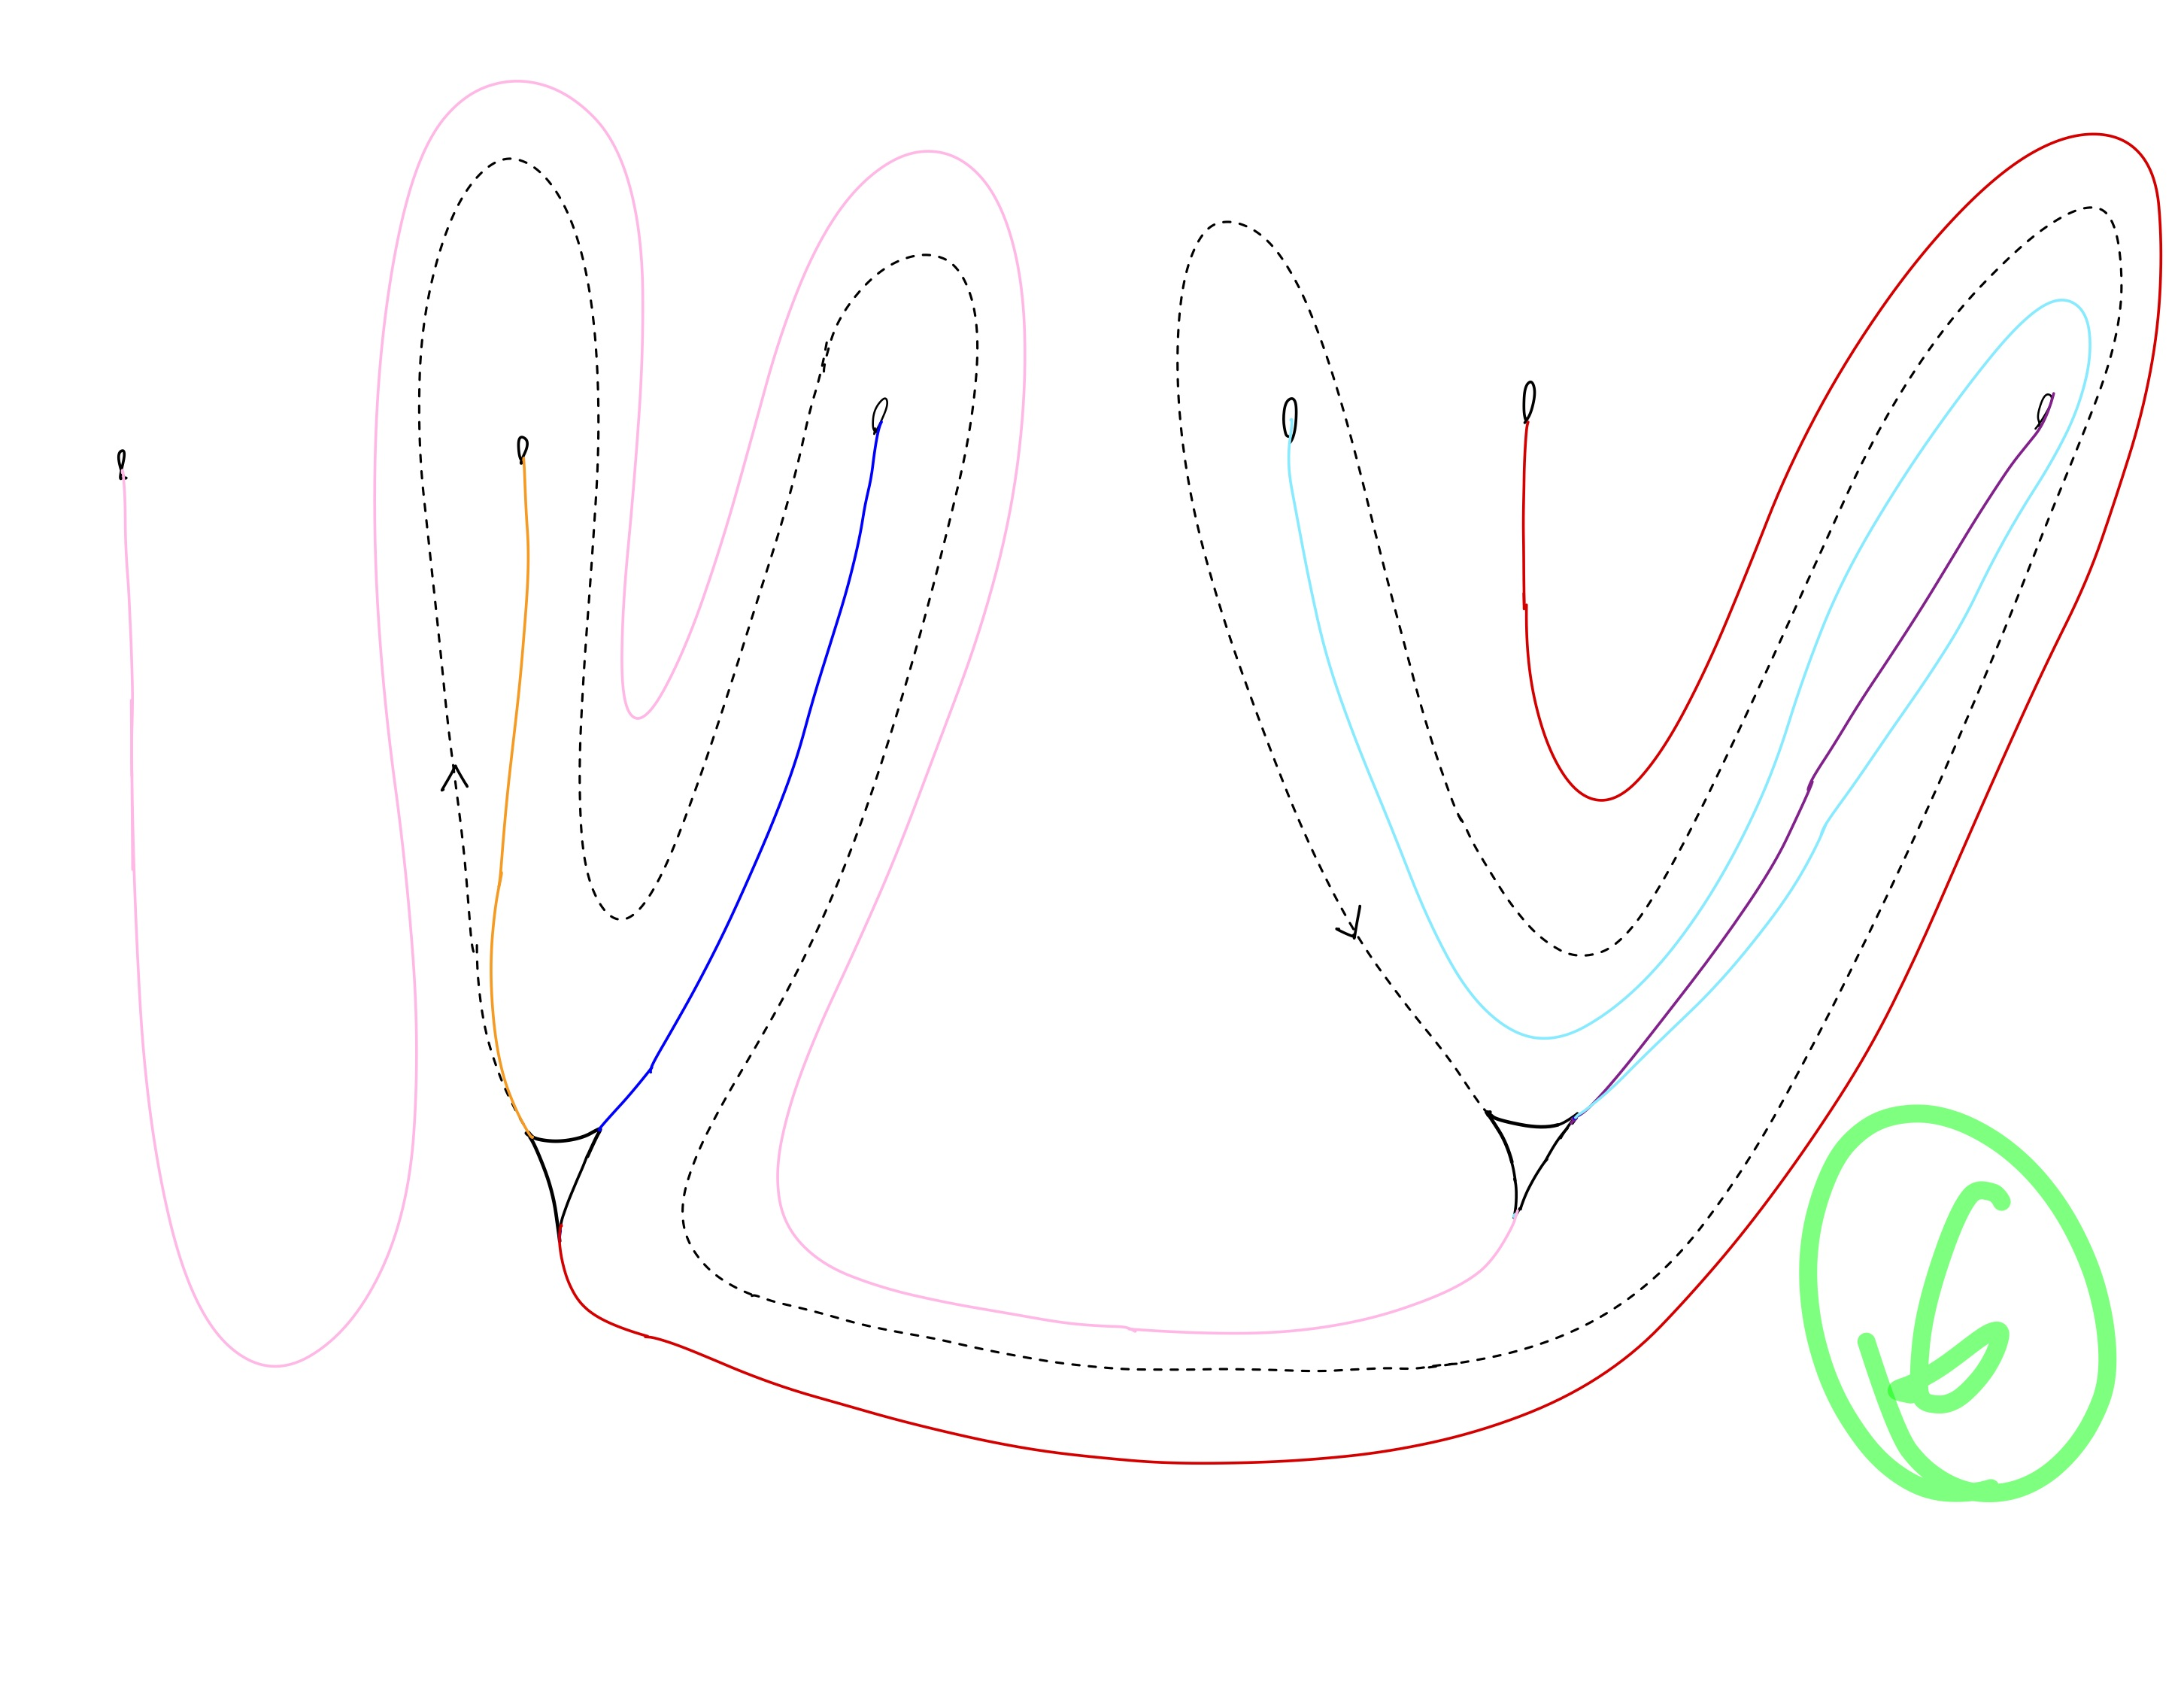
\includegraphics[width=\linewidth, height=0.45\textheight, keepaspectratio]{figures_braid/figures_track_8/Track 8 Braid 6 Lacuna-1.jpg}
    \caption{Train Track Map Candidate Family 6 (Lacuna) of Track 8.}
    \label{fig:track8_braid_b8_6_map}
\end{figure*}

The inverse of the following braid carries this family of train track maps:
\[
b_6^8 = \sigma_{5}^{-1} \sigma_{1}^{-1} \sigma_{2}^{-1} \sigma_{4}^{-1} \sigma_{3}^{-1} \sigma_{4}^{-1} \sigma_{5}^{-1} \sigma_{3}^{-1} \sigma_{3}^{-1} \sigma_{4}^{-1} \sigma_{3}^{-1} \sigma_{2}^{-1} \sigma_{1}^{-1} \sigma_{1}^{-1} \sigma_{2}^{-1} \sigma_{1}^{-1} \sigma_{1}^{-1}
\]

This is shown in Figure \ref{fig:track8_braid_b8_6}.

\begin{figure*}[p]
    \centering
    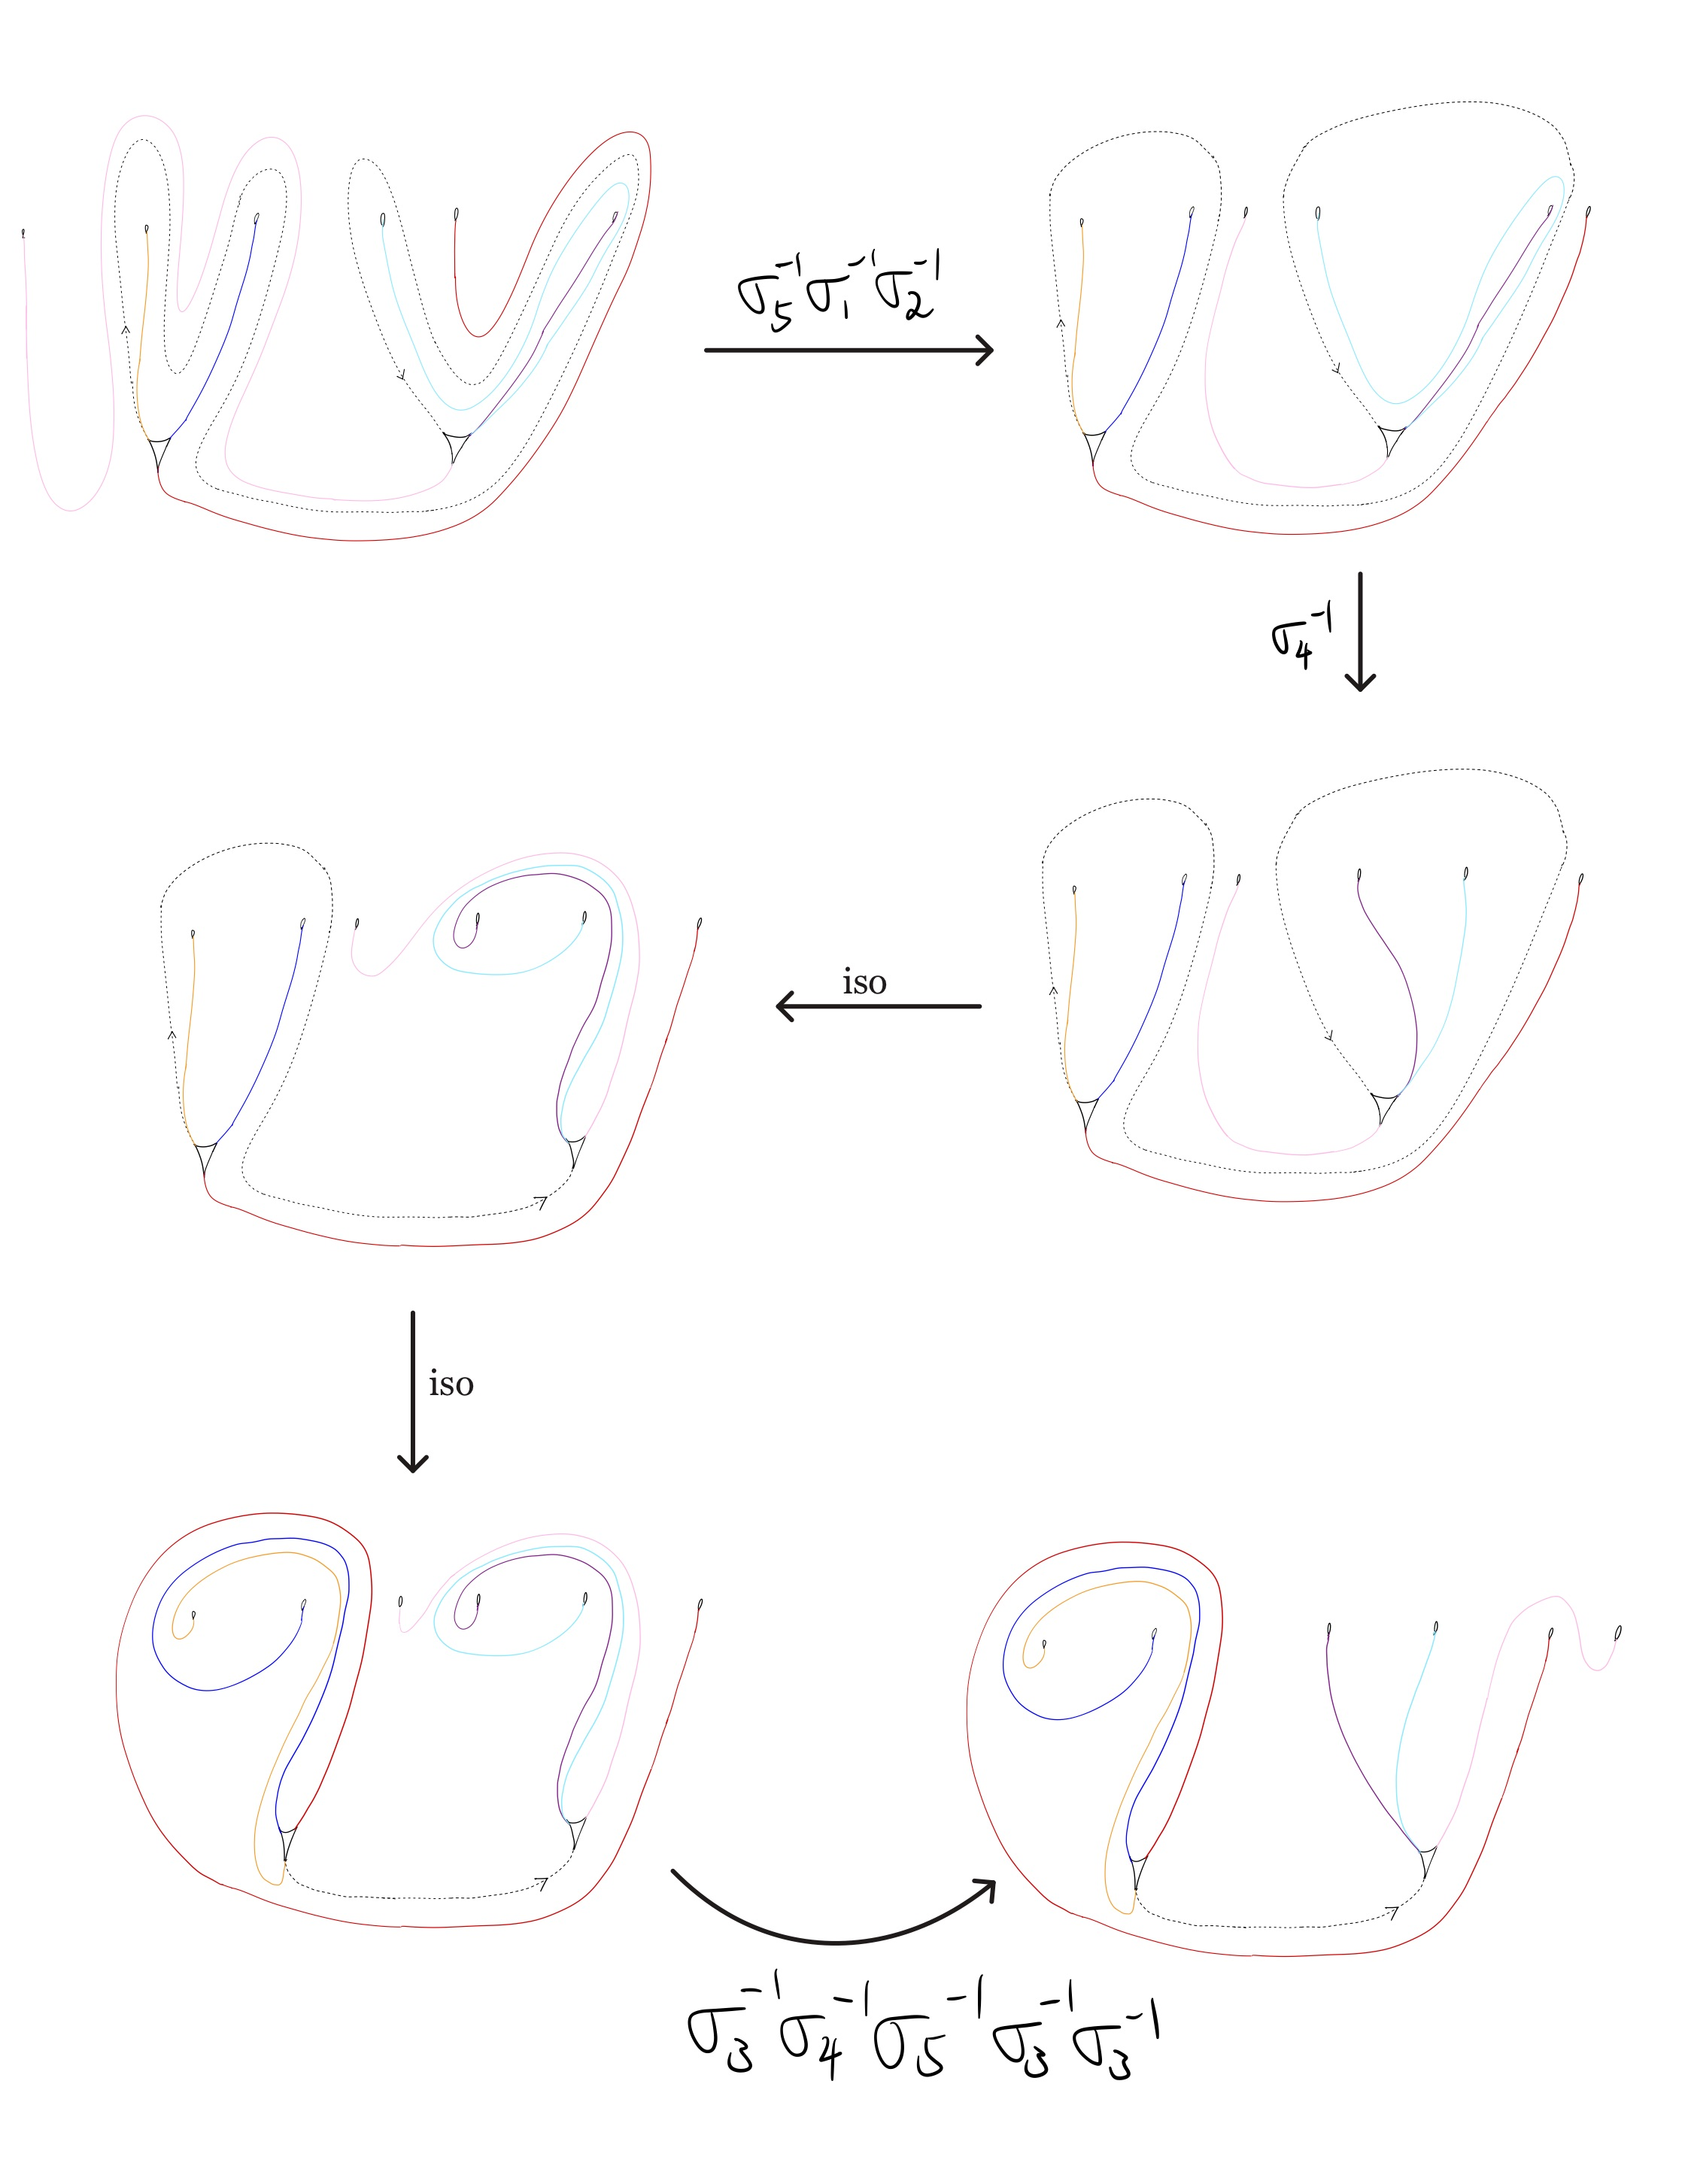
\includegraphics[width=\linewidth, height=0.45\textheight, keepaspectratio]{figures_braid/figures_track_8/Track 8 Braid 6 Lacuna-2.jpg}%
    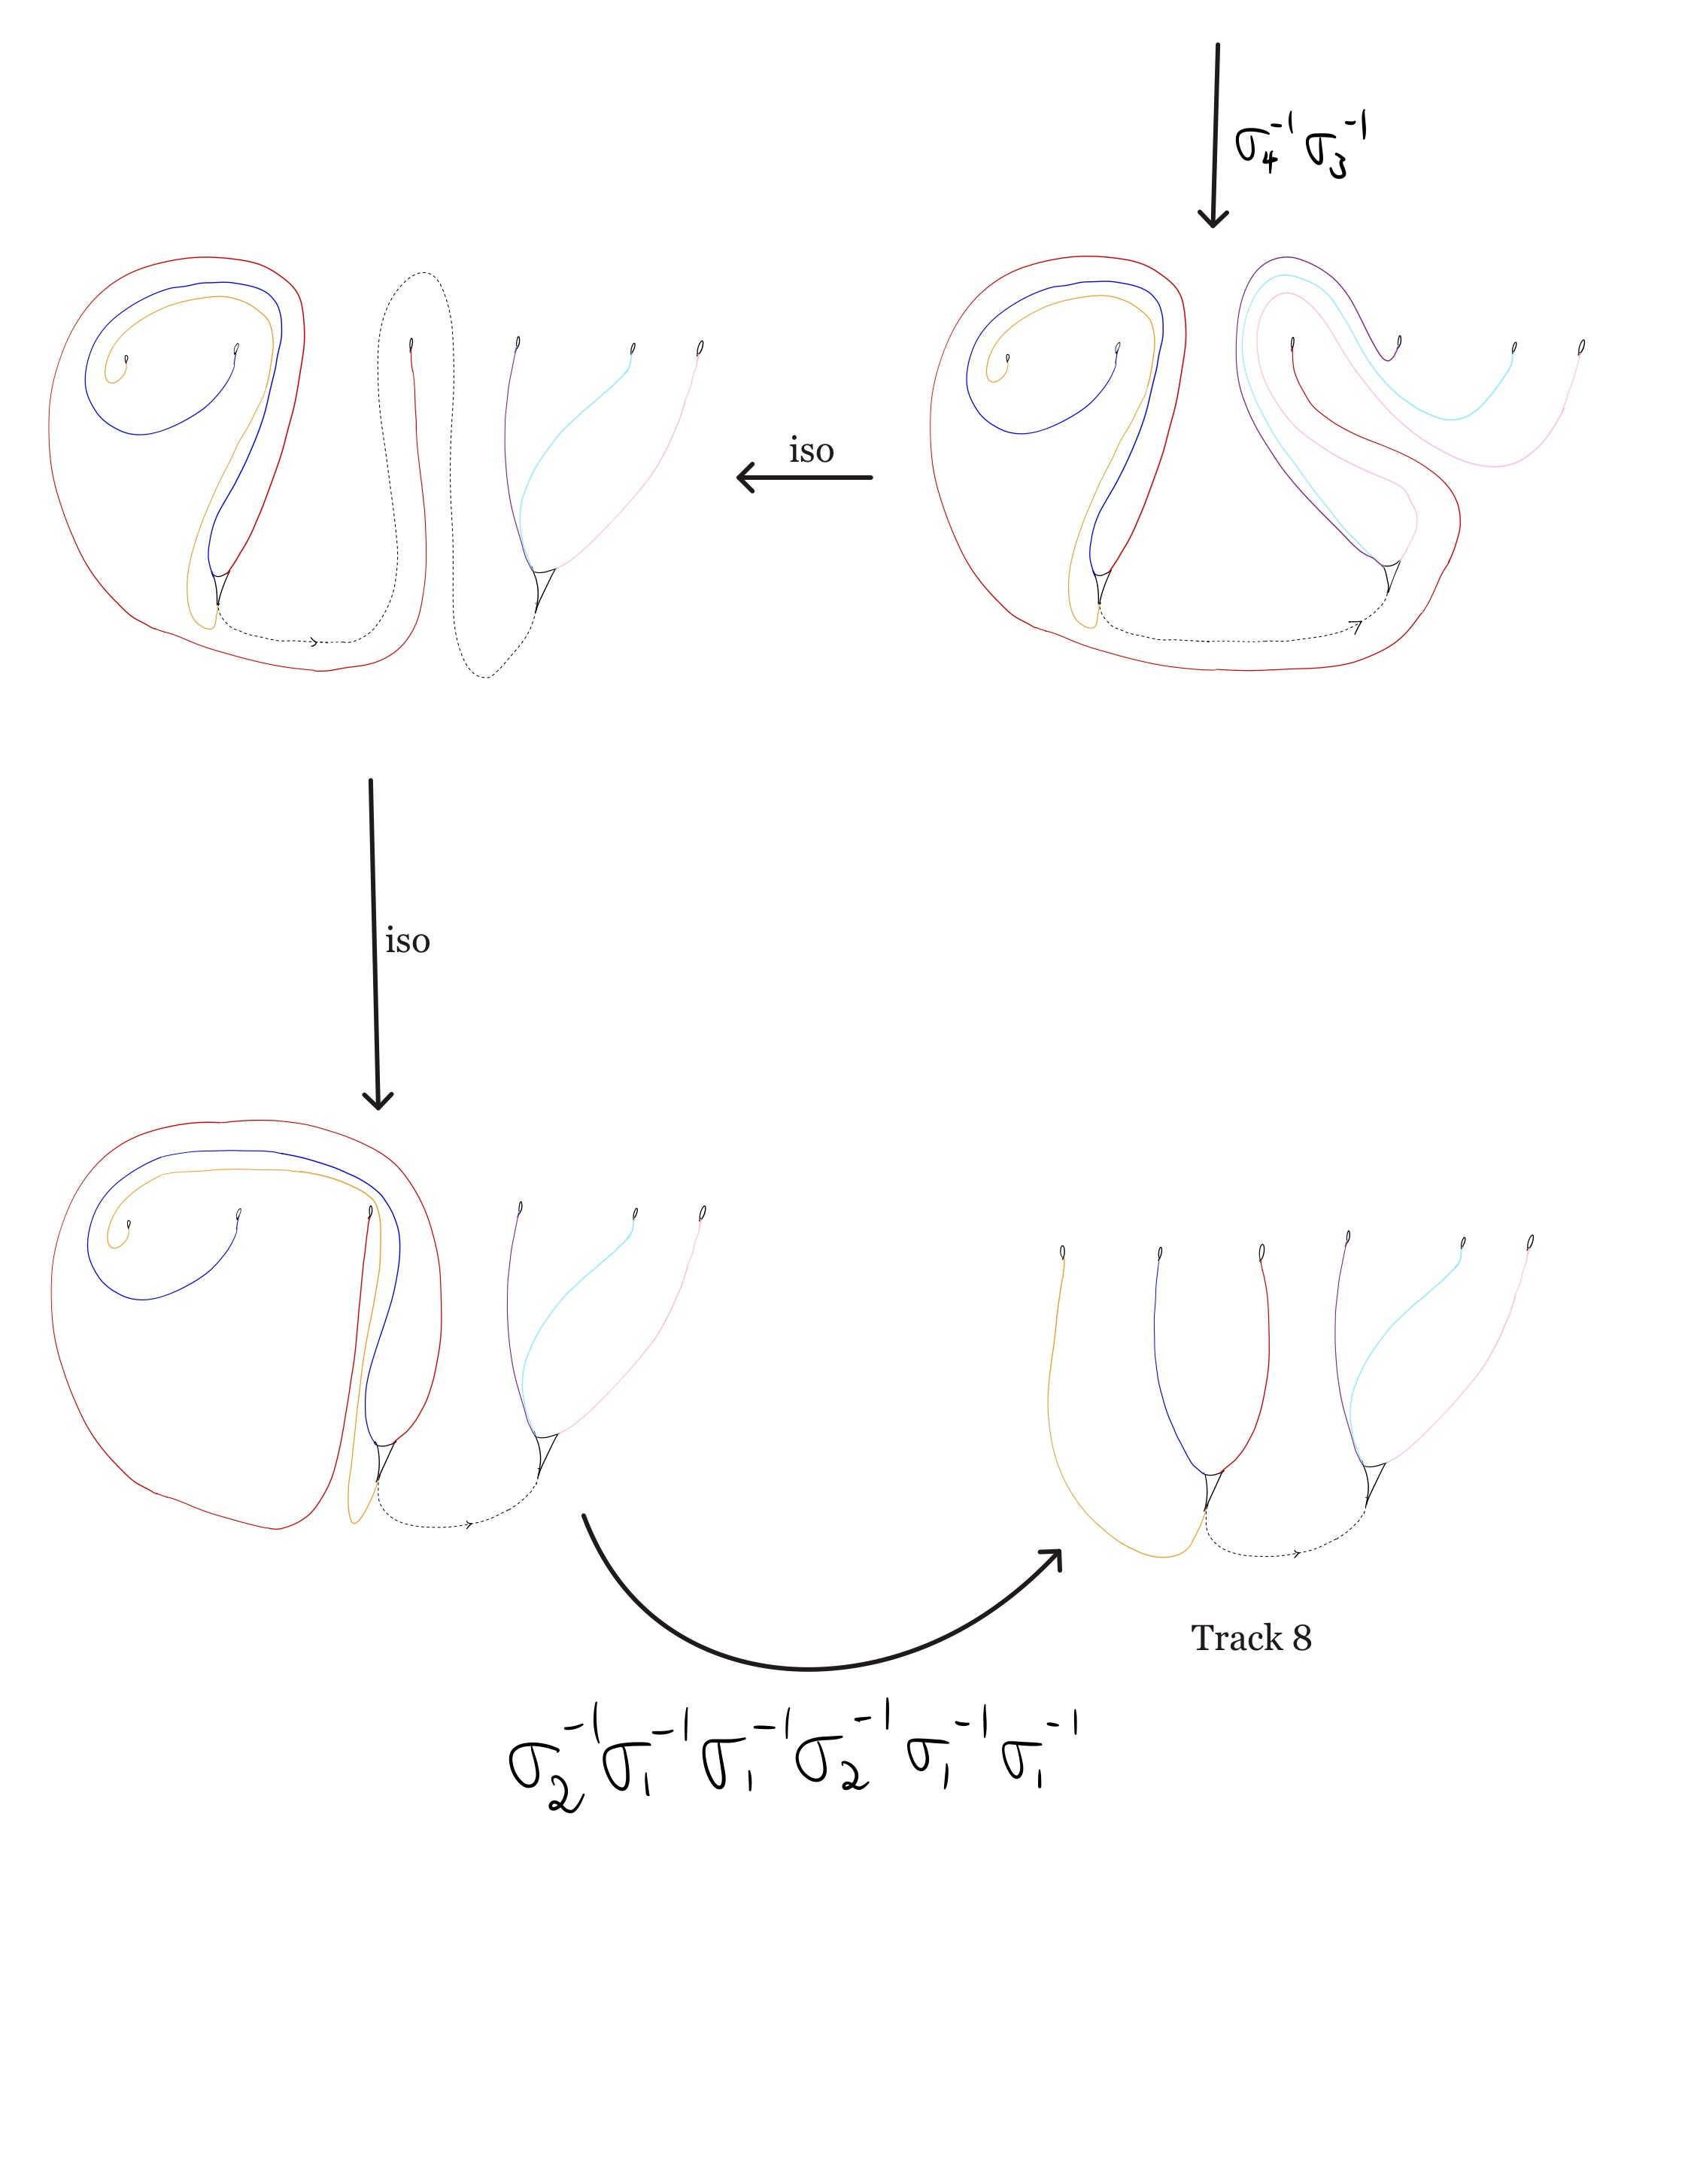
\includegraphics[width=\linewidth, height=0.45\textheight, keepaspectratio]{figures_braid/figures_track_8/Track 8 Braid 6 Lacuna-3.jpg}
    \caption{This sequence shows the inverse of the braid $b_6^8$ carries Train Track Candidate Family 6.}
    \label{fig:track8_braid_b8_6}
\end{figure*}

\clearpage

\section{Candidate Family 7 (Aulic)}\label{sec:track8_aulic}
Train Track Map Candidate Family 7 of Track 8 is shown in Figure \ref{fig:track8_braid_b8_7_map}. See \ref{Aulic} for details.

\begin{figure*}[ht]
    \centering
    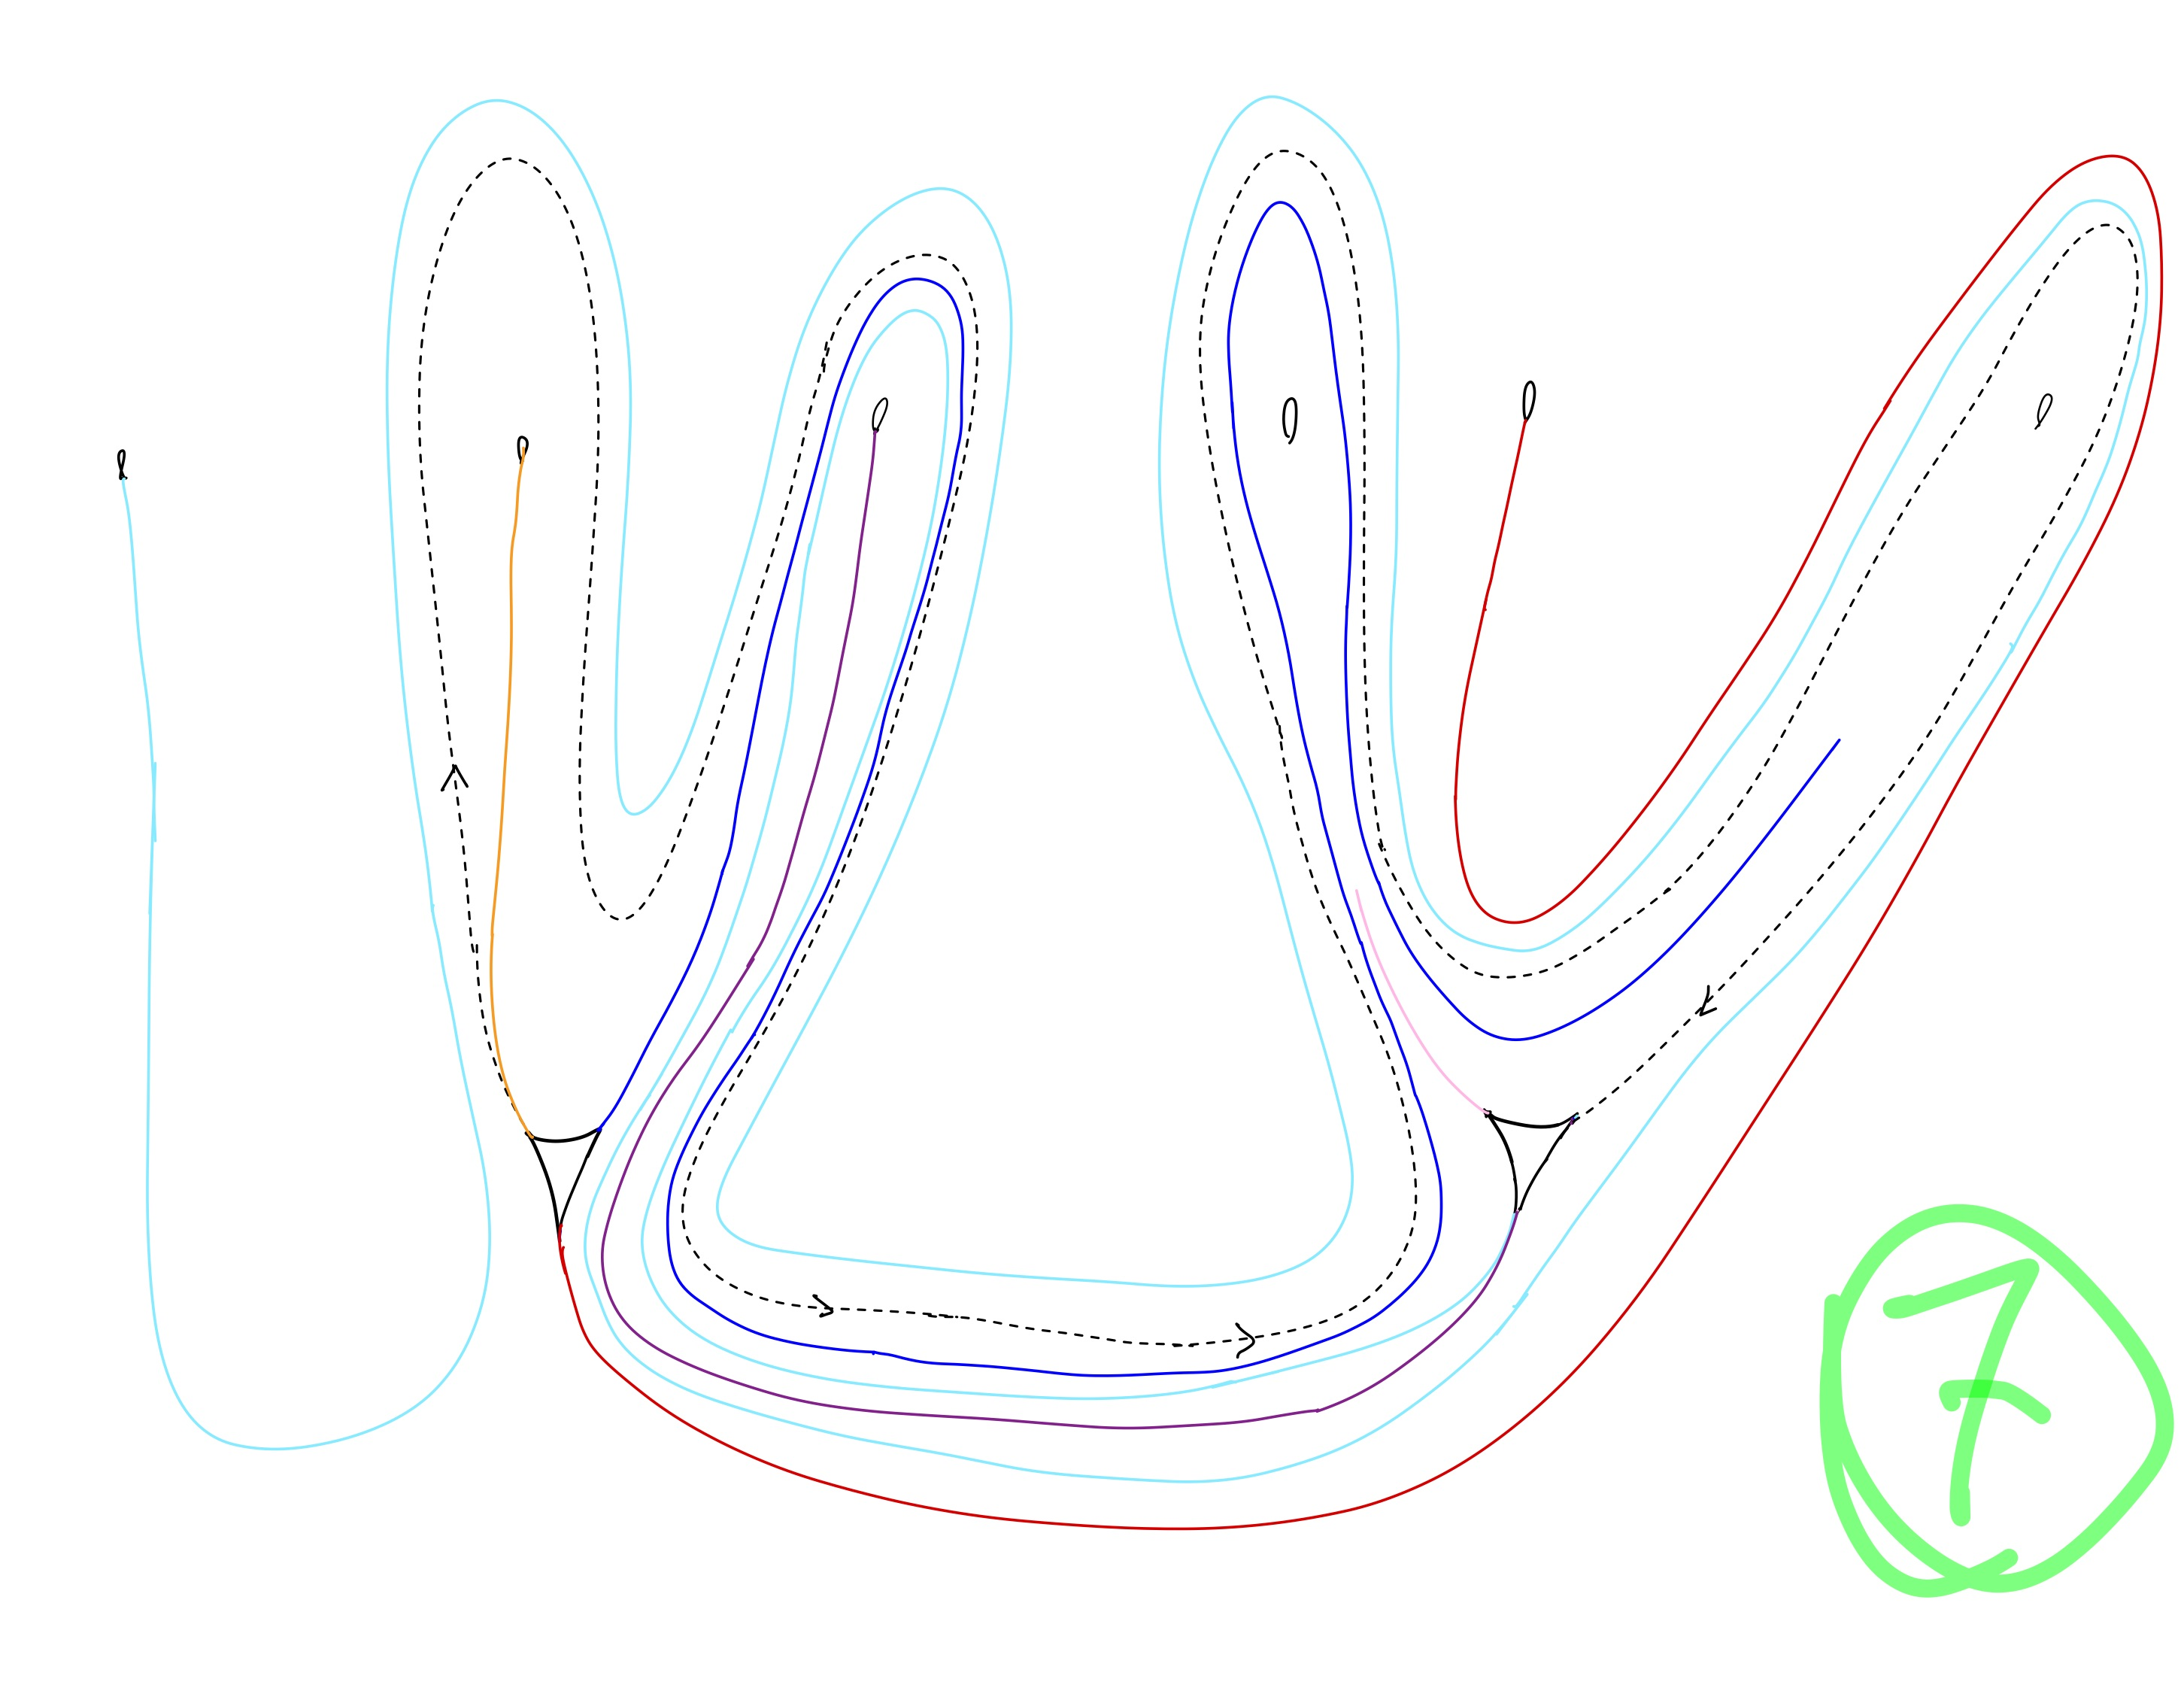
\includegraphics[width=\linewidth, height=0.45\textheight, keepaspectratio]{figures_braid/figures_track_8/Track 8 Braid 7 Aulic-1.jpg}
    \caption{Train Track Map Candidate Family 7 (Aulic) of Track 8.}
    \label{fig:track8_braid_b8_7_map}
\end{figure*}

The inverse of the following braid carries this family of train track maps:
\[
b_7^8 = \sigma_{5}^{-1} \sigma_{4}^k \sigma_{3} \sigma_{1}^{-1} \sigma_{2}^{-1} \sigma_{3}^{-1} \sigma_{4}^{-1} \sigma_{3} \sigma_{3} \sigma_{2} \sigma_{1} \sigma_{4} \sigma_{3} \sigma_{2} \sigma_{4} \sigma_{3} \circ \Lambda_6 \circ J
\]
where $k \geq 1$ ($k \in \mathbb{Z}$) is the twisting parameter. This is shown in Figure \ref{fig:track8_braid_b8_7}.

\begin{figure*}[p]
    \centering
    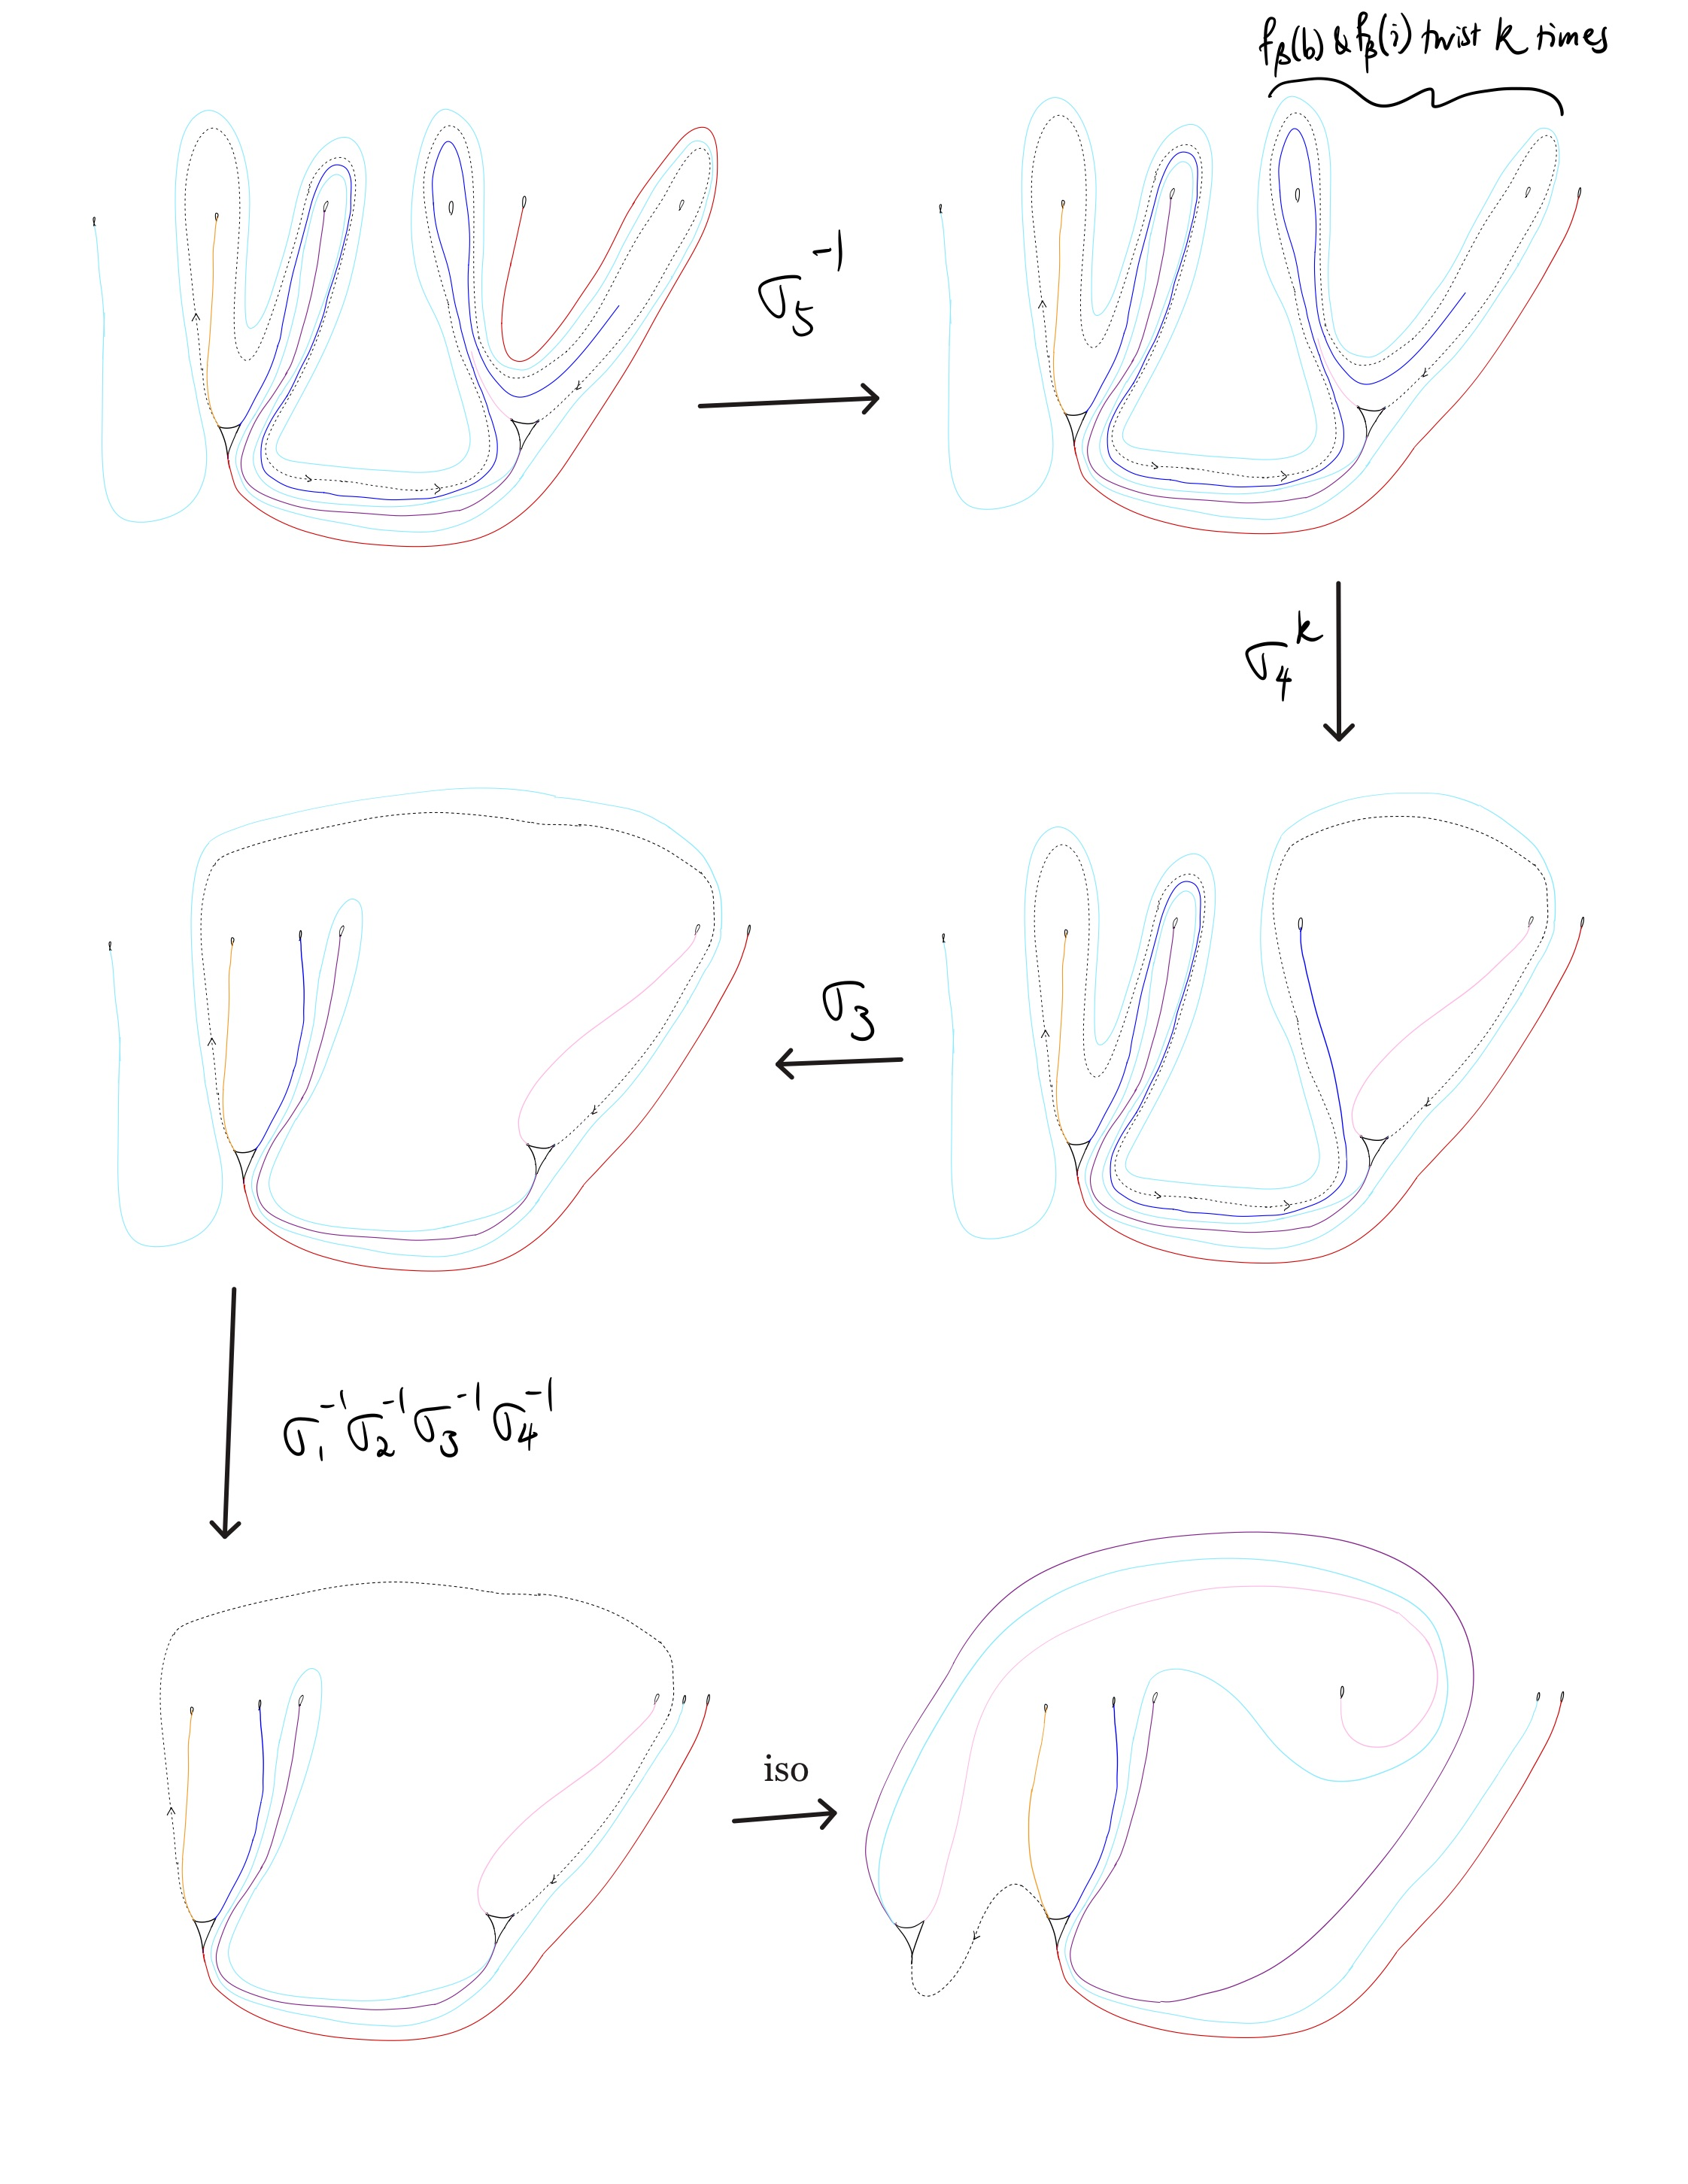
\includegraphics[width=\linewidth, height=0.45\textheight, keepaspectratio]{figures_braid/figures_track_8/Track 8 Braid 7 Aulic-2.jpg}%
    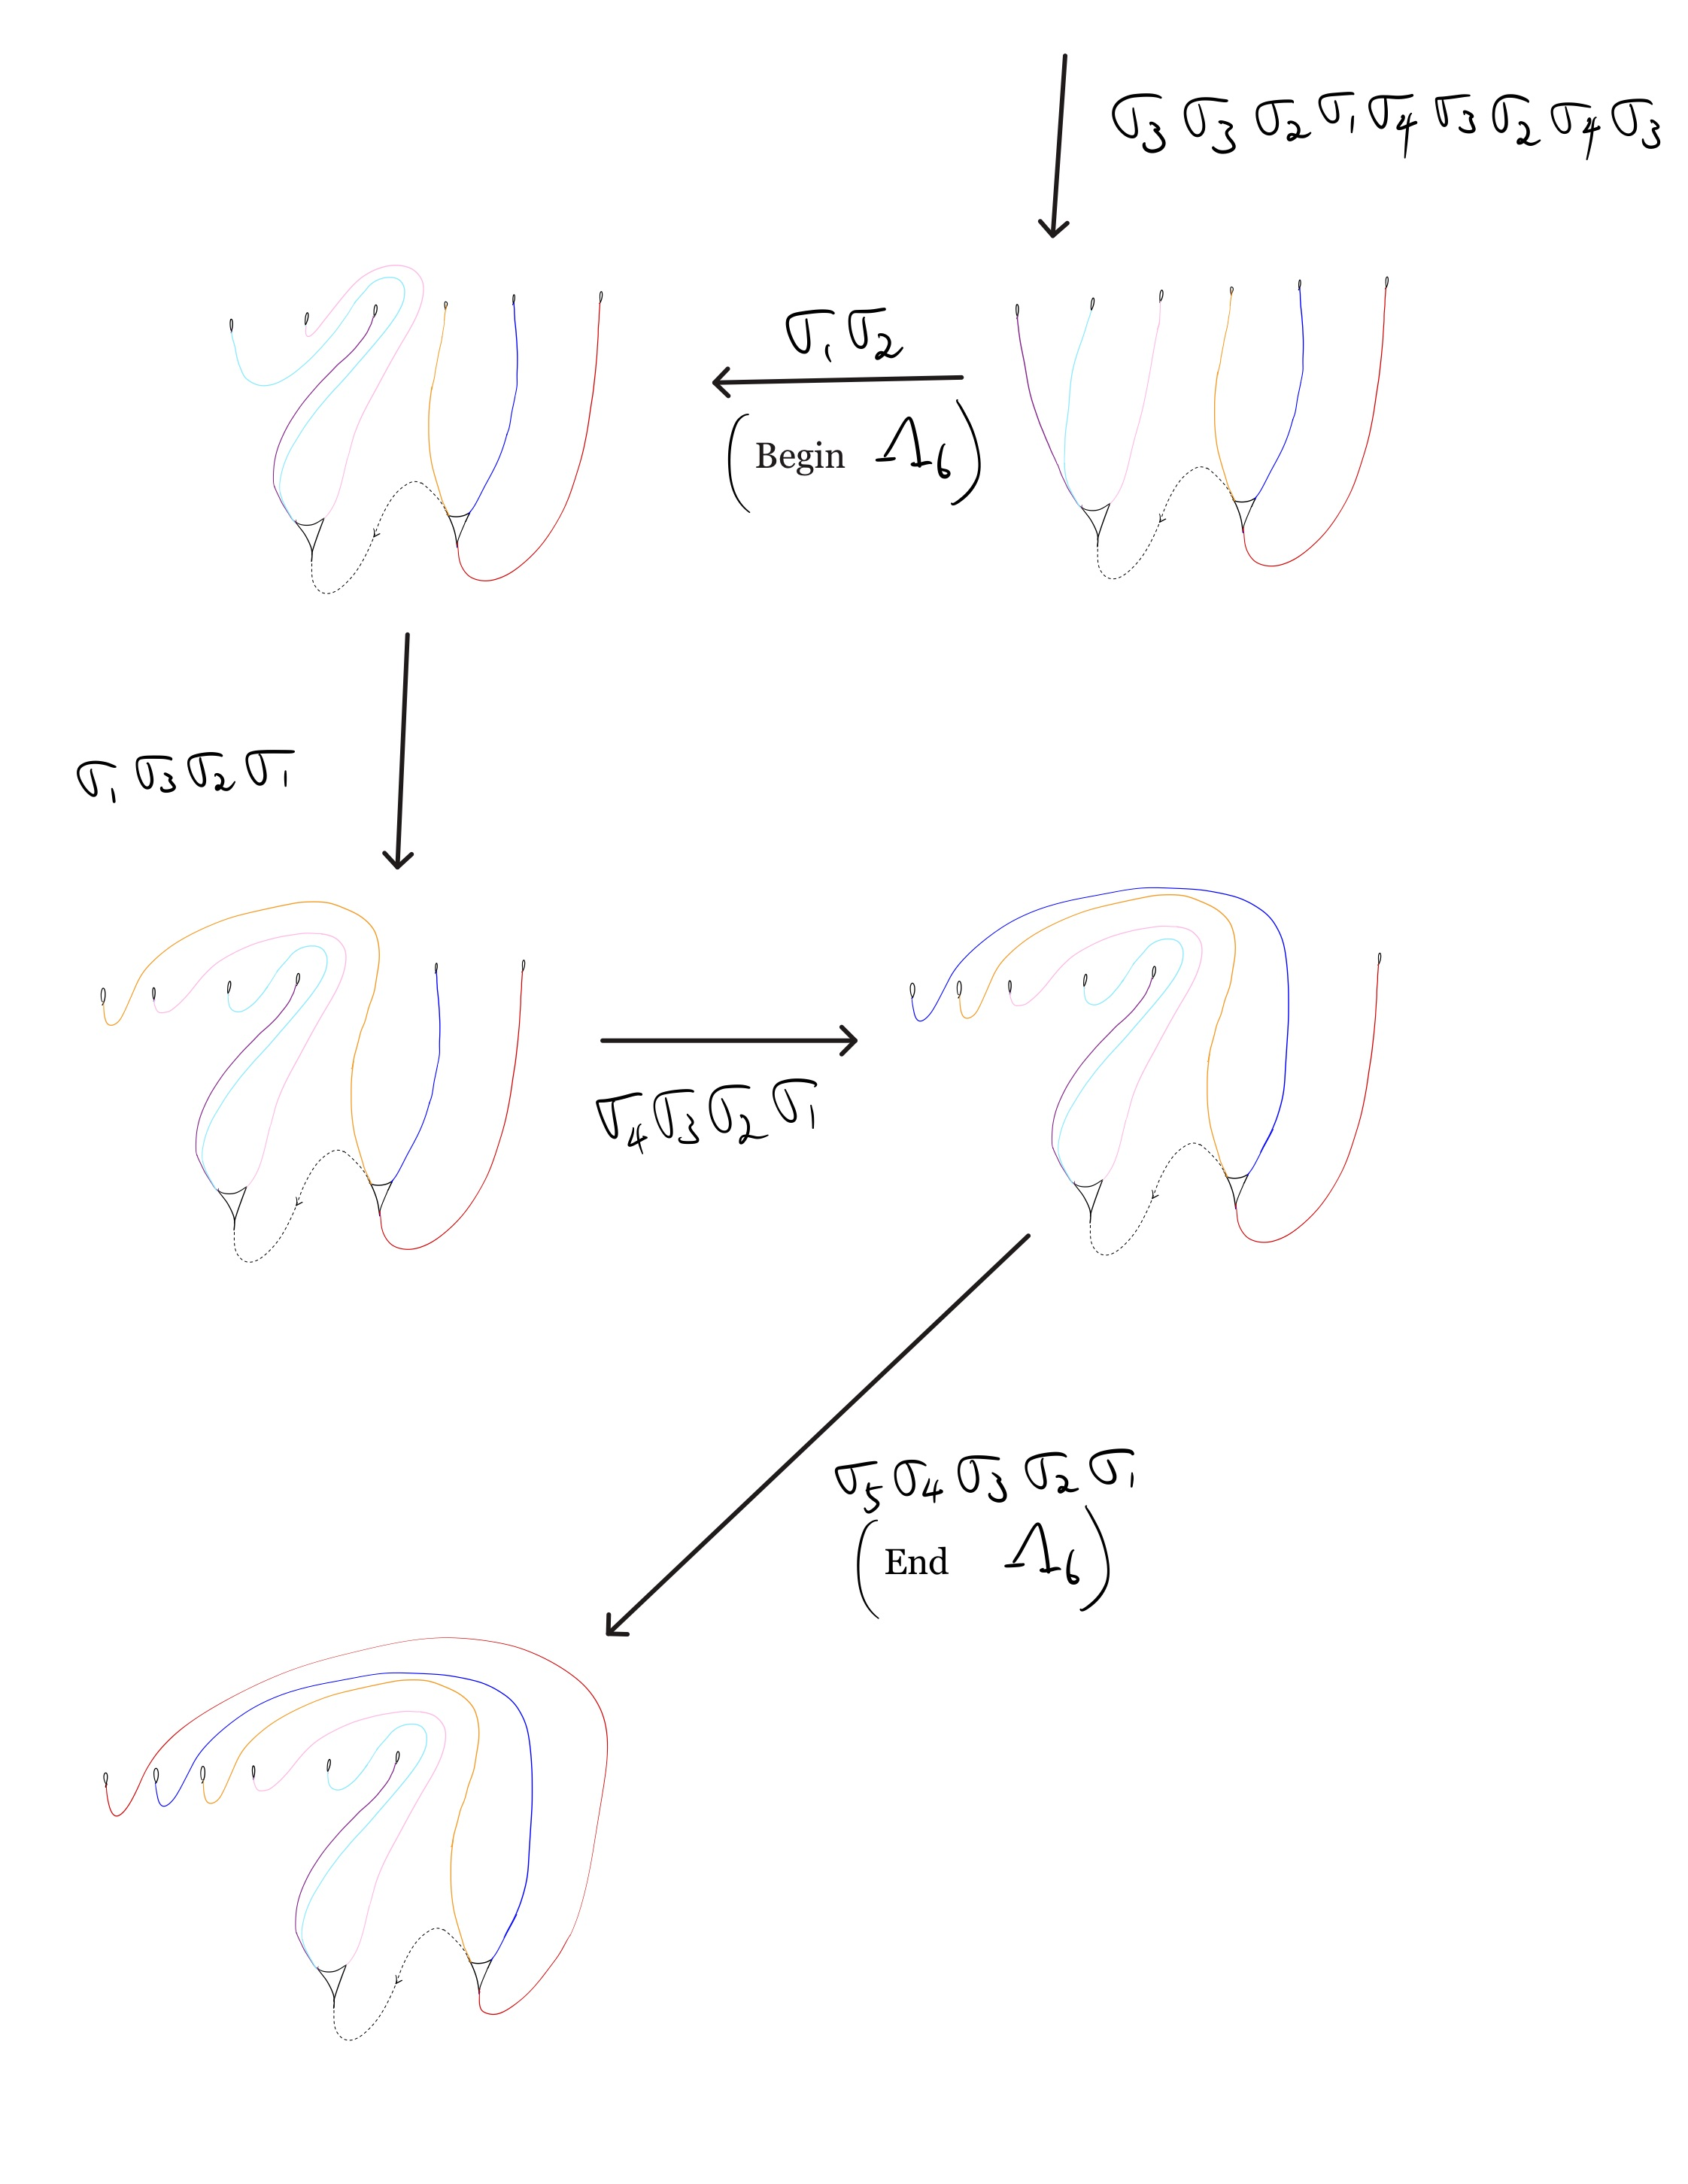
\includegraphics[width=\linewidth, height=0.45\textheight, keepaspectratio]{figures_braid/figures_track_8/Track 8 Braid 7 Aulic-3.jpg}
    \caption{This sequence shows the inverse of the braid $b_7^8$ carries Train Track Candidate Family 7.}
    \label{fig:track8_braid_b8_7}
\end{figure*}

\clearpage

\section{Candidate Family 8 (Oread)}\label{sec:track8_oread}
Train Track Map Candidate Family 8 of Track 8 is shown in Figure \ref{fig:track8_braid_b8_8_map}. See \ref{Oread} for details.

\begin{figure*}[ht]
    \centering
    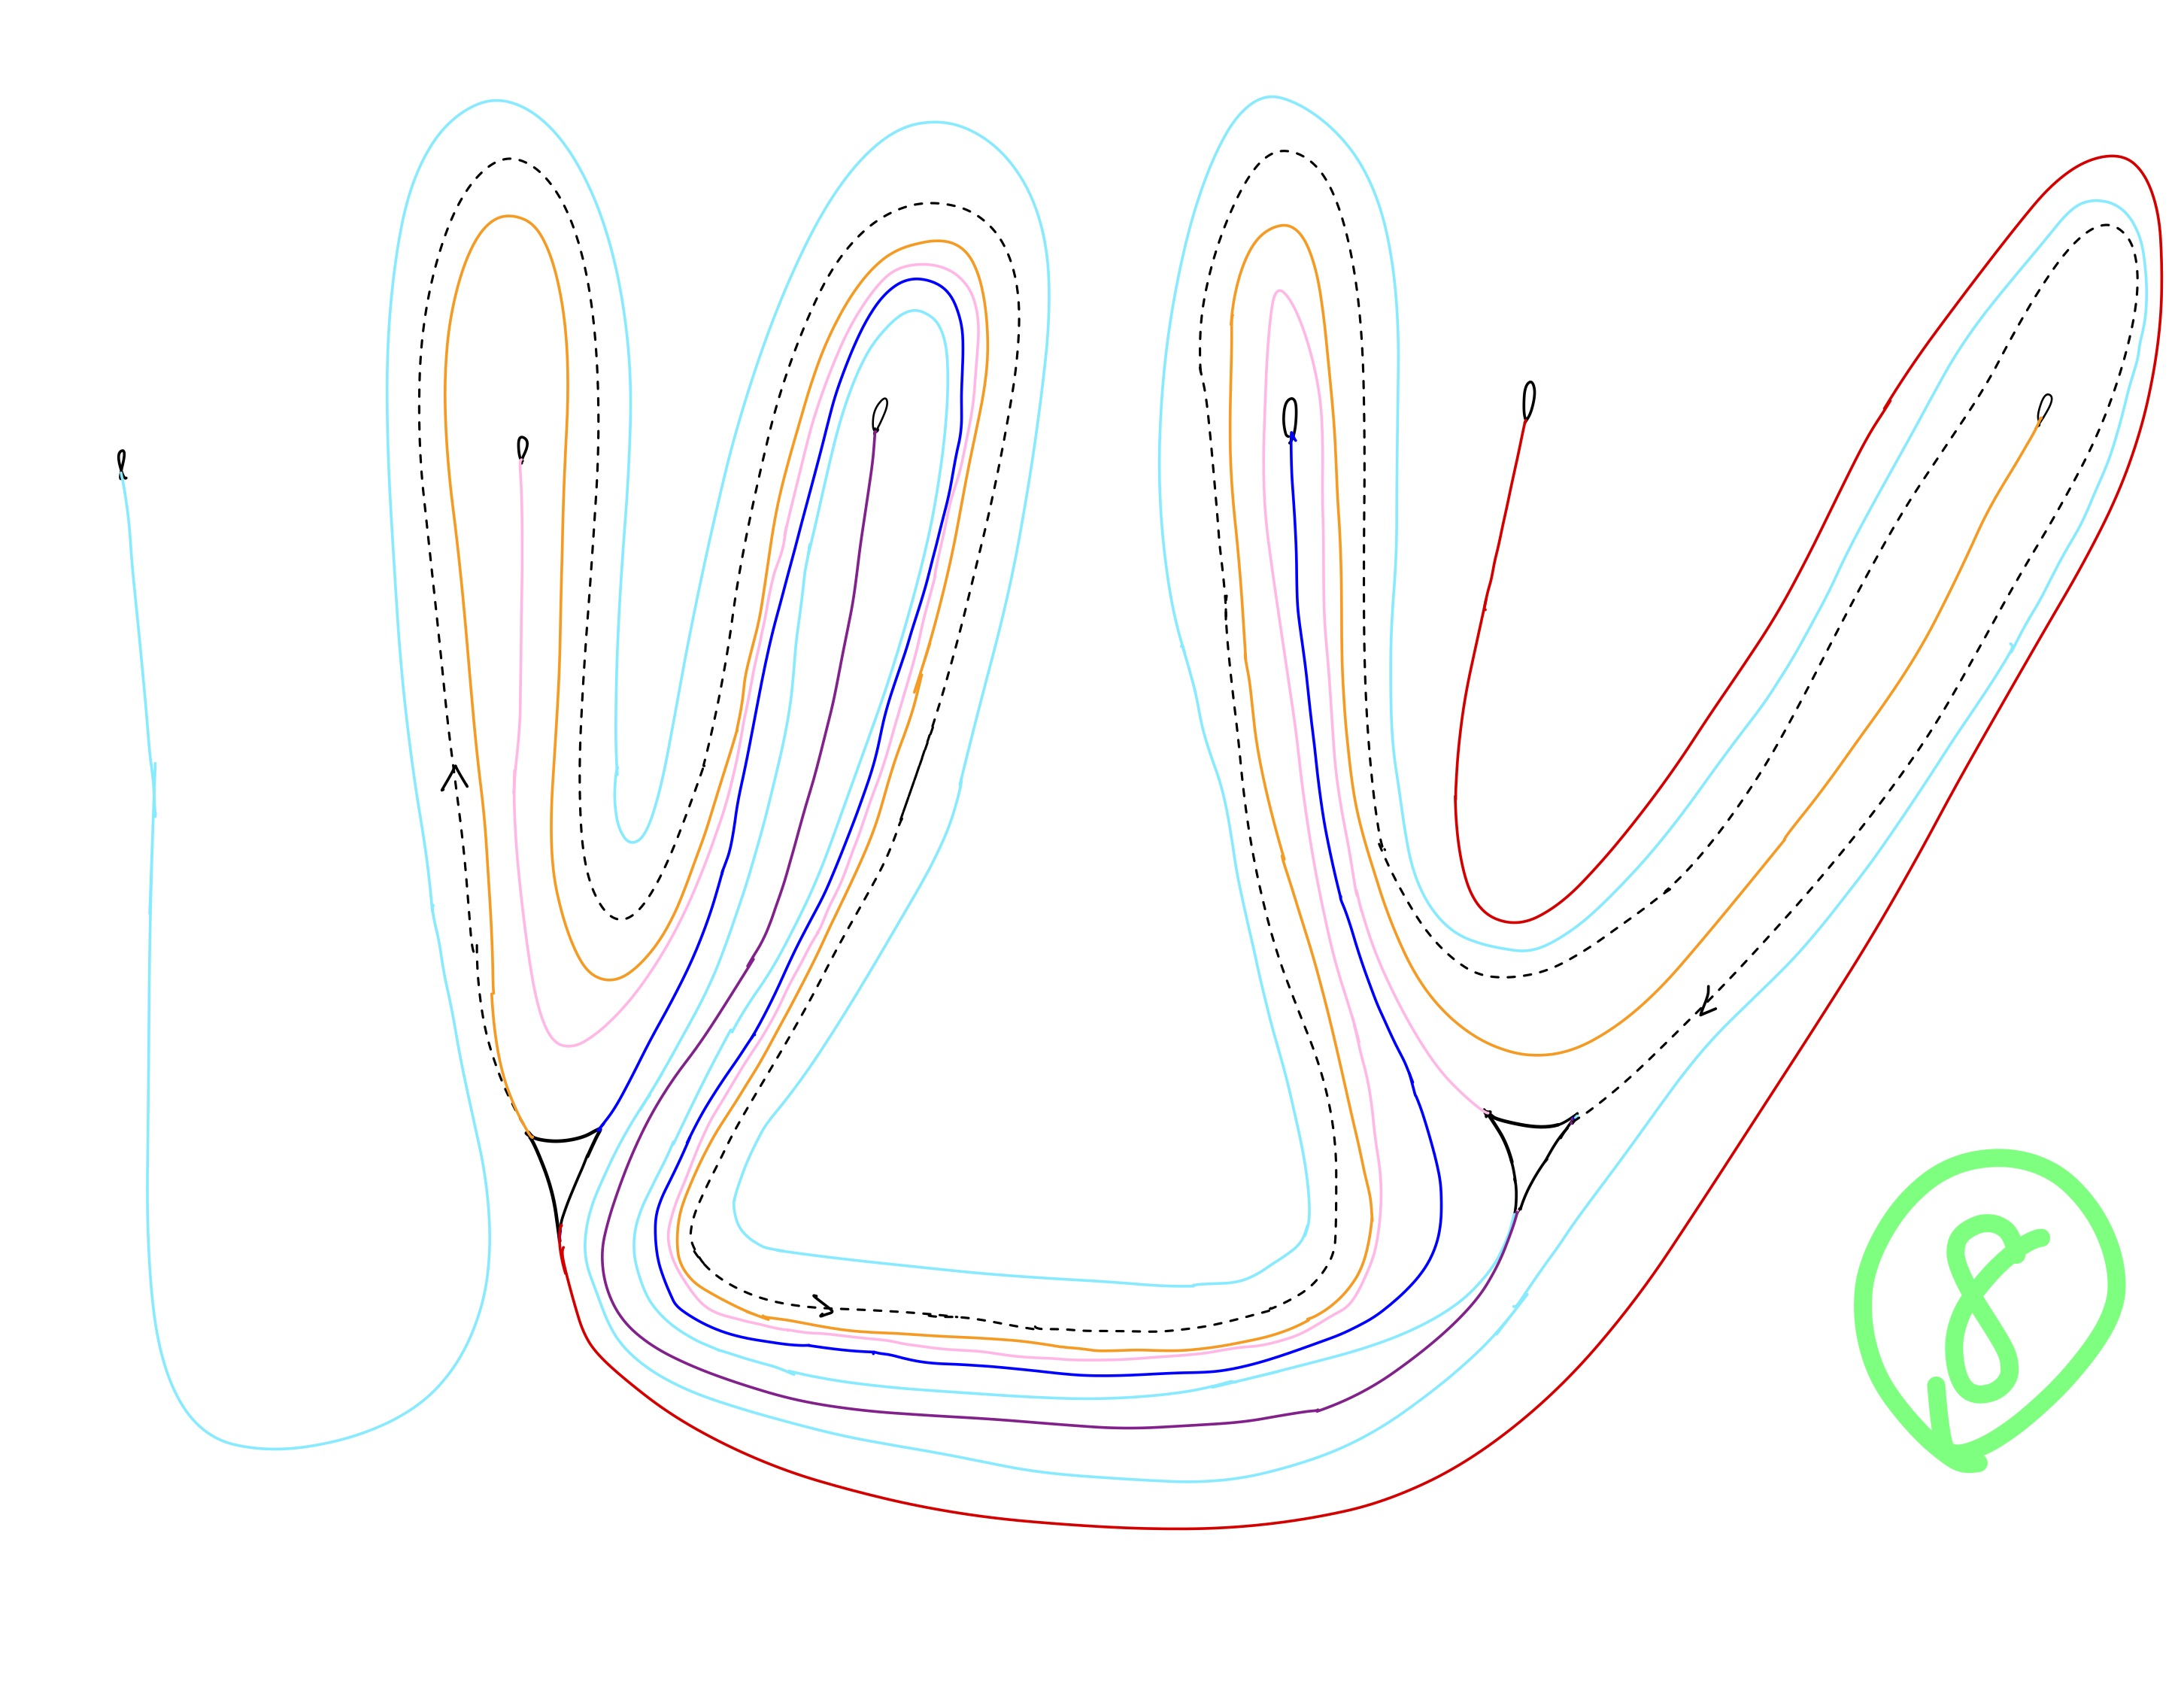
\includegraphics[width=\linewidth, height=0.45\textheight, keepaspectratio]{figures_braid/figures_track_8/Track 8 Braid 8 Oread-1.jpg}
    \caption{Train Track Map Candidate Family 8 (Oread) of Track 8.}
    \label{fig:track8_braid_b8_8_map}
\end{figure*}

The inverse of the following braid carries this family of train track maps:
\[
b_8^8 = \sigma_{5}^{-1} \sigma_{1}^{-1} \sigma_{2}^{-1} \sigma_{3}^{-1} \sigma_{4}^{-1} \sigma_{3} \sigma_{2} \sigma_{1} \sigma_{2}^{-1} \sigma_{3}^{-1} \sigma_{2} \sigma_{3} \sigma_{3} \sigma_{2} \sigma_{1} \sigma_{4} \sigma_{3} \sigma_{2} \sigma_{4} \sigma_{3} \circ \Lambda_6 \circ J
\]

This is shown in Figure \ref{fig:track8_braid_b8_8}.

\begin{figure*}[p]
    \centering
    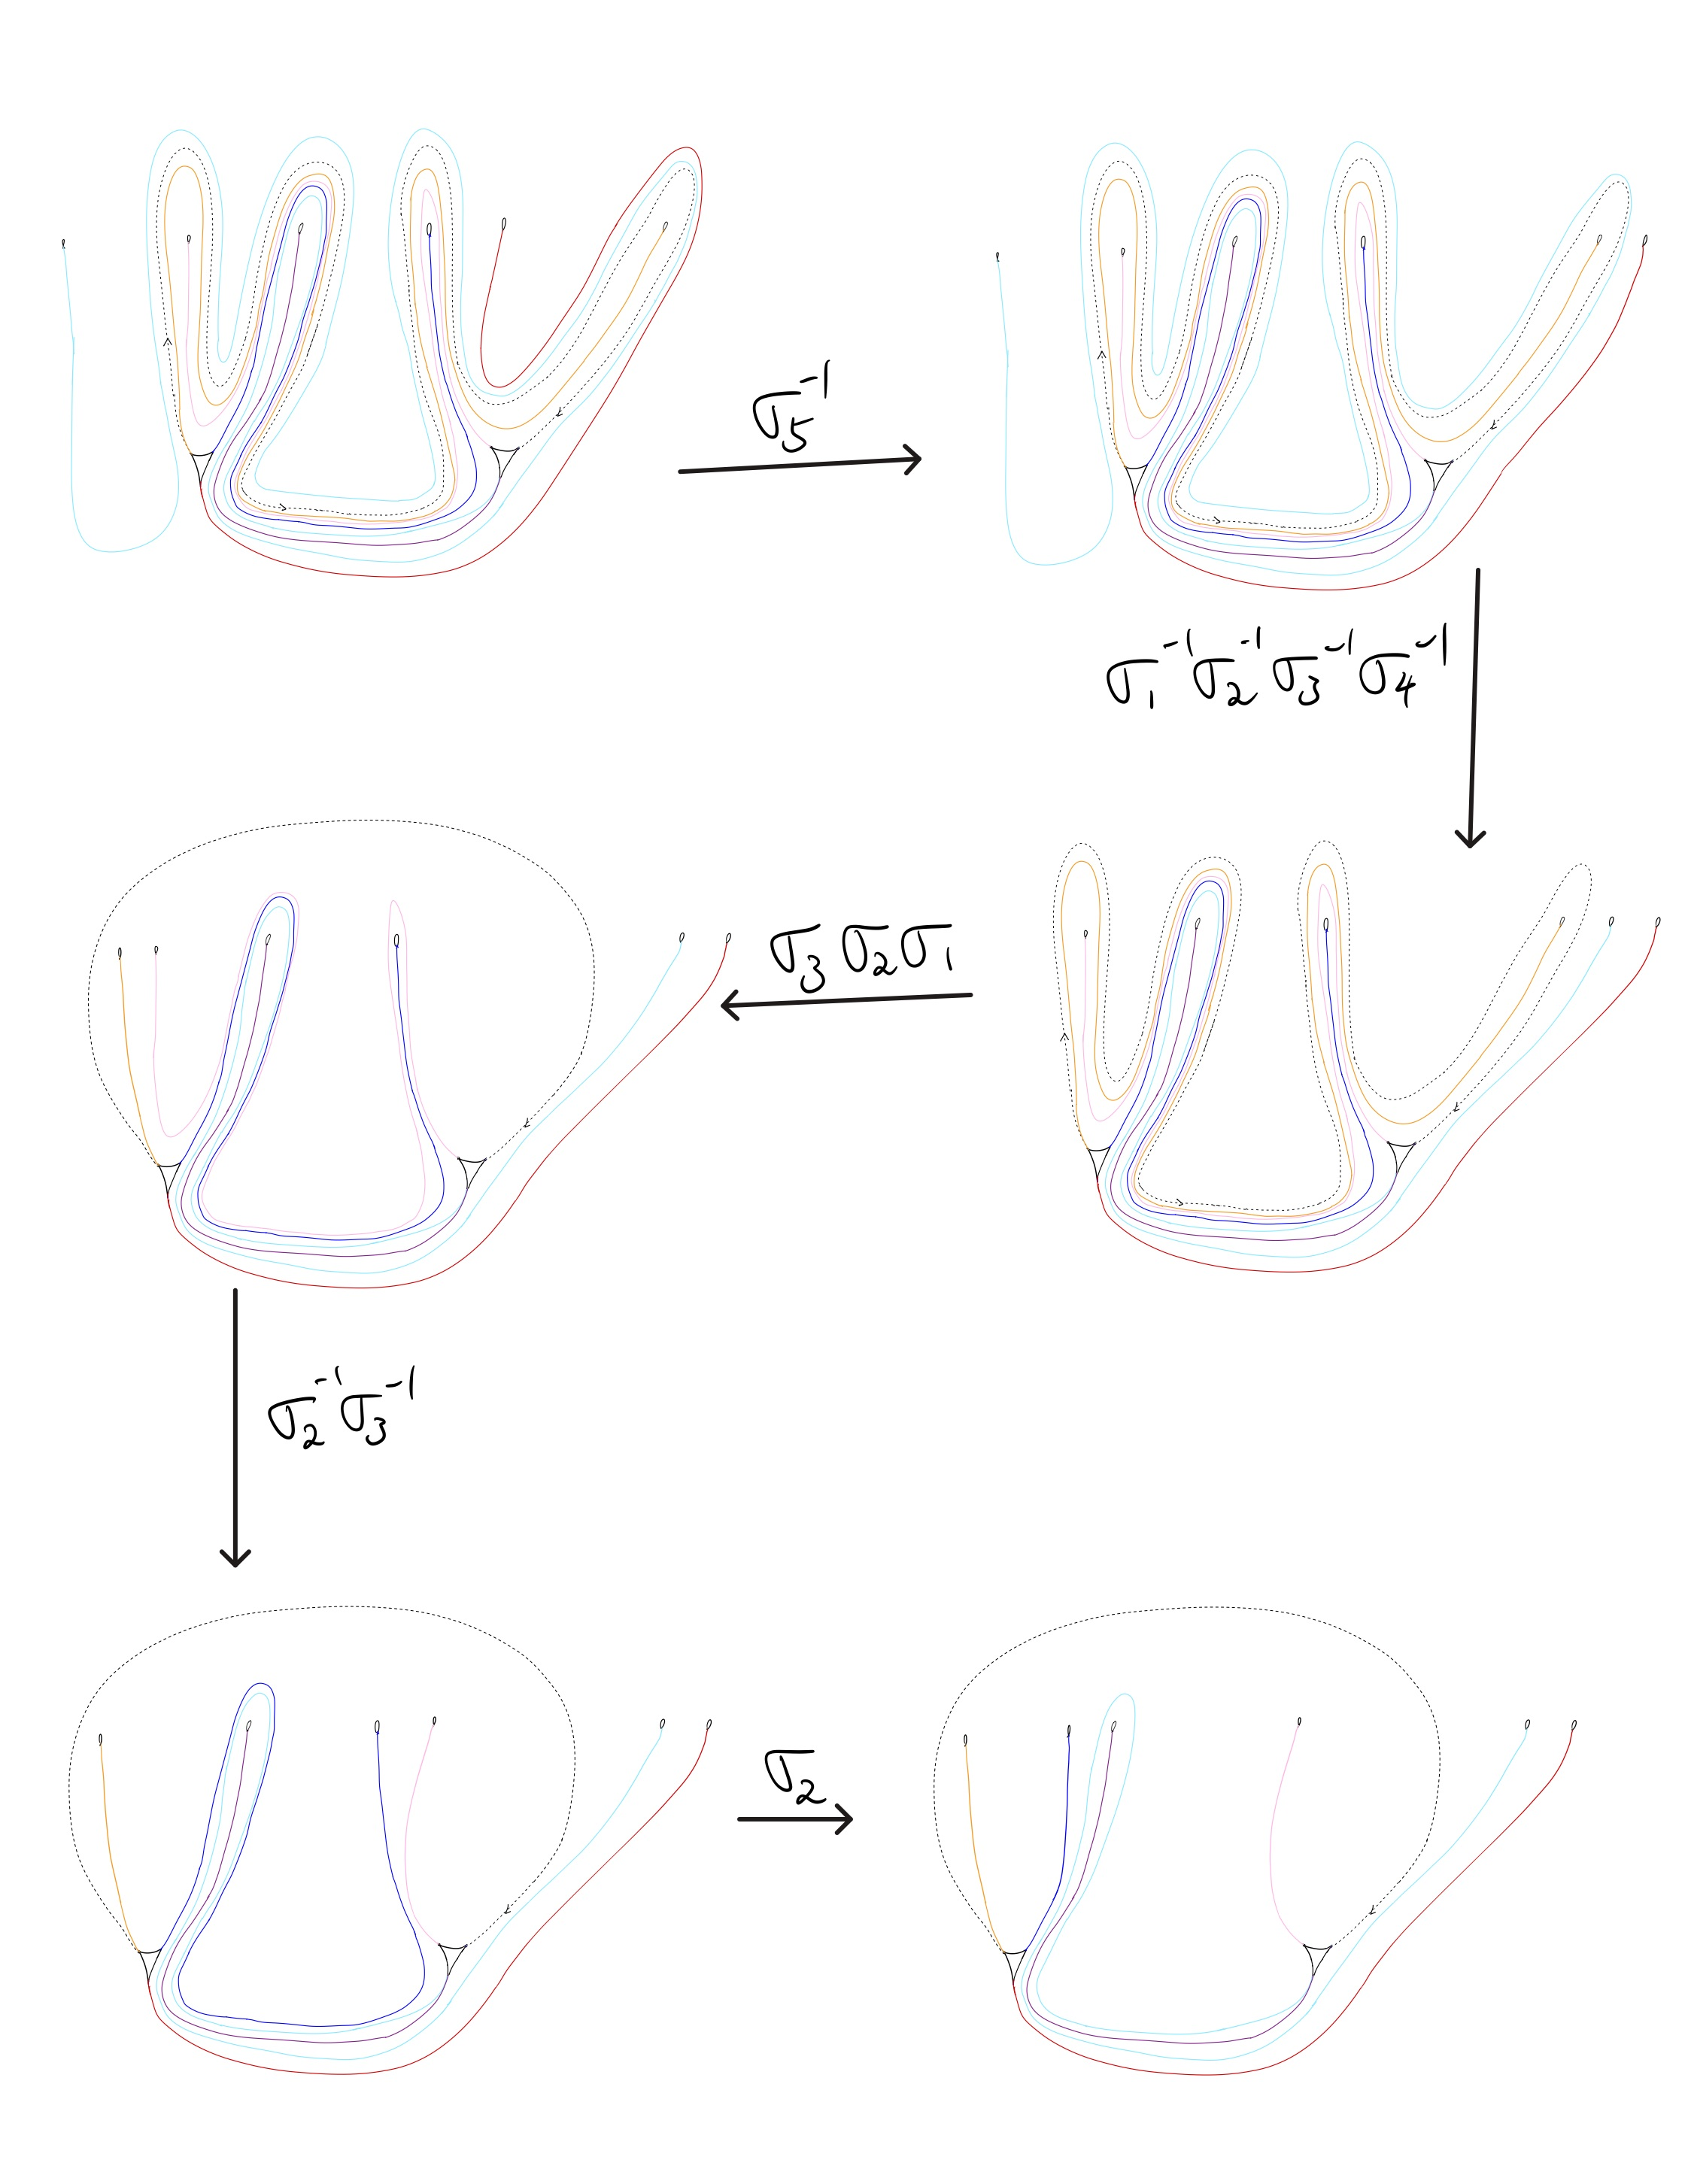
\includegraphics[width=\linewidth, height=0.45\textheight, keepaspectratio]{figures_braid/figures_track_8/Track 8 Braid 8 Oread-2.jpg}%
    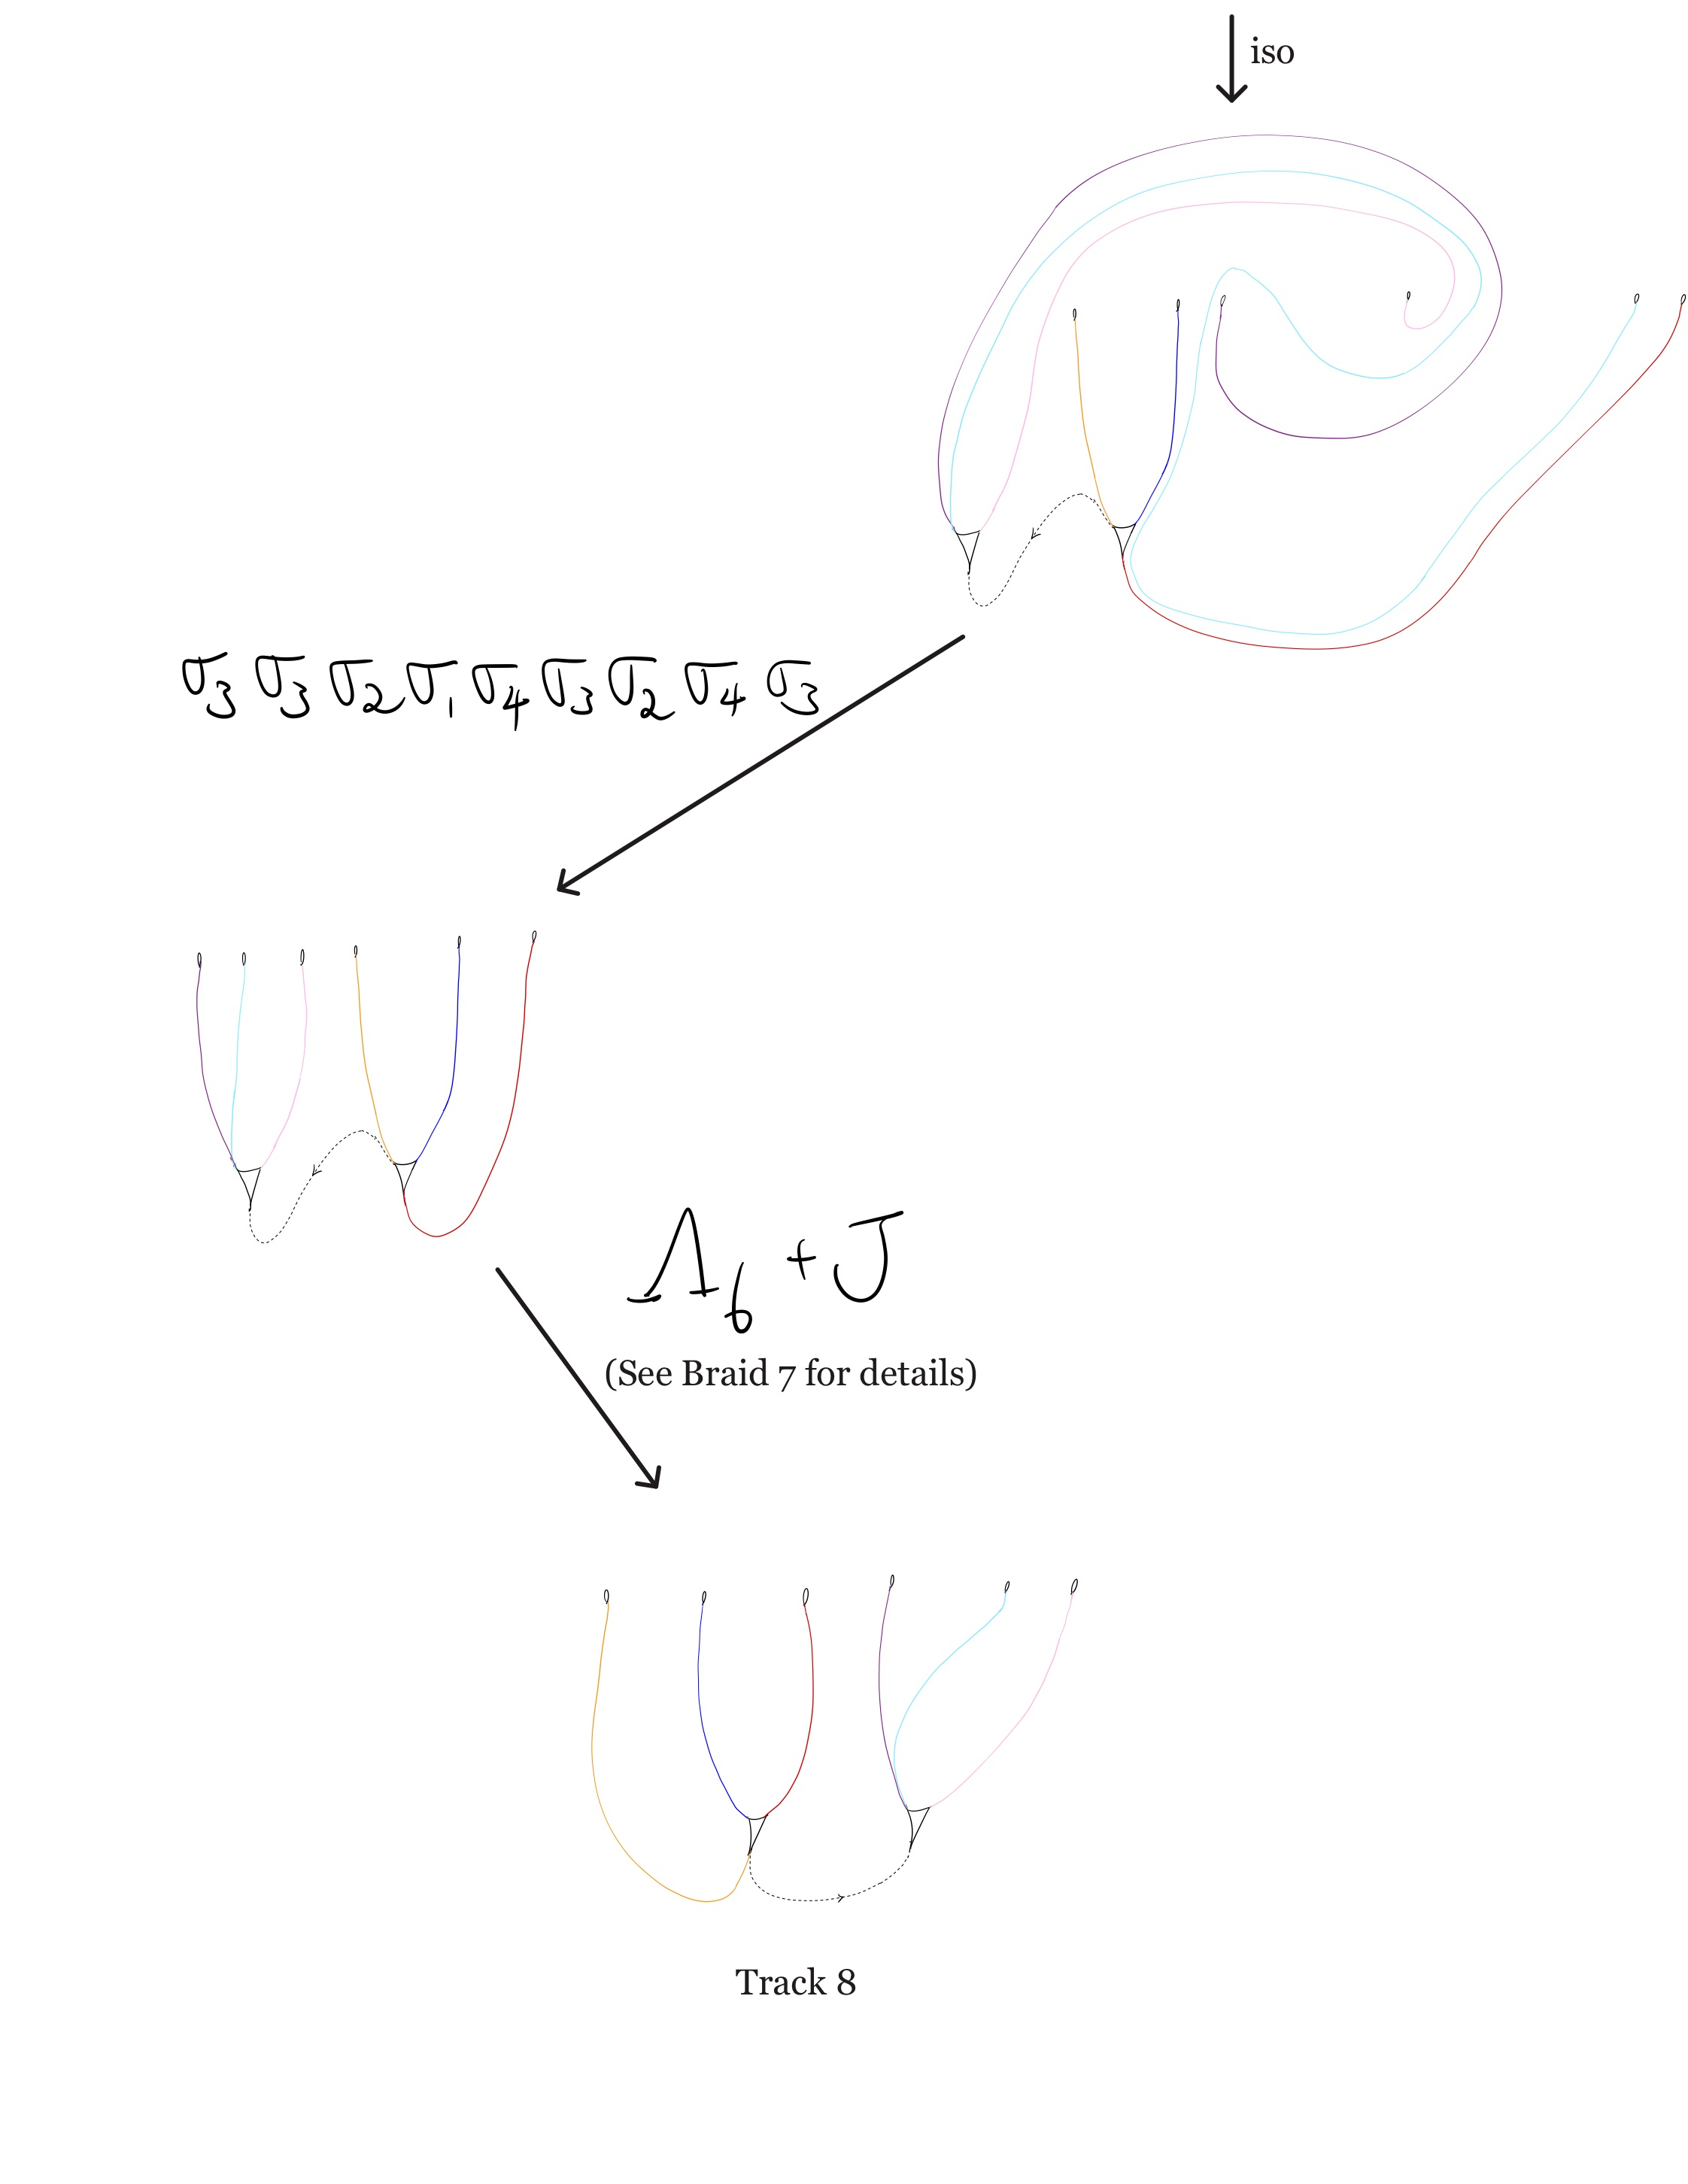
\includegraphics[width=\linewidth, height=0.45\textheight, keepaspectratio]{figures_braid/figures_track_8/Track 8 Braid 8 Oread-3.jpg}
    \caption{This sequence shows the inverse of the braid $b_8^8$ carries Train Track Candidate Family 8.}
    \label{fig:track8_braid_b8_8}
\end{figure*}

\clearpage

\section{Candidate Family 9 (FAT)}\label{sec:track8_fat}
Train Track Map Candidate Family 9 of Track 8 is shown in Figure \ref{fig:track8_braid_b8_9_map}. See \ref{FAT} for details.

\begin{figure*}[ht]
    \centering
    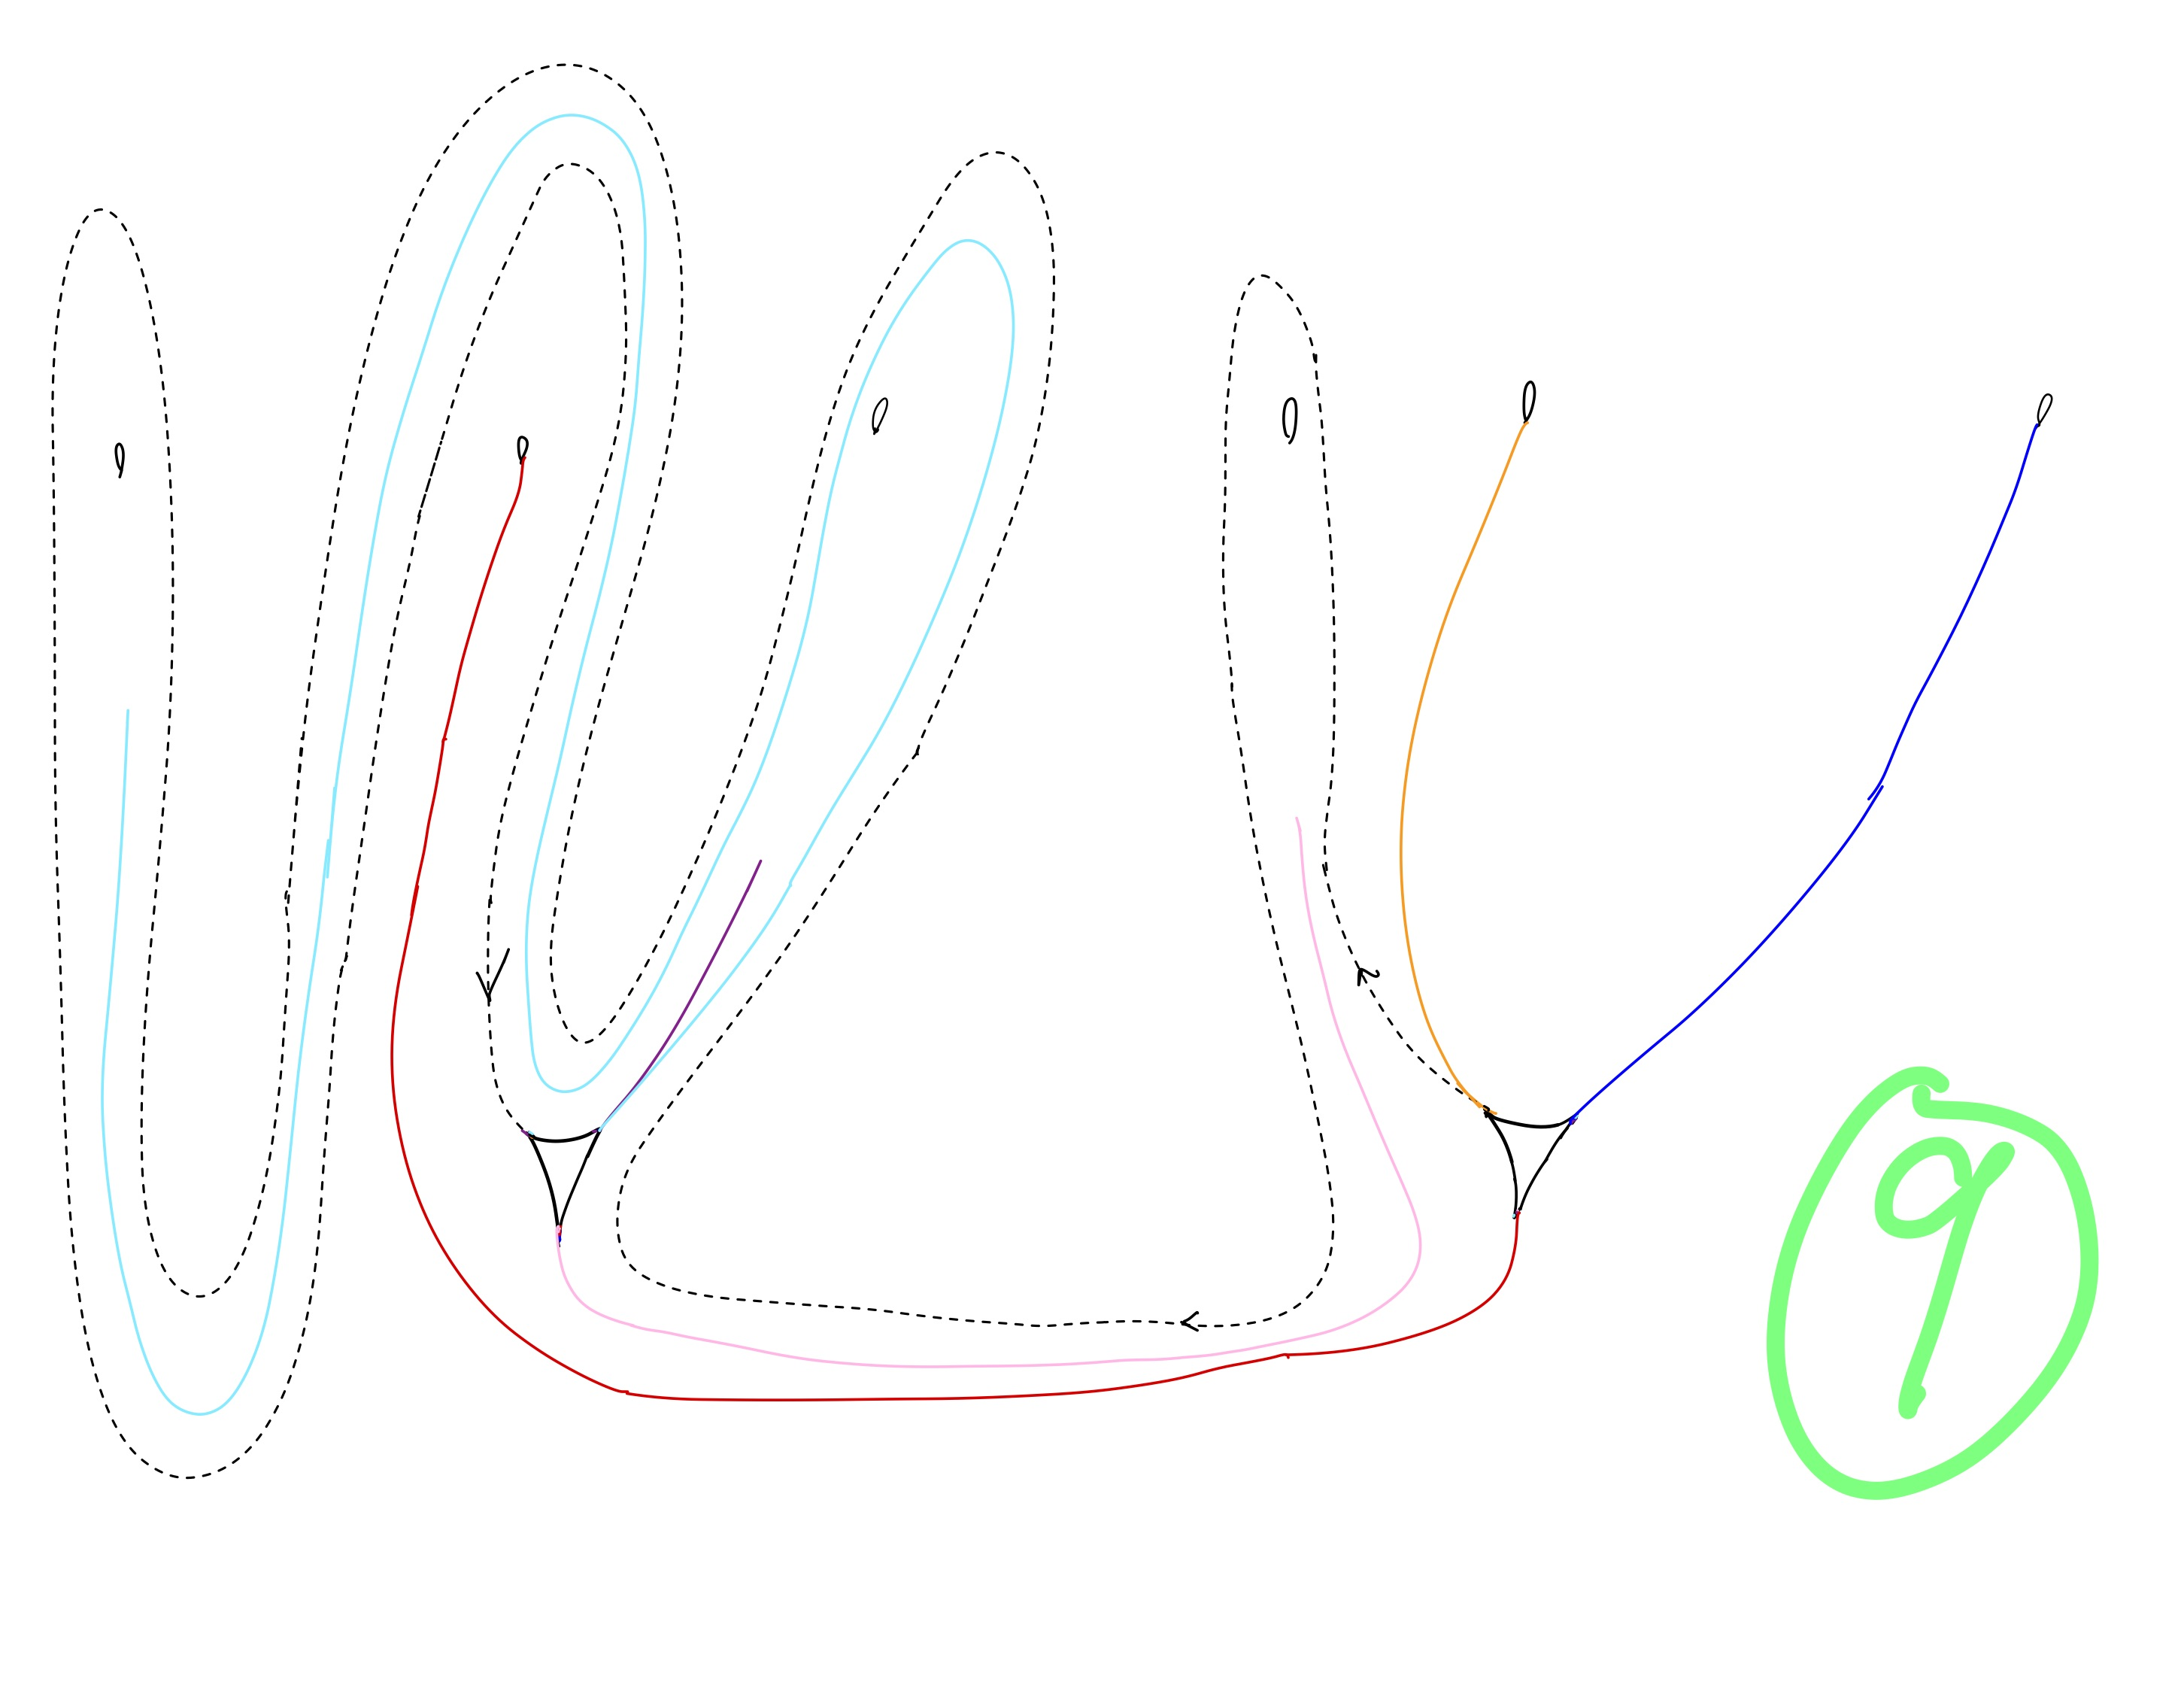
\includegraphics[width=\linewidth, height=0.45\textheight, keepaspectratio]{figures_braid/figures_track_8/Track 8 Braid 9 FAT-1.jpg}
    \caption{Train Track Map Candidate Family 9 (FAT) of Track 8.}
    \label{fig:track8_braid_b8_9_map}
\end{figure*}

The inverse of the following braid carries this family of train track maps:
\[
b_9^8 = \sigma_{1}^{-1} \sigma_{2}^{-k} \sigma_{3}^{-1} \sigma_{2}^{-1} \sigma_{2}^{-1} \sigma_{3}^{-1} \sigma_{2}^{-1} \sigma_{2}^{-1} \sigma_{1} \sigma_{2} \sigma_{3} \sigma_{4} \sigma_{5} \circ \Lambda_6 \circ J
\]
where $k \geq 1$ ($k \in \mathbb{Z}$) is the twisting parameter. This is shown in Figure \ref{fig:track8_braid_b8_9}.

\begin{figure*}[p]
    \centering
    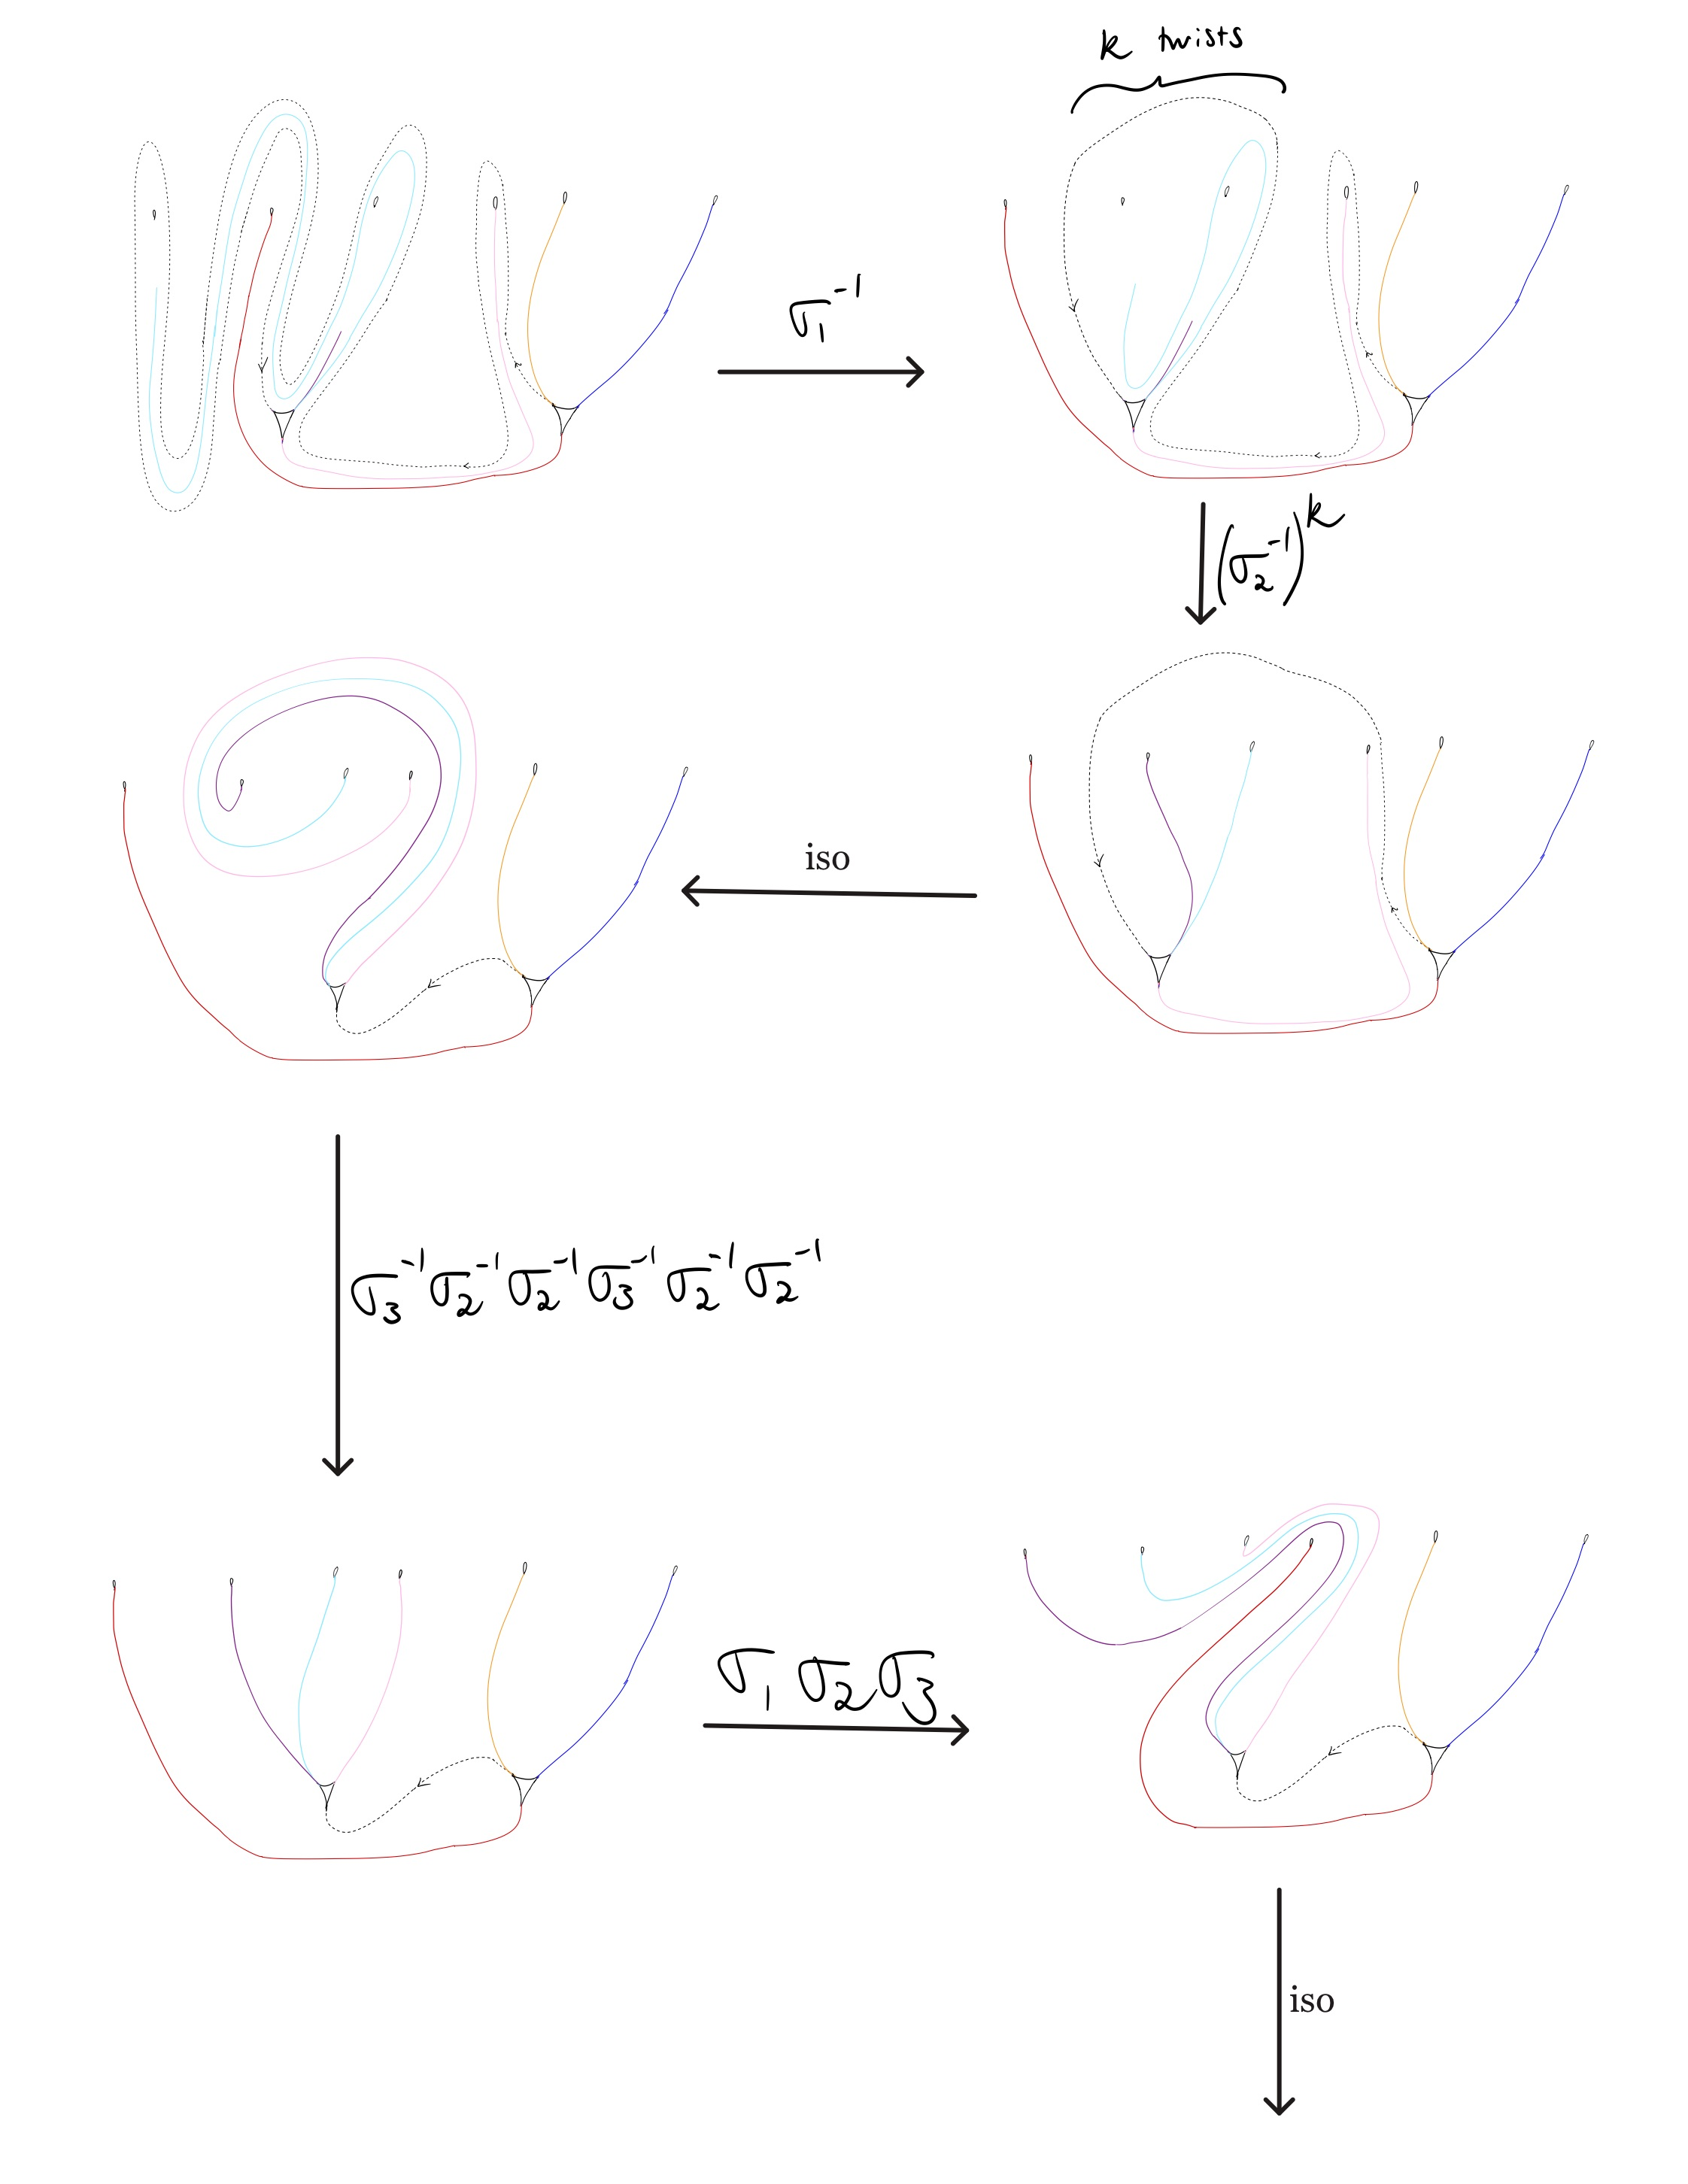
\includegraphics[width=\linewidth, height=0.45\textheight, keepaspectratio]{figures_braid/figures_track_8/Track 8 Braid 9 FAT-2.jpg}%
    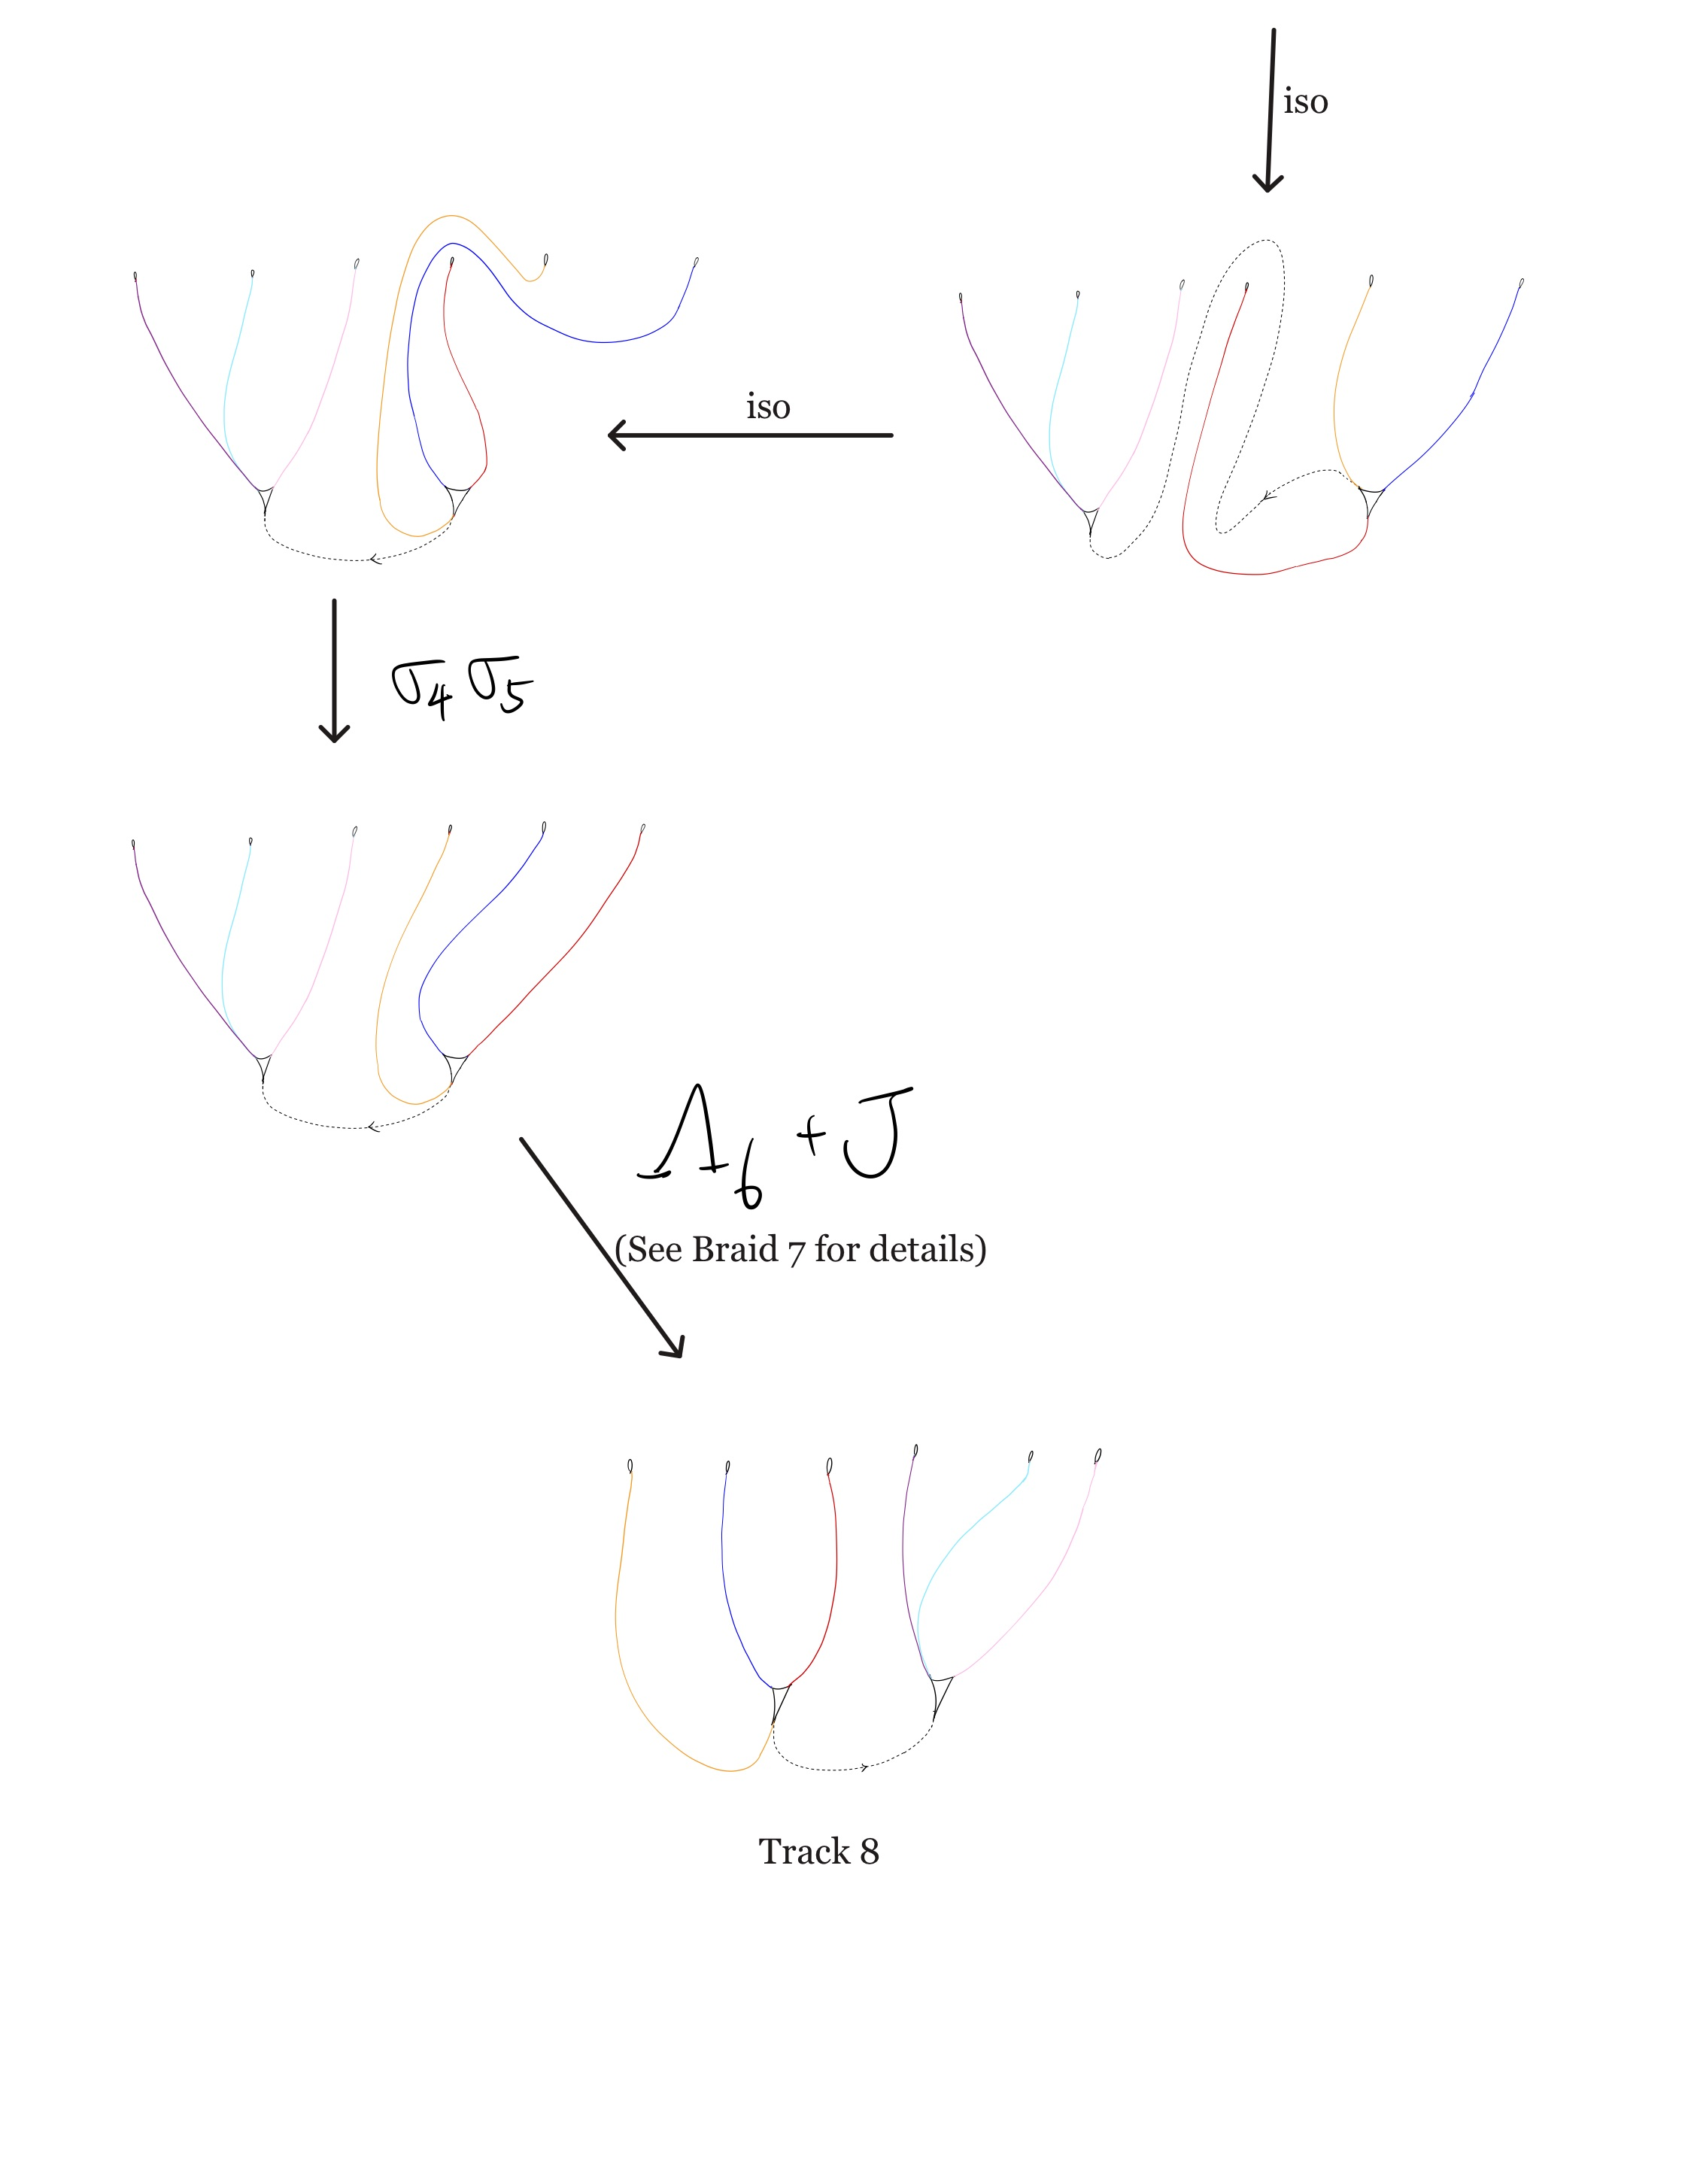
\includegraphics[width=\linewidth, height=0.45\textheight, keepaspectratio]{figures_braid/figures_track_8/Track 8 Braid 9 FAT-3.jpg}
    \caption{This sequence shows the inverse of the braid $b_9^8$ carries Train Track Candidate Family 9.}
    \label{fig:track8_braid_b8_9}
\end{figure*}

\clearpage